% =====================================================================
%  ELL305 Computer Architecture, IIT Delhi -- Final Term Paper
%  Why Two Threads Can See Memory in Different Orders:
%  SC vs TSO from the Ground Up
%
%  One file. The bibliography is embedded below with filecontents*.
%  Build:
%    pdflatex term_paper && bibtex term_paper && makeglossaries term_paper
%    && makeindex term_paper && pdflatex term_paper && pdflatex term_paper
% =====================================================================
\begin{filecontents*}{\jobname.bib}
@book{sarangiBasic,
  author    = {Smruti R. Sarangi},
  title     = {Basic Computer Architecture},
  publisher = {White Falcon Publishing},
  address   = {Chandigarh, India},
  edition   = {version 3.09},
  year      = {2025},
  note      = {\url{https://srsarangi.github.io/archbook/archbook.pdf}}
}
@book{sarangiNextGen,
  author    = {Smruti R. Sarangi},
  title     = {Next-Gen Computer Architecture: Till the End of Silicon},
  publisher = {White Falcon Publishing},
  address   = {Chandigarh, India},
  year      = {2023},
  note      = {\url{https://www.cse.iitd.ac.in/~srsarangi/advbook/nextgen-comp-arch.pdf}}
}
@article{lamport1979,
  author  = {Leslie Lamport},
  title   = {How to Make a Multiprocessor Computer That Correctly Executes Multiprocess Programs},
  journal = {IEEE Transactions on Computers},
  volume  = {C-28},
  number  = {9},
  pages   = {690--691},
  year    = {1979}
}
@inproceedings{owens2009,
  author    = {Scott Owens and Susmit Sarkar and Peter Sewell},
  title     = {A Better x86 Memory Model: x86-{TSO}},
  booktitle = {Theorem Proving in Higher Order Logics (TPHOLs)},
  series    = {Lecture Notes in Computer Science},
  volume    = {5674},
  pages     = {391--407},
  publisher = {Springer},
  year      = {2009}
}
@article{alglave2014,
  author  = {Jade Alglave and Luc Maranget and Michael Tautschnig},
  title   = {Herding Cats: Modelling, Simulation, Testing, and Data Mining for Weak Memory},
  journal = {ACM Transactions on Programming Languages and Systems},
  volume  = {36},
  number  = {2},
  pages   = {7:1--7:74},
  year    = {2014}
}
\end{filecontents*}

\documentclass[12pt,a4paper,twoside,openany]{report}

\usepackage[a4paper,margin=1in]{geometry}
\usepackage[T1]{fontenc}
\usepackage[utf8]{inputenc}
\usepackage{mathpazo}
\renewcommand{\ttdefault}{lmtt}
\renewcommand{\sfdefault}{lmss}
\usepackage{amsmath,amssymb}
\usepackage{setspace}\singlespacing
\usepackage{microtype}
\usepackage{pgfgantt}
\usepackage{xcolor}
\usepackage{graphicx}
\usepackage{float}
\usepackage{booktabs,array,tabularx,longtable,multirow}
\usepackage{enumitem}
\setlist{itemsep=2pt,topsep=4pt}
\usepackage{caption}
\captionsetup{font=small,labelfont=bf,margin=0.5cm}
\usepackage{tikz}
\usetikzlibrary{arrows.meta,positioning,shapes.geometric,shapes.misc,calc,fit,
  backgrounds,decorations.pathreplacing,matrix}
\usepackage{pgfplots}
\pgfplotsset{compat=1.18}
\usepackage{listings}
\usepackage[most]{tcolorbox}
\usepackage[super,sort&compress]{natbib}
\usepackage{imakeidx}
\makeindex[intoc]
\usepackage[hidelinks]{hyperref}
\usepackage[nonumberlist,toc]{glossaries}
\makeglossaries
\usepackage[nameinlink,capitalise]{cleveref}
\crefname{chapter}{Chapter}{Chapters}
\crefname{appendix}{Appendix}{Appendices}

\setlength{\parskip}{3pt}
\renewcommand{\arraystretch}{1.15}

% ---------- colours ---------------------------------------------------
\definecolor{vsbg}{HTML}{1E1E1E}
\definecolor{vsfg}{HTML}{D4D4D4}
\definecolor{vskw}{HTML}{569CD6}
\definecolor{vsctl}{HTML}{C586C0}
\definecolor{vsstr}{HTML}{CE9178}
\definecolor{vscom}{HTML}{6A9955}
\definecolor{vsnum}{HTML}{B5CEA8}
\definecolor{vsln}{HTML}{858585}
\definecolor{vsfn}{HTML}{DCDCAA}
\definecolor{boxblue}{HTML}{E8EEFB}
\definecolor{boxgreen}{HTML}{E6F4EA}
\definecolor{boxorange}{HTML}{FDF0E1}
\definecolor{boxpurple}{HTML}{EFE7F6}
\definecolor{boxgrey}{HTML}{F1F1F1}
\definecolor{edgepo}{HTML}{1F3A93}
\definecolor{edgefr}{HTML}{B03A2E}
\definecolor{edgerf}{HTML}{1E8449}
\definecolor{edgefence}{HTML}{7D3C98}
\definecolor{edgedrop}{HTML}{D68910}
\definecolor{edgeco}{HTML}{9A7D0A}
\definecolor{nodec}{HTML}{8E2455}

% ---------- VS Code style listings ------------------------------------
\lstdefinestyle{vscode}{
  backgroundcolor=\color{vsbg}, basicstyle=\ttfamily\footnotesize\color{vsfg},
  keywordstyle=\color{vskw}, keywordstyle=[2]\color{vsctl},
  commentstyle=\color{vscom}\itshape, stringstyle=\color{vsstr},
  numberstyle=\tiny\color{vsln}, numbers=left, numbersep=6pt,
  xleftmargin=1.6em, framexleftmargin=1.6em, frame=single, rulecolor=\color{vsbg},
  breaklines=true, breakatwhitespace=true, showstringspaces=false,
  tabsize=4, columns=fullflexible, keepspaces=true, upquote=true,
  aboveskip=8pt, belowskip=8pt, literate={~}{{\textasciitilde}}1}
\lstdefinelanguage{Pseudo}{
  morekeywords={for,each,in,if,then,else,return,and,or,not,while,do,end},
  morekeywords=[2]{allowed,edges,model},
  morecomment=[l]{\#}, sensitive=true}
\lstdefinelanguage{asmx}{
  morekeywords={mov,movl,mfence,xchg,ret,endbr64,lock,orq,nop,nopl},
  morecomment=[l]{\#}, sensitive=true}
\lstset{style=vscode}
\lstdefinestyle{vspython}{style=vscode,language=Python,
  morekeywords=[2]{for,in,if,else,elif,return,while,import,from,def,class,with,not,and,or,is,None,True,False,yield}}
\lstdefinestyle{vsc}{style=vscode,language=C,
  morekeywords={_Atomic,atomic_store_explicit,atomic_load_explicit,__asm__,__volatile__,__attribute__}}

% ---------- result boxes -----------------------------------------------
\newtcolorbox{resultbox}[1]{colback=boxgreen,colframe=edgerf!80!black,
  fonttitle=\bfseries\small,title={#1},boxrule=0.6pt,arc=2pt,
  left=6pt,right=6pt,top=3pt,bottom=3pt}
\newtcolorbox{forbidbox}[1]{colback=boxorange,colframe=edgefr!85!black,
  fonttitle=\bfseries\small,title={#1},boxrule=0.6pt,arc=2pt,
  left=6pt,right=6pt,top=3pt,bottom=3pt}
\newtcolorbox{notebox}{colback=boxblue,colframe=edgepo!70!black,boxrule=0.5pt,
  arc=2pt,left=6pt,right=6pt,top=3pt,bottom=3pt}

% ---------- TikZ styles --------------------------------------------------
\tikzset{
  ev/.style={draw, rounded corners=2pt, fill=boxblue, minimum width=2.4cm,
    minimum height=0.85cm, font=\ttfamily\small},
  blk/.style={draw, rounded corners=3pt, fill=boxblue, align=center,
    font=\small, minimum height=0.9cm, inner sep=4pt},
  po/.style={-{Stealth[length=3mm]}, very thick, edgepo},
  fr/.style={-{Stealth[length=3mm]}, very thick, edgefr},
  rf/.style={-{Stealth[length=3mm]}, very thick, edgerf},
  co/.style={-{Stealth[length=3mm]}, very thick, edgeco},
  gn/.style={circle, draw=black, text=black, very thick, fill=white, minimum size=0.85cm, inner sep=0pt, font=\normalsize\bfseries},
  el/.style={font=\scriptsize\bfseries, inner sep=1.5pt, midway, auto},
  fenceedge/.style={-{Stealth[length=3mm]}, very thick, edgefence},
  dropped/.style={-{Stealth[length=2.5mm]}, thick, edgedrop},
  lab/.style={font=\scriptsize, fill=white, inner sep=1.5pt},
  arr/.style={-{Stealth[length=2.5mm]}, thick},
}

% ---------- macros ---------------------------------------------------------
\newcommand{\rel}[1]{\textsf{#1}}            % relation names: po, rf ...
\newcommand{\po}{\rel{po}}
\newcommand{\rf}{\rel{rf}}
\newcommand{\co}{\rel{co}}
\newcommand{\fr}{\rel{fr}}
\newcommand{\ppo}{\rel{ppo}}
\newcommand{\rfe}{\rel{rfe}}
\newcommand{\poloc}{\rel{po-loc}}
\newcommand{\code}[1]{\texttt{#1}}
\newcommand{\outc}[2]{$(#1,#2)$}
\newcommand{\repourl}{\url{https://github.com/y4shv/ELL-Term-paper}}
\newcommand{\WR}{W$\to$R}
\newcommand{\WW}{W$\to$W}
\newcommand{\RR}{R$\to$R}
\newcommand{\RW}{R$\to$W}

% ---------- glossary ---------------------------------------------------------
\newglossaryentry{litmus}{text={litmus test},name={litmus test},description={A tiny program, usually of two threads, written to check one ordering rule. It always asks whether one particular final outcome is possible}}
\newglossaryentry{po}{text={program order},name={program order (po)},description={The order of instructions inside one thread, as written in the program. It never links two different threads}}
\newglossaryentry{rf}{text={reads-from},name={reads-from (rf)},description={An arrow from a write to the read that got its value from that write}}
\newglossaryentry{co}{text={coherence order},name={coherence order (co)},description={For one address, the order in which all its writes take effect. The initial write comes first}}
\newglossaryentry{fr}{text={from-read},name={from-read (fr)},description={An arrow from a read to every write that is later than the write it read from. The read saw an older value, so it must come before the newer write}}
\newglossaryentry{ppo}{text={preserved program order},name={preserved program order (ppo)},description={The part of program order that a memory model promises to keep}}
\newglossaryentry{sb}{name={store buffer},description={A small first-in, first-out queue between a core and its cache that holds writes, so that the core does not wait for them}}
\newglossaryentry{fwd}{name={store-to-load forwarding},description={A read that finds a matching write in its own core's store buffer takes the value from there instead of from the cache}}
\newglossaryentry{coh}{name={cache coherence},description={The guarantee that all cores agree on one order of the writes to each single address}}
\newglossaryentry{scl}{name={SC per location},description={Accesses to one single address always behave as if the machine were sequentially consistent. It holds in every model in this paper}}
\newglossaryentry{fence}{name={fence},description={An instruction that makes the memory operations before it come before the memory operations after it}}
\newglossaryentry{squash}{name={squash},description={Throwing away work that a core did on a guess, and doing it again}}
\newglossaryentry{drfsc}{name={DRF-SC},description={The promise that a program free of data races behaves as if the machine were sequentially consistent}}
\newglossaryentry{pso}{name={PSO},description={Partial Store Order. TSO plus one more freedom: writes to different addresses may become visible in a different order}}
\newglossaryentry{tso}{name={TSO},description={Total Store Order. Like SC, except that a write may become visible to other cores after a later read of the same thread}}
\newglossaryentry{sc}{name={SC},description={Sequential Consistency. Everything behaves as if all instructions of all threads ran one at a time in a single order that keeps each thread's program order}}
\newglossaryentry{rot}{name={rule of three},description={If an event is seen zero times in N independent tries, its true probability is below about 3/N with 95 per cent confidence}}

\definecolor{cychl}{HTML}{F4D03F}
\def\cycword{cyc}
% ---- litmus graph panels (circular nodes, built step by step) ----
% \sbpanel{prefix}{stage}{po kept? 1/0}{note under the panel}
\newcommand{\sbpanel}[4]{%
  \node[gn] (#1a) at (0,2) {a};
  \node[gn] (#1b) at (0,0) {b};
  \node[gn] (#1c) at (3.8,2) {c};
  \node[gn] (#1d) at (3.8,0) {d};
  \node[gn] (#1e) at (1.9,3.3) {e};
  \node[gn] (#1f) at (1.9,-1.3) {f};
  \def\tmpnote{#4}
  \ifnum#2=4 \ifx\tmpnote\cycword
    \draw[cychl, line width=9pt, opacity=0.7, line cap=round] (#1a) -- (#1b);
    \draw[cychl, line width=9pt, opacity=0.7, line cap=round] (#1c) -- (#1d);
    \draw[cychl, line width=9pt, opacity=0.7, line cap=round] (#1b) to[bend left=12] (#1c);
    \draw[cychl, line width=9pt, opacity=0.7, line cap=round] (#1d) to[bend left=12] (#1a);
  \fi\fi
  \ifnum#3=1
    \draw[po] (#1a) -- node[el, text=edgepo] {po} (#1b);
    \draw[po] (#1c) -- node[el, text=edgepo] {po} (#1d);
  \fi
  \ifnum#3=2
    \draw[fenceedge] (#1a) -- node[el, text=edgefence] {mfence} (#1b);
    \draw[fenceedge] (#1c) -- node[el, text=edgefence] {mfence} (#1d);
  \fi
  \ifnum#3=0
    \ifnum#2=1
      \draw[dropped] (#1a) -- node[el, text=edgedrop] {dropped} (#1b);
      \draw[dropped] (#1c) -- node[el, text=edgedrop] {dropped} (#1d);
    \fi
  \fi
  \ifnum#2>1
    \draw[rf] (#1f) -- node[el, text=edgerf, pos=0.35] {rf} (#1b);
    \draw[rf] (#1e) -- node[el, text=edgerf, pos=0.3] {rf} (#1d);
  \fi
  \ifnum#2>2
    \draw[co] (#1e) -- node[el, text=edgeco] {co} (#1a);
    \draw[co] (#1f) -- node[el, text=edgeco] {co} (#1c);
  \fi
  \ifnum#2>3
    \draw[fr] (#1b) to[bend left=12] node[el, text=edgefr, pos=0.3] {fr} (#1c);
    \draw[fr] (#1d) to[bend left=12] node[el, text=edgefr, pos=0.3] {fr} (#1a);
  \fi
  \ifnum#2=4 \ifx\tmpnote\cycword\else \node[font=\scriptsize, text=edgefr, align=center] at (1.9,-2.3) {#4}; \fi\fi
}
% \mppanel{prefix}{stage}{first po (W->W) kept? 1/0}{note}
\newcommand{\mppanel}[4]{%
  \node[gn] (#1a) at (0,2) {a};
  \node[gn] (#1b) at (0,0) {b};
  \node[gn] (#1c) at (3.8,2) {c};
  \node[gn] (#1d) at (3.8,0) {d};
  \node[gn] (#1e) at (1.9,3.3) {e};
  \node[gn] (#1f) at (0,-1.3) {f};
  \def\tmpnote{#4}
  \ifnum#2=4 \ifx\tmpnote\cycword
    \draw[cychl, line width=9pt, opacity=0.7, line cap=round] (#1a) -- (#1b);
    \draw[cychl, line width=9pt, opacity=0.7, line cap=round] (#1b) -- (#1c);
    \draw[cychl, line width=9pt, opacity=0.7, line cap=round] (#1c) -- (#1d);
    \draw[cychl, line width=9pt, opacity=0.7, line cap=round] (#1d) to[bend left=12] (#1a);
  \fi\fi
  \ifnum#3=1
    \draw[po] (#1a) -- node[el, text=edgepo] {po} (#1b);
  \fi
  \ifnum#3=2
    \draw[fenceedge] (#1a) -- node[el, text=edgefence] {stbar} (#1b);
  \fi
  \ifnum#3=0
    \ifnum#2=1
      \draw[dropped] (#1a) -- node[el, text=edgedrop] {dropped} (#1b);
    \fi
  \fi
  \draw[po] (#1c) -- node[el, text=edgepo] {po} (#1d);
  \ifnum#2>1
    \draw[rf] (#1b) -- node[el, text=edgerf, pos=0.3] {rf} (#1c);
    \draw[rf] (#1e) -- node[el, text=edgerf, pos=0.3] {rf} (#1d);
  \fi
  \ifnum#2>2
    \draw[co] (#1e) -- node[el, text=edgeco] {co} (#1a);
    \draw[co] (#1f) -- node[el, text=edgeco] {co} (#1b);
  \fi
  \ifnum#2>3
    \draw[fr] (#1d) to[bend left=12] node[el, text=edgefr, pos=0.3] {fr} (#1a);
  \fi
  \ifnum#2=4 \ifx\tmpnote\cycword\else \node[font=\scriptsize, text=edgefr, align=center] at (1.9,-2.3) {#4}; \fi\fi
}
% four panels in a 2x2 block: \fourpanels{\sbpanel or \mppanel}{kept}{note}
\newcommand{\fourpanels}[3]{%
\begin{tikzpicture}[scale=0.9, transform shape]
  \begin{scope}[shift={(0,0)}]
    \node[font=\small\bfseries] at (1.9,4.2) {1. program order};
    #1{p}{1}{#2}{#3}
  \end{scope}
  \begin{scope}[shift={(7.0,0)}]
    \node[font=\small\bfseries] at (1.9,4.2) {2. add reads-from};
    #1{q}{2}{#2}{#3}
  \end{scope}
  \begin{scope}[shift={(0,-6.8)}]
    \node[font=\small\bfseries] at (1.9,4.2) {3. add coherence order};
    #1{r}{3}{#2}{#3}
  \end{scope}
  \begin{scope}[shift={(7.0,-6.8)}]
    \node[font=\small\bfseries] at (1.9,4.2) {4. add from-read};
    #1{s}{4}{#2}{#3}
  \end{scope}
\end{tikzpicture}}

\begin{document}
\pagenumbering{arabic}

% ---------------------------------------------------------------- title
\begin{titlepage}
\centering
\vspace*{1.2cm}
{\LARGE\bfseries Memory Consistency Models\par}
\vspace{0.5cm}
{\Large SC, TSO and PSO\par}
\vspace{0.8cm}
{\large ELL305 Computer Architecture\\ Final Term Paper\par}
\vspace{1.6cm}
{\large November 2026\par}
\vspace{1.8cm}
\begin{tabular}{ll}
\toprule
\textbf{Name} & \textbf{Entry number}\\
\midrule
Dhruv Mittal & 2024MT60812\\
Arnav Singh & 2024MT60027\\
Yash Vashisht & 2024MT60062\\
Aditya & 2024MT10096\\
Kashav Kumar & 2024MT10040\\
Parth Aggarwal & 2024EE10893\\
\bottomrule
\end{tabular}
\vfill
{Advisor: Prof. Subrat Kar\\
Department of Electrical Engineering, Indian Institute of Technology Delhi\par}
\vspace{0.6cm}
\centering 1
\end{titlepage}
\setcounter{page}{2}

% ---------------------------------------------------------------- copyright
\chapter*{Copyright}
\addcontentsline{toc}{chapter}{Copyright}
Copyright \textcopyright\ 2026 by the authors listed above. All rights reserved.

This report was prepared as coursework for ELL305 Computer Architecture at the Indian Institute of Technology Delhi. All intellectual property rights in the original material contained in this report vest in the Indian Institute of Technology Delhi. Material quoted, reproduced, adapted, or cited from other sources, including textbooks, papers and software documentation, remains the intellectual property of its respective authors and publishers, and is identified as such at its point of use; its inclusion here is for academic, non-commercial purposes only.

% ---------------------------------------------------------------- acknowledgement
\chapter*{Acknowledgement}
\addcontentsline{toc}{chapter}{Acknowledgement}
We thank Prof. Sumantra Dutta Roy, who taught ELL305, and Prof. Subrat Kar, our term paper advisor, for his guidance on the scope of this project. We also thank Prof. Smruti R. Sarangi, whose two books gave us both the starting point and most of the building blocks of this paper.

We also acknowledge the Department of Electrical Engineering and the Indian Institute of Technology Delhi for the use of their resources in the preparation of this report.


% ---------------------------------------------------------------- abbreviations
\chapter*{Abbreviations}
\addcontentsline{toc}{chapter}{Abbreviations}
\begin{center}
\small
\begin{tabular}{@{}ll@{\hspace{1.2cm}}ll@{}}
SC & Sequential Consistency & SB & Store Buffering (litmus test)\\
TSO & Total Store Order & MP & Message Passing (litmus test)\\
PSO & Partial Store Order & FIFO & First In, First Out\\
CPI & Cycles Per Instruction & DRF & Data-Race-Free\\
MESI & Modified, Exclusive, Shared, Invalid & L1 & first-level cache\\
po & program order & rf & reads-from\\
co & coherence order & fr & from-read\\
ppo & preserved program order & rfe & reads-from, external\\
\end{tabular}
\end{center}

\tableofcontents
\listoffigures
\listoftables

% ---------------------------------------------------------------- map
\chapter*{Map of the Paper}
\addcontentsline{toc}{chapter}{Map of the Paper}
\begin{center}
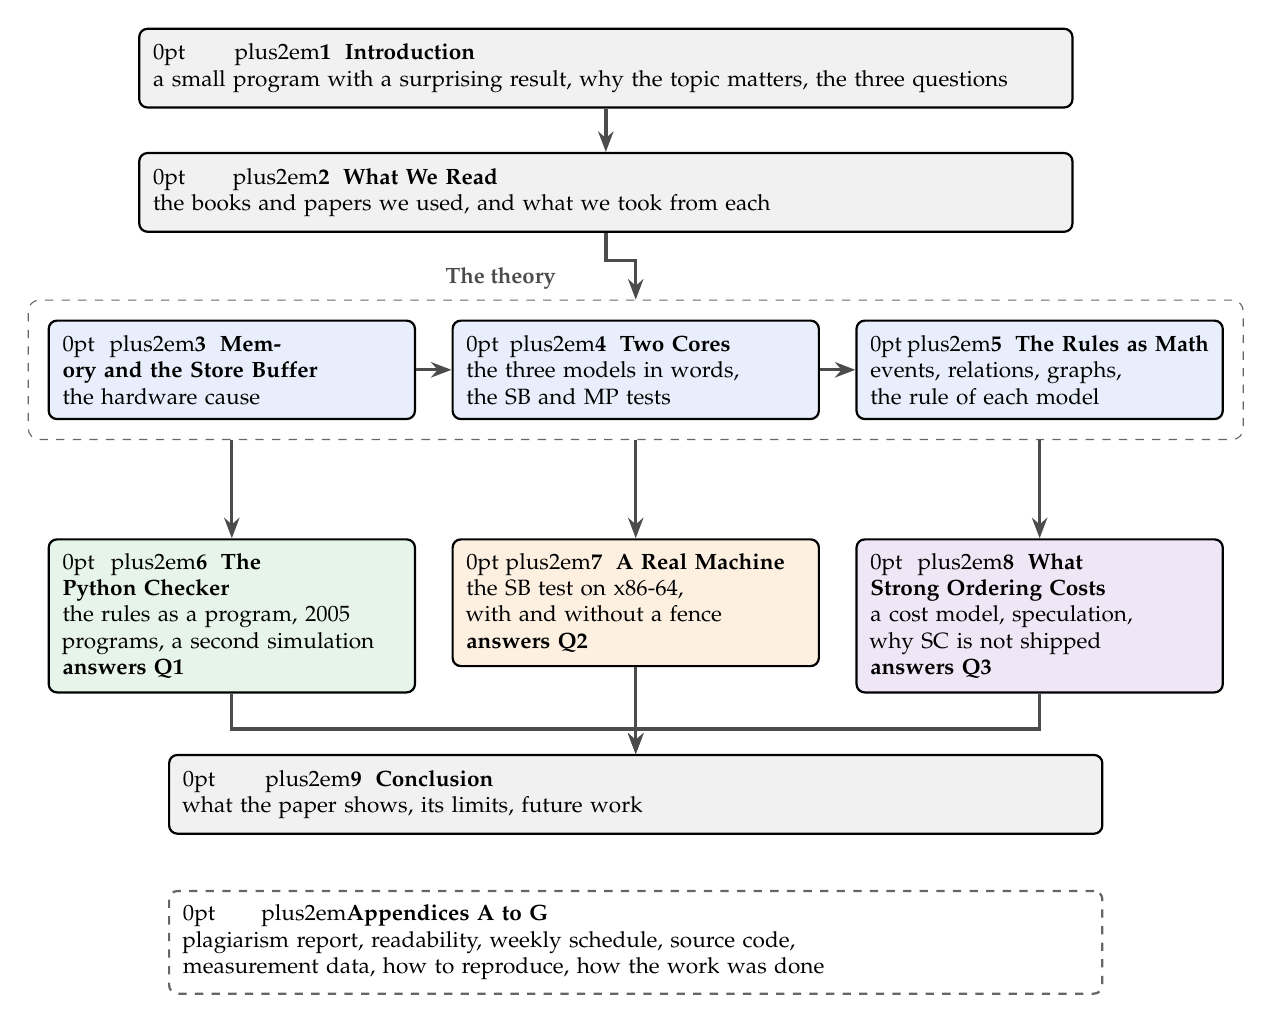
\begin{tikzpicture}[
  bx/.style={draw, rounded corners=3pt, thick, align=center, font=\footnotesize\hyphenpenalty=10000 , inner sep=5pt, text width=4.3cm, minimum height=1.25cm},
  wide/.style={bx, text width=11.5cm, minimum height=1.0cm},
  ar/.style={-{Stealth[length=2.6mm]}, very thick, draw=black!70}]
\node[wide, fill=boxgrey] (c1) {\textbf{1\; Introduction}\\ a small program with a surprising result, why the topic matters, the three questions};
\node[wide, fill=boxgrey, below=0.55cm of c1] (c2) {\textbf{2\; What We Read}\\ the books and papers we used, and what we took from each};
\node[bx, fill=boxblue, below=1.1cm of c2, xshift=-4.75cm] (c3) {\textbf{3\; Memory and the Store Buffer}\\ the hardware cause};
\node[bx, fill=boxblue, right=0.45cm of c3] (c4) {\textbf{4\; Two Cores}\\ the three models in words, the SB and MP tests};
\node[bx, fill=boxblue, right=0.45cm of c4] (c5) {\textbf{5\; The Rules as Math}\\ events, relations, graphs, the rule of each model};
\node[draw=black!60, dashed, rounded corners=4pt, inner sep=7pt, fit=(c3)(c4)(c5), label={[font=\footnotesize\bfseries, text=black!70]above left:The theory}] (theory) {};
\node[bx, fill=boxgreen, below=1.5cm of c3] (c6) {\textbf{6\; The Python Checker}\\ the rules as a program, 2005 programs, a second simulation\\ \textbf{answers Q1}};
\node[bx, fill=boxorange, below=1.5cm of c4] (c7) {\textbf{7\; A Real Machine}\\ the SB test on x86-64, with and without a fence\\ \textbf{answers Q2}};
\node[bx, fill=boxpurple, below=1.5cm of c5] (c8) {\textbf{8\; What Strong Ordering Costs}\\ a cost model, speculation, why SC is not shipped\\ \textbf{answers Q3}};
\node[wide, fill=boxgrey, below=1.1cm of c7] (c9) {\textbf{9\; Conclusion}\\ what the paper shows, its limits, future work};
\node[wide, draw=black!60, dashed, fill=white, below=0.7cm of c9] (app) {\textbf{Appendices A to G}\\ plagiarism report, readability, weekly schedule, source code, measurement data, how to reproduce, how the work was done};
\draw[ar] (c1) -- (c2);
\draw[ar] (c2.south) -- ++(0,-0.35) -| (theory.north);
\draw[ar] (c3) -- (c4);
\draw[ar] (c4) -- (c5);
\draw[ar] (theory.south -| c3) -- (c6);
\draw[ar] (theory.south -| c4) -- (c7);
\draw[ar] (theory.south -| c5) -- (c8);
\draw[ar] (c6.south) -- ++(0,-0.45) -| (c9.north);
\draw[ar] (c7) -- (c9);
\draw[ar] (c8.south) -- ++(0,-0.45) -| (c9.north);
\end{tikzpicture}
\end{center}
\clearpage

% =====================================================================
\chapter{Introduction}
\label{ch:intro}
% =====================================================================

\section{A small program with a surprising result}
\label{sec:intro-sb}

We start with the smallest example we can think of. We take a processor with two cores. Each core runs one thread, so there are two threads in all. Both threads use the same two variables, \code{x} and \code{y}, which sit in the shared memory and start at zero. Each thread has only two instructions. Thread 0 writes 1 to \code{x} and then reads \code{y} into its private register \code{r0}. Thread 1 does the mirror image: it writes 1 to \code{y} and then reads \code{x} into its own register \code{r1}.

\begin{center}
\begin{minipage}{0.38\textwidth}
\centering\textbf{Thread 0 (core 0)}
\begin{lstlisting}[style=vsc,numbers=none]
x = 1;
r0 = y;
\end{lstlisting}
\end{minipage}\hspace{1cm}
\begin{minipage}{0.38\textwidth}
\centering\textbf{Thread 1 (core 1)}
\begin{lstlisting}[style=vsc,numbers=none]
y = 1;
r1 = x;
\end{lstlisting}
\end{minipage}
\end{center}

The question is simple. When both threads have finished, which pairs of values $(\code{r0}, \code{r1})$ can we end up with?

\paragraph{How we normally think.} We read a program one instruction at a time, and we assume that each instruction is finished the moment we get to it. A write to memory is done as soon as it is executed, and the next read sees it. For two threads this means that the four instructions are mixed into one single line, and each thread keeps its own order inside that line. We now test this picture. Suppose \code{r0} ends as 0. Then Thread 0 read \code{y} before Thread 1 wrote 1 to it. Thread 1 reads \code{x} after it has written \code{y}, so its read comes later still. By then Thread 0 has already written \code{x = 1}, because that write came before Thread 0's own read. So Thread 1 sees 1 and \code{r1} is 1. The same argument works the other way round. In short, at least one of the two registers must end up as 1, and the result $\code{r0} = 0,\ \code{r1} = 0$ looks impossible. This way of thinking has a name, \emph{sequential consistency}, or \gls{sc}, and we meet it properly in the next chapters.

\paragraph{What the hardware does.} A real core does not wait for a write to finish. Writing is slow, so each core puts its write into a small waiting queue of its own, called a \emph{\gls{sb}}, and moves on to the next instruction at once. The write is copied from the buffer into the core's cache a little later, and only then can the other core see it. Now run our program again. Core 0 puts \code{x = 1} in its buffer and goes on to read \code{y}. Core 1 has also only put \code{y = 1} in its buffer, so \code{y} is still 0 for everybody else, and core 0 reads 0. Core 1 does the same with \code{x} and reads 0. Both reads slip in front of both writes, and we get $\code{r0} = 0,\ \code{r1} = 0$. The rulebooks that allow this are called Total Store Order (\gls{tso}) and Partial Store Order (\gls{pso}). An ordinary x86-64 processor follows TSO.

\paragraph{Why the result is allowed.} Nothing is broken, in the hardware or in our reasoning. The reasoning above assumed that every write becomes visible to every core immediately, which is the assumption of SC. A machine that follows TSO or PSO makes no such promise, so for that machine the result is allowed. Whether a result is allowed or not depends on the rulebook the machine follows. This rulebook is called a \emph{memory consistency model}\index{memory consistency model}, and this paper is about it. We ask what SC, TSO and PSO allow, we show how to decide this using arrows between the operations, and we check on a real x86-64 machine (\cref{ch:hw}) whether the result really appears.

\section{Why the topic matters}
\label{sec:topic}

Any program in which two threads talk to each other through memory depends on the memory consistency model. Locks, a queue between a producer and a consumer, and a flag that says ``I am done'' all assume that reads and writes are seen in a certain order. If the programmer expects a stricter order than the machine really gives, the program can go wrong. It goes wrong only rarely, so the bug is hard to find. A test that passes a thousand times proves little when the bad case shows up once in a million runs.

The hardware reorders things because waiting is expensive. Main memory is slow, hundreds of clock cycles away, and a core that waited for every memory operation to finish before starting the next instruction would spend most of its time sitting idle. This is the problem every processor designer has to fight, as we learnt in ELL305, so designers add small helpers that keep the core busy. On the writing side the helper is the \emph{store buffer}, a queue that takes the write and finishes it in the background while the core carries on with the next instruction. On the reading side the helper is the cache, a small and fast memory that keeps recently used data close to the core, so most reads never have to go to main memory. The cache also receives the writes once the store buffer drains. Both exist for one reason, to make the processor faster. The price is the surprising result of \cref{sec:intro-sb}: because writes finish later, two cores can see the same operations in different orders. We think this is a fair trade. The odd results appear only when two threads share data, and programmers can remove them at the places that matter, using locks, atomic operations or fences, at a small cost paid only at those places. Slowing down every program to protect a few of them would be a bad deal. We return to this trade in \cref{ch:cost}.

\section{Research questions}
\label{sec:rq}

\Cref{sec:intro-sb,sec:topic} left us with a puzzle. A tiny program gives a result that looks impossible, and the cause is a feature that designers added on purpose to make the processor faster. Once we see this, a few questions come up almost by themselves.

We have met three rulebooks, SC, TSO and PSO. How do they compare with each other? Does each one allow everything the stricter one allows, plus something more, so that they form a ladder, and can we find a small program that shows the difference at each step? That is our first question. A rulebook on paper is one thing, and a real processor is another, so our second question is whether a real x86 machine really shows the strange result, and whether a programmer can remove it when it matters. Finally, SC is the easiest rulebook to understand and gives no surprises, yet no processor offers it. Our third question is what it would cost.

We write the three questions out below. In this paper we mainly plan to answer these three. Here we only state each one briefly, and we explain each problem in detail as we go on, in the chapter that answers it.

\begin{description}[leftmargin=1.2cm,style=nextline]
\item[Q1] \textbf{Do SC, TSO and PSO form a strict ladder?} Is every result allowed by a stronger model also allowed by the next weaker one, and is there, for each step, a test that the weaker model allows and the stronger one forbids? (\cref{ch:checker})
\item[Q2] \textbf{What can we see on a real machine?} Which of these results actually appear on an x86-64 processor, and does a fence remove them? (\cref{ch:hw})
\item[Q3] \textbf{What does strong ordering cost, and if speculation makes it cheaper, why do processors still not offer sequential consistency?} (\cref{ch:cost})
\end{description}

\section{How the paper is organised}

The \emph{Map of the Paper}, in the front matter, shows, as a flow chart, how the chapters connect and which question each one answers. In short, \cref{ch:storebuf,ch:litmus,ch:math} build the theory, from the hardware cause to the rules of the three models. \Cref{ch:checker,ch:hw} test that theory with a program and with a real machine. \Cref{ch:cost} asks what strong ordering costs, and \cref{ch:conclusion} concludes. A reader who only wants the results can go straight to the three boxes called \emph{Answer to Q1}, \emph{Q2} and \emph{Q3}, in \cref{sec:q1,sec:q2,sec:q3}.

\section{Conventions}
\label{sec:conventions}

These are the names and symbols we use throughout the paper.
\begin{itemize}
\item \textbf{Shared variables.} \code{x} and \code{y} live in memory and are shared by both threads. \emph{Both start at 0.}
\item \textbf{Registers.} \code{r0} and \code{r1} are \emph{private} registers, one for each thread. No other thread can see them.
\item \textbf{Threads.} \textbf{T0} and \textbf{T1} are the two threads, and each runs on \emph{its own core}.
\item \textbf{Naming the operations.} The four memory operations of a \gls{litmus} are named with the letters \textbf{a, b, c, d}, in the order in which they are written. A figure can then say $a \to b$ instead of repeating the instruction.
\item \textbf{Writing a result.} \outc{0}{1} always means $(\code{r0}, \code{r1}) = (0, 1)$, that is, \code{r0} is 0 and \code{r1} is 1.
\item \textbf{References.} A small raised number, such as\cite{lamport1979}, points to the \emph{bibliography}. A mark such as \S12.4.3 points to a section of one of \emph{Prof. Sarangi's books}, and we name the book each time.
\end{itemize}

% =====================================================================
\chapter{What We Read, and What We Took From It}
\label{ch:reading}
% =====================================================================

This chapter sets out where our ideas come from. Our reading started with the two books by Prof. Sarangi, which are the course texts for this material, and grew from there into three research papers. For each source we say what we read, what we took from it, and where in this paper it is used. Some ideas named here, such as the \gls{sb}, are explained properly only in later chapters.

\section{How the two books relate to this paper}
\label{sec:books}

The two books play different roles. \emph{Basic Computer Architecture}\cite{sarangiBasic} is the ELL305 textbook. It covers the hardware of a computer all the way up to multiprocessors, and its \S12.4 is where our topic lives. \emph{Next-Gen Computer Architecture}\cite{sarangiNextGen} picks up where the first book stops. It explains out-of-order cores in detail, and its Chapter 9 treats memory models with the formal tools that we use in \cref{ch:math}.

We used the two books for different things. The first book gave us the hardware background: how a core executes instructions, how a pipeline and a cache work, and, in its Chapter 12, how several cores share one memory. The second book gave us the inside of a modern core, where the store buffer and the reorder buffer live, and the language of relations and graphs.

\subsection{Book 1: Basic Computer Architecture}

We worked from version 3.09 of the textbook\cite{sarangiBasic}. Chapter 12, on multiprocessor systems, starts on p.\,565 and is the chapter we read most closely.

\paragraph{How this book shaped the paper.} Section 12.4.3 gave us the problem itself, and Section 12.4.2 gave us the warning, which we repeat in \cref{sec:coherence}, that a coherent machine can still show surprising orders. Section 12.4.7 was the bridge to our Q3, because it is where the book moves from what a model says to how hardware makes it true.

\subsection{Book 2: Next-Gen Computer Architecture}

In the second book\cite{sarangiNextGen}, Chapter 9, on multicore systems, starts on p.\,415 and is our main reference for how threads interact. Chapter 4 is our reference for how a single core handles its loads and stores.

\paragraph{How this book shaped the paper.} Three things in our paper come straight from this book. The first is the load-store queue of Chapter 4, which is where \gls{fwd} happens, and which we draw as a circuit in \cref{fig:forwarding}. The second is Chapter 9's way of treating an execution as a graph whose edges are relations such as \rf, together with its four sections on the four kinds of \gls{po} (\S9.5.2 to \S9.5.5). Those four sections line up exactly with the four rows of our \cref{tab:pairs}, which is the table that defines each model in our checker. The third is the material on load speculation and replay in Chapter 5, which is the hardware behind the speculation argument of \cref{ch:cost}.

\section{Three research papers}
\label{sec:papers}

From the further reading in the two books we picked three research papers. Each one gave us one specific piece of the paper. We read the parts we needed closely, and we describe below exactly what we took.

\subsection{Lamport, 1979: what sequential consistency means}
\label{sec:lamport}

Leslie Lamport's three-page paper\cite{lamport1979} is where the term \emph{sequentially consistent} comes from. He calls a multiprocessor sequentially consistent when the result of any execution is the same as if the operations of all the processors were executed in some sequential order, with the operations of each individual processor appearing in that sequence in the order given by its program.

\paragraph{What we took.} We took this definition word for word as our meaning of \gls{sc} (\cref{sec:sb}). It is also the reason we count interleavings in \cref{sec:interleave}: an interleaving is exactly one of Lamport's sequential orders. Lamport also gives two requirements that a machine of his time could meet to be sequentially consistent. The first is that each processor issues its memory requests in the order of its program. A store buffer breaks this requirement on purpose, because it lets a later read go to memory before an earlier write has arrived there. That one observation is the starting point of \cref{ch:storebuf}.

\subsection{Owens, Sarkar and Sewell, 2009: what x86 actually does}
\label{sec:owens}

Processor manuals describe memory ordering in English, and the English has been read in different ways. Owens, Sarkar and Sewell\cite{owens2009} wrote down a precise model of x86 multiprocessors, called x86-TSO, which agrees with the examples in the processor vendors' manuals. They give the model in two equivalent forms. One is an abstract machine in which every hardware thread has a FIFO store buffer in front of a shared memory. The other is a set of rules about the orders that are allowed.

\paragraph{What we took.} We took three things. The first is the abstract machine itself: a read first looks in its own thread's buffer for the newest write to the same address and otherwise reads memory, buffered writes drain to memory oldest first, and \code{mfence} waits until the buffer is empty. Our store-buffer simulation in \cref{sec:sim} is built on exactly this picture. The second is the store-buffering test, which the paper uses as its first example of x86 behaviour that SC forbids, and which is the central test of our paper. The third is the support for our claim that x86 keeps every program-order pair except a write followed by a read, which is how we define \gls{tso} in \cref{sec:tso}.

\subsection{Alglave, Maranget and Tautschnig, 2014: arrows and cycles}
\label{sec:alglave}

Alglave, Maranget and Tautschnig\cite{alglave2014} describe many memory models in one common language. An execution is a set of events joined by a few relations, among them program order, \gls{rf}, \gls{co} and \gls{fr}. A model is then a short list of conditions saying that certain unions of these relations must not contain a cycle.

\paragraph{What we took.} This is the mathematical engine of our \cref{ch:math} and of our checker. From this paper we took the four relations \po, \rf, \co\ and \fr, with \fr\ defined from the other two; the condition that the union of these relations must be acyclic; the idea that a weaker model keeps only part of program order, the \emph{preserved} program order; the split of reads-from into an internal part, inside one thread, and an external part, between threads; and the separate rule that accesses to a single address always behave as if sequentially consistent, which we call \gls{scl} (\cref{sec:scloc}). The paper covers much more than this, including models of ARM and POWER processors and a family of software tools, and we used none of that.

\paragraph{Where to find the papers.} All the books and papers we cited in this report are listed in the file \code{papers.bib} in our GitHub repository, \repourl.

\section{What we chose to leave out}

The books and papers above discuss several weaker models and many more \gls{litmus}s than we use. We kept to three models, SC, TSO and \gls{pso}, and to two litmus tests with their fenced versions, because that is enough to answer our three questions and small enough that every result can be checked by hand. \Cref{ch:conclusion} lists the larger topics we leave for future work.

% =====================================================================
\chapter{Memory and the Store Buffer}
\label{ch:storebuf}
% =====================================================================

This chapter introduces one structure inside the core, the \gls{sb}, and shows why a single core never notices it. Everything surprising in the rest of the paper comes from this one structure.

\section{The idea}
\label{sec:sbidea}

\Cref{tab:latency} gives rough costs of reaching data in different places. The exact numbers change from one processor to another and these are for illustration only. What matters is the ratio between the first row and the last (\S11.1.1 and \S11.3 of the textbook\cite{sarangiBasic}).

\begin{table}[!htbp]
\centering\small
\caption{Rough access costs on a modern core. The values are illustrative, following the ratios in the textbook\cite{sarangiBasic}. They are not measured by us; only the ratios matter.}
\label{tab:latency}
\begin{tabular}{@{}lll@{}}
\toprule
Where the data is & Time & In clock cycles\\
\midrule
Register & under 1 ns & about 1\\
L1 cache & about 1 ns & about 4\\
Main memory (DRAM) & about 80 to 100 ns & about 300\\
\bottomrule
\end{tabular}
\end{table}

Main memory is around a hundred times slower than a register. A core that waited for every memory access would spend most of its time doing nothing, so designers add tricks to keep the core busy. The store buffer is one of them.

A load produces a value that later instructions need, so the core usually has to wait for it. A store is different. It gives the program nothing back: the value being written is already in a register. So there is no reason for the core to wait while the store is carried out. Instead, the core does the following (\cref{fig:sbpath}).
\begin{enumerate}
\item It puts the pair (address, data) into the \emph{store buffer}\index{store buffer}, which is a \emph{FIFO}\index{FIFO} queue. FIFO stands for first in, first out: items leave the queue in exactly the order in which they joined it.
\item It carries on with the next instructions at once.
\item Later, in the background, the buffer \emph{drains}\index{drain}: the oldest entry is written to the cache, then the next one, always in order.
\end{enumerate}

The buffer drains into the L1 cache, not straight into main memory. Once the entry is in the cache, the coherence protocol (\cref{sec:coherence}) lets the other cores see it. In the rest of the paper, and in our checker and our simulation, the word \emph{memory} means this shared memory system that every core sees as one. A write ``reaches memory'' at the moment it leaves the store buffer. Whether the value then sits in the L1 cache, a lower cache or main memory does not change which results are possible.

\begin{figure}[!htbp]
\centering
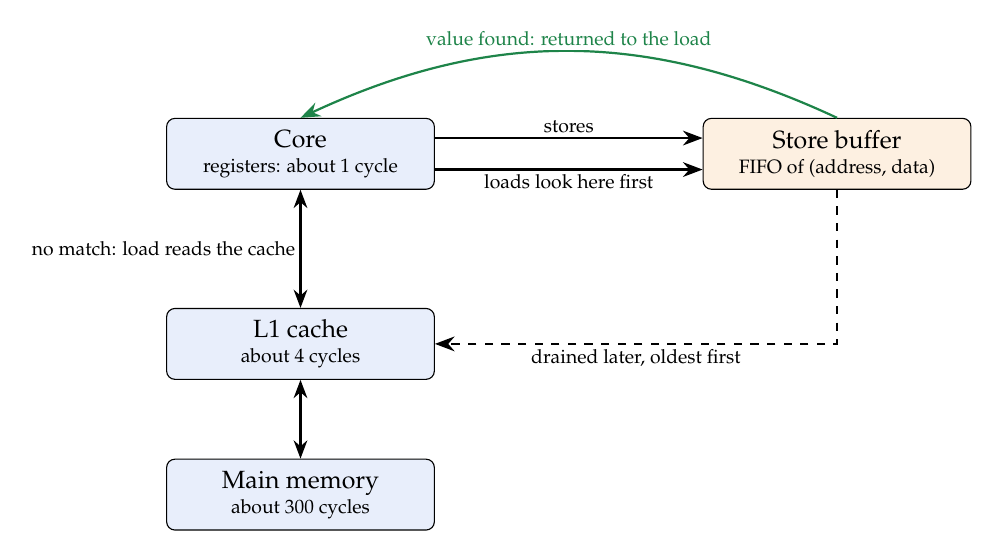
\begin{tikzpicture}[node distance=1.0cm, bx/.style={blk, minimum width=3.4cm}]
\node[bx] (core) {Core\\[-2pt]\scriptsize registers: about 1 cycle};
\node[bx, fill=boxorange, right=3.4cm of core] (sb) {Store buffer\\[-2pt]\scriptsize FIFO of (address, data)};
\node[bx, below=1.5cm of core] (l1) {L1 cache\\[-2pt]\scriptsize about 4 cycles};
\node[bx, below=1.0cm of l1] (mem) {Main memory\\[-2pt]\scriptsize about 300 cycles};
% stores go into the buffer
\draw[arr] ($(core.east)+(0,0.2)$) -- node[lab, above] {stores} ($(sb.west)+(0,0.2)$);
% a load looks in the buffer first
\draw[arr] ($(core.east)+(0,-0.2)$) -- node[lab, below] {loads look here first} ($(sb.west)+(0,-0.2)$);
% value found in the buffer comes straight back
\draw[arr, edgerf] (sb.north) to[bend right=25] node[lab, above] {value found: returned to the load} (core.north);
% no match in the buffer: the load goes to the cache, data comes back
\draw[arr, {Stealth}-{Stealth}] (core.south) -- node[lab, left] {no match: load reads the cache} (l1.north);
% the buffer drains into the cache
\draw[arr, dashed] (sb.south) |- node[lab, pos=0.75, below] {drained later, oldest first} (l1.east);
% cache and memory exchange data in both directions
\draw[arr, {Stealth}-{Stealth}] (l1.south) -- (mem.north);
\end{tikzpicture}
\caption{The memory path of one core (times from \cref{tab:latency}). A store goes into the store buffer and the core does not wait for it. A load first looks in the store buffer. If it finds a store to the same address there, it gets that value, and otherwise it reads the cache. Later the buffer drains into the cache, and the coherence protocol lets the other cores see the new value.}
\label{fig:sbpath}
\end{figure}

This is a large saving of time, and \cref{ch:cost} puts a number on it with a small model. This is also the source of the problem. After a store has left the core and entered the buffer, other cores cannot see it until the buffer drains. The store is finished as far as its own core is concerned, and it does not yet exist for everybody else.

Lamport's first requirement for sequential consistency, from \cref{sec:lamport}, was that each processor sends its memory requests in \gls{po}\cite{lamport1979}. A store buffer lets a later load reach memory before an earlier store does, so a machine with a store buffer gives up that requirement. Whether the program can tell is the question of the next two chapters.

\section{Store-to-load forwarding}
\label{sec:forwarding}

We start with a core that stores \code{x = 1} and then at once loads \code{x}. The new value is still in the store buffer and has not reached the cache. If the load simply read the cache it would get the old value, and the \emph{uniprocessor illusion}\index{uniprocessor illusion} would break. This is the rule that on a single core the result must be the same as if the program had run one instruction at a time, in order.

So every load first searches the store buffer. This is called \emph{\gls{fwd}}\index{store-to-load forwarding}, and it happens in the load-store queue of the core. \Cref{fig:forwarding} shows the circuit. There is one comparator for each buffer entry, which checks whether that entry's address equals the load's address. Several entries may match if the core wrote the same address more than once, and then a priority selector picks the youngest of the stores that come before the load. A multiplexer sends that entry's data to the load. If no entry matches, the load reads the cache.

\begin{figure}[!htbp]
\centering
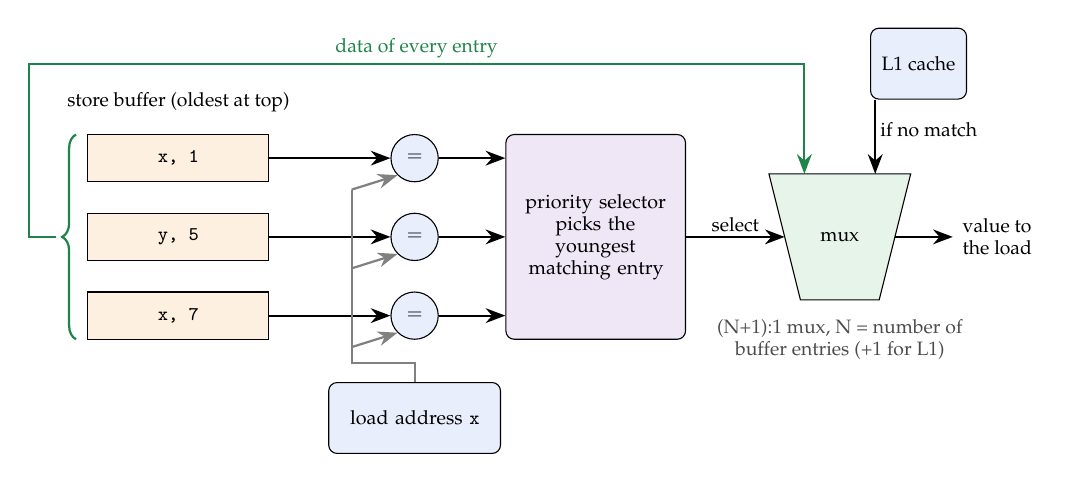
\begin{tikzpicture}[ent/.style={draw, fill=boxorange, minimum width=2.3cm, minimum height=0.6cm, font=\ttfamily\scriptsize},
  cmp/.style={draw, circle, fill=boxblue, inner sep=1pt, font=\scriptsize, minimum size=0.6cm}]
\foreach \i/\t in {0/{x, 1},1/{y, 5},2/{x, 7}} {
  \node[ent] (e\i) at (0,-\i*1.0) {\t};
  \node[cmp] (c\i) at (3.0,-\i*1.0) {$=$};
  \draw[arr] (e\i) -- (c\i);
}
\node[above=0.15cm of e0, font=\scriptsize] {store buffer (oldest at top)};
% load address bus
\node[blk, font=\scriptsize, text width=1.9cm] (la) at (3.0,-3.3) {load address \texttt{x}};
\draw[thick, gray] (la.north) -- (3.0,-2.6) -- (2.2,-2.6) -- (2.2,-0.4);
\foreach \i in {0,1,2} \draw[arr, gray] (2.2,-\i*1.0-0.4) -- (c\i.south west);
\node[blk, fill=boxpurple, text width=2.0cm, font=\scriptsize, minimum height=2.6cm] (pri) at (5.3,-1.0) {priority selector\\ picks the youngest matching entry};
\foreach \i in {0,1,2} \draw[arr] (c\i) -- (c\i -| pri.west);
% mux: wide side on top, two data inputs on top, select from the left
\draw[fill=boxgreen] (7.5,-0.2) -- (9.3,-0.2) -- (8.9,-1.8) -- (7.9,-1.8) -- cycle;
\node[font=\scriptsize] at (8.4,-1.0) {mux};
\node[font=\scriptsize, align=center, text=gray!60!black] at (8.4,-2.3) {(N+1):1 mux, N = number of\\ buffer entries (+1 for L1)};
\coordinate (inA) at (7.95,-0.2);
\coordinate (inB) at (8.85,-0.2);
\coordinate (muxw) at (7.7,-1.0);
\draw[arr] (pri.east) -- node[lab, above] {select} (muxw);
\node[blk, font=\scriptsize] (l1) at (9.4,1.2) {L1 cache};
\draw[arr] (l1.south -| inB) -- node[lab, right, pos=0.4] {if no match} (inB);
\node[font=\scriptsize, align=left] (out) at (10.4,-1.0) {value to\\ the load};
\draw[arr] (9.1,-1.0) -- (out);
% data of every entry: leaves the left side of each entry and goes to the mux
\draw[decorate, decoration={brace, amplitude=5pt, mirror}, thick, edgerf] (-1.3,0.3) -- (-1.3,-2.3);
\draw[arr, edgerf] (-1.55,-1.0) -- (-1.9,-1.0) -- (-1.9,1.2) -- node[lab, above, pos=0.5] {data of every entry} (inA |- 0,1.2) -- (inA);
\end{tikzpicture}
\caption{Store-to-load forwarding. Each entry compares its address with the load's address. Here two entries match \texttt{x}, and the selector picks the youngest one, so the load receives 7 from the buffer instead of the old value in the cache. The mux is drawn with two inputs for simplicity. In hardware it is an $(N{+}1)$-to-1 mux: one input for each of the $N$ buffer entries, plus one for the L1 cache.}
\label{fig:forwarding}
\end{figure}

Forwarding gives us the \emph{uniprocessor rule}: a load returns the value of the most recent earlier store to the same address in its own thread, if there is one. Every model in this paper obeys this rule. (This is the single-thread part of \emph{\gls{scl}}, \cref{sec:scloc}: if each address is checked on its own, a thread's own reads and writes of that address must never form a cycle. Forwarding is the hardware that keeps this true. \gls{sc} per location also asks that all threads agree on one order of the writes to an address, and that part comes from \gls{coh}.)

\section{What this means for two cores}
\label{sec:twocores}

Forwarding works only inside one core. A core always sees its own buffered stores. Other cores do not, because they read the shared cache and memory, and the buffered value has not arrived there yet (\cref{fig:twocores}).

\begin{figure}[!htbp]
\centering
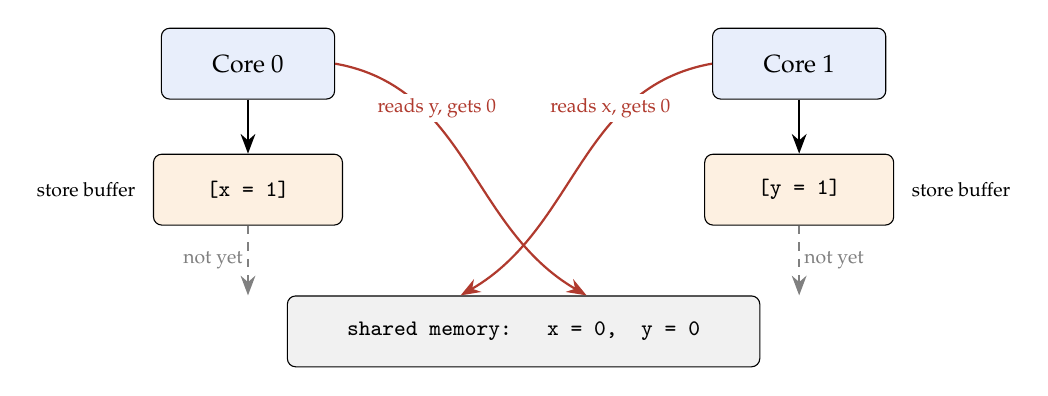
\begin{tikzpicture}
\node[blk, minimum width=2.2cm] (c0) at (0,0) {Core 0};
\node[blk, minimum width=2.2cm] (c1) at (7,0) {Core 1};
\node[blk, fill=boxorange, minimum width=2.4cm, font=\ttfamily\footnotesize] (b0) at (0,-1.6) {[x = 1]};
\node[blk, fill=boxorange, minimum width=2.4cm, font=\ttfamily\footnotesize] (b1) at (7,-1.6) {[y = 1]};
\node[font=\scriptsize, left=0.1cm of b0] {store buffer};
\node[font=\scriptsize, right=0.1cm of b1] {store buffer};
\node[blk, fill=boxgrey, minimum width=6cm, font=\ttfamily\footnotesize] (m) at (3.5,-3.4) {shared memory: \ x = 0, \ y = 0};
\draw[arr] (c0) -- (b0); \draw[arr] (c1) -- (b1);
\draw[arr, dashed, gray] (b0) -- node[lab, left] {not yet} (b0 |- m.north);
\draw[arr, dashed, gray] (b1) -- node[lab, right] {not yet} (b1 |- m.north);
\draw[arr, edgefr] (c0.east) to[out=-10, in=150] node[lab, pos=0.35, above] {reads y, gets 0} ($(m.north)+(0.8,0)$);
\draw[arr, edgefr] (c1.west) to[out=190, in=30] node[lab, pos=0.35, above] {reads x, gets 0} ($(m.north)+(-0.8,0)$);
\end{tikzpicture}
\caption{Each core sees its own buffered write, but not the other core's. While both writes wait in the buffers, both reads see the old values in memory.}
\label{fig:twocores}
\end{figure}

This difference between a core's own writes, which it sees at once, and another core's writes, which it sees only later, is exactly what lets two cores disagree about the order in which things happened. \Cref{ch:litmus} turns this picture into a concrete test.

\section{Cache coherence}
\label{sec:coherence}

Each core has its own private cache, so the same address can sit in several caches at once. If one core changes its copy, the others would keep reading a stale value. A \emph{coherence protocol}\index{cache coherence} prevents this by keeping all copies of an address in agreement. The usual one is \emph{MESI}\index{MESI}, named after the four states in which a cache line can be:

\begin{itemize}
  \item \textbf{Modified (M):} this cache holds the only copy, and it has been changed. Memory is out of date.
  \item \textbf{Exclusive (E):} this cache holds the only copy, and it is unchanged.
  \item \textbf{Shared (S):} several caches hold the same unchanged copy. Everyone may read it.
  \item \textbf{Invalid (I):} this cache's copy is out of date and must not be used.
\end{itemize}

The rule we need: before a core writes a line, every other cache must mark its copy Invalid. Only then does the writer get the line in the Modified state. A core that later reads that address misses in its own cache, and receives the new value from the writer.

Coherence therefore guarantees that all cores see the writes to the \emph{same} address in one agreed order. It says nothing about the order between writes to \emph{different} addresses. It also cannot see inside a store buffer, because a buffered store has not reached the cache yet. So even a perfectly coherent machine can show the surprising result of \cref{sec:intro-sb}. That is all we need from MESI.

\section{SC per location: the rule that never breaks}
\label{sec:scloc}

We look at one address, say \code{x}, and ignore all other variables. For that address alone, the machine behaves as if it were sequentially consistent:
\begin{itemize}
  \item all cores agree on one order of the writes to \code{x} (this comes from coherence);
  \item a thread's own reads and writes of \code{x} stay in program order (this comes from forwarding);
  \item every read of \code{x} returns a value that fits this order.
\end{itemize}
We call this \emph{SC per location}\index{SC per location}\cite{alglave2014}.

A small example: one thread does \code{x = 1; r = x;}. Even if \code{x = 1} is still in the store buffer, forwarding makes \code{r} equal to 1, never the old value 0.

\begin{notebox}
SC for one address does not mean SC for the whole program. Every surprise in this paper comes from a pair of operations on \emph{different} addresses.
\end{notebox}

% =====================================================================
\chapter{Two Cores: Shared Memory and Litmus Tests}
\label{ch:litmus}
% =====================================================================

We now put two cores next to each other with one shared memory, describe the three models in words, and use two \gls{litmus}s to see what each model allows.

\section{Operational Description of SC, TSO and PSO}
\label{sec:models-words}

Before the tests, here is how each of the three machines works in practice. Each one is a shared memory with two cores attached, and the only difference between them is what sits between a core and the memory.

\paragraph{SC (sequential consistency).} There is no \gls{sb}. When a core executes a store, the value goes straight into memory, and the very next load by any core sees it. Memory handles one operation at a time, and each core sends its operations in the order of its program. It behaves like a single shared notebook that the cores take turns writing in and reading from. This is the machine most people have in mind when they first write a parallel program, and it is the slowest, because a core must wait for memory on every store.

\paragraph{TSO (total store order).} Each core has \emph{one} store buffer, a queue where its stores wait before going to memory. A store joins the back of the queue, and the stores leave from the front, so a core's stores always reach memory in the order it issued them. A load first looks in its own core's buffer (\cref{sec:forwarding}) and takes the newest value for that address if it finds one. Otherwise it reads memory. The effect is that a core can run a load while its own earlier store is still waiting in the queue, so another core may read the old value for a short time. This is how x86 processors work.

\paragraph{PSO (partial store order).} Each core still has a store buffer, but it is looser. Stores to the \emph{same} address leave in the order they were issued, while stores to \emph{different} addresses may leave in any order. So a core that writes \code{x} and then \code{y} may find that \code{y} reaches memory first. A load still checks the core's own buffer first, as in \gls{tso}.

Programmers who need more order at one particular point can add a \gls{fence} instruction to their program. A full fence (\code{mfence}) makes the core wait until everything in its store buffer has reached memory before it goes on. A store fence (\code{stbar}) is lighter: it only makes sure that the stores written before it reach memory before the stores written after it.

\gls{sc} has no buffer, TSO has a queue, and \gls{pso} has a queue that can reorder stores to different addresses.

\section{Litmus tests}
\label{sec:notation}

A \emph{litmus test}\index{litmus test} is a tiny program of two threads, written to test one ordering rule. It always comes with one question: is this particular final result possible? The notation is the one set out in \cref{sec:conventions}: \code{x} and \code{y} are shared and start at 0, \code{r0} and \code{r1} are private registers, and threads T0 and T1 run on different cores.

This paper uses two litmus tests, Store Buffering (SB) and Message Passing (MP), and one fenced version of each.

\section{How many interleavings?}
\label{sec:interleave}

As we saw for SC, the machine should look as if a single processor did all the work, one operation at a time. Such a single timeline, which merges the instructions of the threads one after another, is called an \emph{interleaving}\index{interleaving}.

If thread A has $n_1$ instructions and thread B has $n_2$, an interleaving is fixed by choosing which $n_1$ of the $n_1+n_2$ time slots belong to A. The number of interleavings is therefore
\[
\binom{n_1+n_2}{n_1} \;=\; \frac{(n_1+n_2)!}{n_1!\;n_2!}.
\]
We keep in mind that the order of the instructions inside one thread can never be changed, so only the way the two threads are mixed together can differ. For two threads of two instructions each the count is $4!/(2!\,2!) = 6$. For three and three it is $6!/(3!\,3!) = 20$. To decide by brute force whether SC allows a result, we would have to try all of these orders.

\section{The Store Buffering test (SB)}
\label{sec:sb}

\begin{center}
\begin{tabular}{@{}l@{\hspace{1.5cm}}l@{}}
\toprule
T0 & T1\\
\midrule
\code{a: x = 1} & \code{c: y = 1}\\
\code{b: r0 = y} & \code{d: r1 = x}\\
\bottomrule
\end{tabular}
\end{center}

This is the program of \cref{sec:intro-sb}, with its four operations named $a$ to $d$. The question is whether we can end with \outc{0}{0}.

We first think the way a person would. Someone's write must come first, so the other thread's read should see it. \Cref{tab:sbinter} checks all six interleavings, keeping $a$ before $b$ and $c$ before $d$.

\begin{table}[!htbp]
\centering\small
\caption{The six interleavings of SB and the result each one gives.}
\label{tab:sbinter}
\begin{tabular}{@{}cc@{}}
\toprule
Order & Result $(\code{r0},\code{r1})$\\
\midrule
$a\,b\,c\,d$ & \outc{0}{1}\\
$a\,c\,b\,d$ & \outc{1}{1}\\
$a\,c\,d\,b$ & \outc{1}{1}\\
$c\,a\,b\,d$ & \outc{1}{1}\\
$c\,a\,d\,b$ & \outc{1}{1}\\
$c\,d\,a\,b$ & \outc{1}{0}\\
\bottomrule
\end{tabular}
\end{table}

When everything runs one operation at a time, the possible results are \outc{0}{1}, \outc{1}{1} and \outc{1}{0}. The result \outc{0}{0} never appears. Sequential consistency forbids it.

Now add store buffers. T0 puts \code{x = 1} in its buffer and carries on, so $b$ reads \code{y} from memory and gets 0. T1 puts \code{y = 1} in its buffer and carries on, so $d$ reads \code{x} from memory and gets 0. The buffers drain afterwards. The result is \outc{0}{0}, the outcome that cannot happen under SC. SB is therefore the test that separates SC from TSO: SC forbids \outc{0}{0}, while a machine with store buffers allows it. This is the central example of the paper.

\section{The Message Passing test (MP)}
\label{sec:mp}

\begin{center}
\begin{tabular}{@{}l@{\hspace{1.5cm}}l@{}}
\toprule
T0 & T1\\
\midrule
\code{a: x = 1} & \code{c: r0 = y}\\
\code{b: y = 1} & \code{d: r1 = x}\\
\bottomrule
\end{tabular}
\end{center}

Here \code{x} plays the part of some data and \code{y} the part of a flag that says the data is ready. T0 writes the data and then raises the flag. T1 reads the flag and then the data. The question is whether we can end with \outc{1}{0}, which would mean that T1 saw the flag raised but still read the old data. This pattern is behind every producer and consumer that pass work through memory, so a wrong answer here would break a lot of real programs.

Two different hardware features could produce \outc{1}{0}.
\begin{itemize}
\item The two writes of T0 become visible in the wrong order: \code{y = 1} reaches memory before \code{x = 1}.
\item The two reads of T1 run in the wrong order: \code{x} is read before \code{y}.
\end{itemize}
A store buffer that drains in FIFO order does neither. \code{x = 1} entered the buffer first, so it leaves first. The reads are not reordered at all. So TSO forbids \outc{1}{0}, and SC forbids it too. A store buffer that lets writes to different addresses leave in a different order would allow it, and that is the extra freedom of PSO. MP is therefore the test that separates TSO from PSO.

\section{What each model will say}
\label{sec:preview}

\Cref{tab:preview} is a preview of the answers. \Cref{ch:math} explains every cell with a graph, and \cref{ch:checker} confirms every cell with a program.

\begin{table}[!htbp]
\centering\small
\caption{Preview: is the named outcome of each test allowed? Explained in \cref{ch:math} and checked in \cref{ch:checker}.}
\label{tab:preview}
\begin{tabular}{@{}lccc@{}}
\toprule
Test and outcome & SC & TSO & PSO\\
\midrule
SB \outc{0}{0} & forbidden & allowed & allowed\\
MP \outc{1}{0} & forbidden & forbidden & allowed\\
\bottomrule
\end{tabular}
\end{table}

% =====================================================================
\chapter{SC, TSO and PSO: the Rules as Math}
\label{ch:math}
% =====================================================================

\noindent The description of \cref{ch:litmus} is easy to follow, but it is not precise enough to decide whether a given result is allowed. For that we need to say what each model permits.

\noindent We define the memory operations of a program and a few relations between them, state the rules a result must satisfy under each model, and draw the operations as points. We then work through four cases by hand, each with its own graph and its verdict. The same method is run by a program in \cref{ch:checker}.

\section{Events}
\label{sec:events}

Every memory instruction becomes an \emph{event}\index{event}: a read $R(\text{addr}, \text{value})$ or a write $W(\text{addr}, \text{value})$. In SB, $a$ is $W(x,1)$, $b$ is $R(y,?)$, $c$ is $W(y,1)$ and $d$ is $R(x,?)$. The question marks are the values we are asking about. We assume that the initial values are put in memory by \emph{initial writes}, $W(x,0)$ and $W(y,0)$, which happen before everything else. Each of them will act as a node in our graph later on.

\section{The four relations}
\label{sec:relations}

If the events are the nodes of a graph, then the relations are the directed edges between them. Each arrow has a meaning of its own: it records one logical fact about two events, such as that one must come before the other, or that one read its value from the other. In this way we are building a \emph{directed graph}\index{directed graph} of the program. A \emph{relation} is simply a set of such arrows, and we need four of them.

\begin{description}[leftmargin=0.9cm, style=nextline]
\item[\po\ \normalfont(program order)] An arrow $A \to B$ when $A$ comes before $B$ in the same thread. Program order\index{program order} never links instructions of two different threads.
\item[\rf\ \normalfont(reads-from)] An arrow $W \to R$ when the read $R$ returned the value written by $W$.
\item[\co\ \normalfont(coherence order)] For each address, the order in which its writes take effect, so it says which write to that address is \emph{later} in memory. The initial write always comes first.
\item[\fr\ \normalfont(from-read)] An arrow $R \to W'$ when $R$ read from some write $W$ and $W'$ comes after $W$ in \co. In words, $R$ saw an older value, so $R$ must have happened before the newer write $W'$. Formally \fr\ is \rf\ turned backwards and then followed by \co, written $\fr = \rf^{-1};\co$.
\end{description}

An \emph{execution}\index{execution} is one choice of \rf\ and \co: one story of which write every read got its value from, and in which order the writes to each address happened. Once \rf\ and \co\ are chosen, \fr\ follows from them, and the final values of the registers follow too.

\section{Acyclic means consistent}
\label{sec:acyclic}

The four relations above are the raw material. Each model uses them in a slightly modified form: it decides which of the arrows are kept, and in some cases in what shape. For example, a weaker model keeps only some of the program-order arrows (we will call these the \gls{ppo}, \ppo), and it counts a \gls{rf} arrow only when the value really travels between two different cores (the external reads-from, \rfe). The exact versions for each model are defined later in this chapter. Here we only need the method that is the same for all of them.

For a given program and a given result, we draw all the arrows that the model keeps as one directed graph. We read an arrow $A \to B$ as the statement that $A$ must happen before $B$. Then we look at the graph:
\begin{itemize}
  \item If the graph has a \emph{cycle}\index{cycle}, $A \to B \to \dots \to A$, the arrows would say that $A$ happens before itself. That is impossible, so no execution can produce this result, and the model \textbf{does not allow} it.
  \item If the graph has no cycle (it is \emph{acyclic}), the events can be placed on a single timeline in which every arrow points forward. Such a timeline is a possible execution that gives this result, so the model \textbf{allows} it.
\end{itemize}

\section{How the graphs in this chapter are drawn}
\label{sec:legend}

In every graph each operation is a small circle with a letter inside it. Before each graph we say which operation each letter stands for. The first thread is on the left with its first operation on top, the second thread is on the right, and the two initial writes sit above and below. Each kind of arrow has its own colour.
\begin{center}
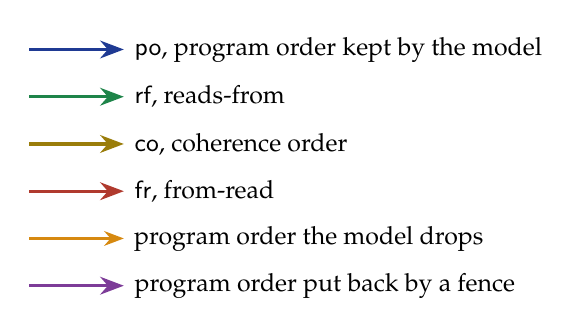
\begin{tikzpicture}
\draw[po] (0,0) -- (1.2,0) node[right, font=\small, text=black] {\po, program order kept by the model};
\draw[rf] (0,-0.6) -- (1.2,-0.6) node[right, font=\small, text=black] {\rf, reads-from};
\draw[co] (0,-1.2) -- (1.2,-1.2) node[right, font=\small, text=black] {\co, coherence order};
\draw[fr] (0,-1.8) -- (1.2,-1.8) node[right, font=\small, text=black] {\fr, from-read};
\draw[dropped] (0,-2.4) -- (1.2,-2.4) node[right, font=\small, text=black] {program order the model drops};
\draw[fenceedge] (0,-3.0) -- (1.2,-3.0) node[right, font=\small, text=black] {program order put back by a fence};
\end{tikzpicture}
\end{center}
The initial writes are kept as nodes of the graph, one for each variable, together with the arrows that leave them.

\section{The rules of each model}
\label{sec:rules}

All three models use the method of \cref{sec:acyclic}: draw the arrows the model keeps and look for a cycle. What changes from one model to the next is only which arrows are put in the graph. In this section we state the rule of each model in one place, and then explain every term in it.

\subsection{Notation used in the rules}

\begin{description}[leftmargin=0.9cm, style=nextline]
\item[\ppo\ \normalfont(preserved program order)\index{preserved program order}] The program-order arrows that the model still guarantees. We describe each program-order pair by the kinds of its two operations, first and second. \RR\ is a read followed by a read, \RW\ a read followed by a write, \WW\ a write followed by a write, and \WR\ a write followed by a read. The model decides which of these four pairs it keeps (\cref{tab:pairs}), and the pairs concern operations to \emph{different} addresses.
\item[\poloc\ \normalfont(program order on one address)] Program order restricted to pairs of operations on the \emph{same} address. No model drops these arrows.
\item[\rfe\ \normalfont(external reads-from)] The reads-from arrows between \emph{different} threads. A reads-from arrow inside one thread is not used in the global graph.
\end{description}

\begin{table}[!htbp]
\centering\small
\caption{Which program-order pairs each model keeps, for operations to different addresses in the same thread. This table is the whole definition of each model in our checker.}
\label{tab:pairs}
\begin{tabular}{@{}lccc@{}}
\toprule
Pair (first $\to$ second) & SC & TSO & PSO\\
\midrule
\RR & kept & kept & kept\\
\RW & kept & kept & kept\\
\WW & kept & kept & \textbf{dropped}\\
\WR & kept & \textbf{dropped} & \textbf{dropped}\\
\bottomrule
\end{tabular}
\end{table}

Reading the table from left to right, each step drops one more kind of arrow.

\subsection{Fences}
\label{sec:fencedef}

A \emph{\gls{fence}}\index{fence} is an instruction that says that the memory operations of this thread before it must be ordered before the ones after it. In the graph, a fence adds back the dropped arrows between operations on either side of it. Different fences put back different pairs (\cref{tab:fences}).

\begin{table}[!htbp]
\centering\small
\caption{The two fences used in this paper and the arrows they put back.}
\label{tab:fences}
\begin{tabularx}{\textwidth}{@{}lXl@{}}
\toprule
Fence & Puts back & Used for\\
\midrule
full fence (x86 \code{mfence}) & all four pairs, including \WR & the fence SB needs\\
store-store fence (SPARC \code{stbar}) & \WW\ only & the writer side of MP under PSO\\
\bottomrule
\end{tabularx}
\end{table}

\subsection{The rules}

\begin{notebox}
\textbf{SC.} Every program-order pair is kept. \gls{sc} allows an execution if and only if the graph $\po \cup \rf \cup \co \cup \fr$ has no cycle.
\end{notebox}

\begin{notebox}
\textbf{TSO and PSO.} The model allows an execution if and only if
\begin{enumerate}[label=(\roman*)]
\item the graph $\ppo \cup \text{fences} \cup \rfe \cup \co \cup \fr$ has no cycle, and
\item the graph $\poloc \cup \rf \cup \co \cup \fr$ has no cycle.
\end{enumerate}
For \gls{tso}, \ppo\ contains \RR, \RW\ and \WW. For \gls{pso}, \ppo\ contains only \RR\ and \RW.
\end{notebox}

The symbol $\cup$ just means that we put all these arrows into the same graph. The two conditions have different jobs. Condition (i) looks at all addresses together, and it uses only the program-order arrows that the model keeps. Condition (ii) looks at each address on its own, and it is the \gls{scl} rule of \cref{sec:scloc}, which is the same in every model.

\section{The Store Buffering test (SB)}
\label{sec:sbgraph}

We now take the two \gls{litmus}s one by one and build their graphs under each model. The first is SB (\cref{sec:sb}), with the outcome \outc{0}{0}. Every operation becomes a circle, and the letter inside it is the name of the operation:
\begin{itemize}
\item[\textbf{a}] $W(x,1)$: T0 writes 1 to \code{x}.
\item[\textbf{b}] $R(y,0)$: T0 reads \code{y} and gets 0.
\item[\textbf{c}] $W(y,1)$: T1 writes 1 to \code{y}.
\item[\textbf{d}] $R(x,0)$: T1 reads \code{x} and gets 0.
\item[\textbf{e}] $W(x,0)$: the initial write of \code{x}.
\item[\textbf{f}] $W(y,0)$: the initial write of \code{y}.
\end{itemize}
The result fixes all the arrows except the program-order ones, which depend on the model. Since $b$ read 0, it read from the initial write $f$, and since $d$ read 0, it read from $e$. The initial writes come first in \co, so $e \to a$ and $f \to c$. Finally, $b$ read from $f$ and $c$ is a later write to \code{y}, so $b \to c$ by \fr. In the same way $d \to a$.

\subsection{SB under SC}
\label{sec:sbsc}

SC keeps both program-order arrows, $a \to b$ and $c \to d$. We add the arrows in four steps (\cref{fig:sbsc}): first all the program-order arrows, then the reads-from arrows, then the coherence arrows, and finally the \gls{fr} arrows.

\begin{figure}[H]
\centering
\fourpanels{\sbpanel}{1}{cyc}
\caption{SB with result \outc{0}{0} under SC, built step by step. After the last step the arrows $a \to b \to c \to d \to a$ close a cycle.}
\label{fig:sbsc}
\end{figure}

\begin{forbidbox}{Result: SB \outc{0}{0} under SC is forbidden}
The graph has the cycle $a \to b \to c \to d \to a$, so no single timeline can explain this result. This one argument replaces the whole table of six interleavings in \cref{tab:sbinter}.
\end{forbidbox}

\subsection{SB under TSO}
\label{sec:tso}
\label{sec:sbtso}

Total Store Order drops exactly one kind of pair, \WR. A later read may come before an earlier write to a different address in the order of the model. All other pairs are kept.

In SB, $a \to b$ is a write followed by a read of a different address, so TSO drops it, and the same holds for $c \to d$. We build the graph in the same four steps (\cref{fig:sbtso}). The two dropped arrows are shown in orange in the first step only.

\begin{figure}[H]
\centering
\fourpanels{\sbpanel}{0}{no cycle}
\caption{SB with result \outc{0}{0} under TSO, built step by step. The two write-then-read arrows are dropped, so no cycle can form.}
\label{fig:sbtso}
\end{figure}

\begin{resultbox}{Result: SB \outc{0}{0} under TSO is allowed}
With the two \WR\ arrows gone, the cycle of the SC graph is broken. The remaining arrows fit on one timeline, for example $e, f, b, d, a, c$. The same mathematics with one arrow kind fewer explains the surprise.
\end{resultbox}

\subsection{SB under PSO}
\label{sec:pso}

Partial Store Order drops \WW\ pairs to different addresses as well. PSO therefore allows everything TSO allows, plus one more reordering. SB has only \WR\ pairs, so the graph is exactly the one of TSO (\cref{fig:sbpso}).

\begin{figure}[H]
\centering
\fourpanels{\sbpanel}{0}{no cycle}
\caption{SB with result \outc{0}{0} under PSO. The graph is the same as under TSO, because SB contains no write-then-write pair.}
\label{fig:sbpso}
\end{figure}

\begin{resultbox}{Result: SB \outc{0}{0} under PSO is allowed}
The write-then-read arrows are dropped, so there is no cycle, exactly as under TSO.
\end{resultbox}

\section{The Message Passing test (MP)}
\label{sec:mpgraph}

The second test is MP (\cref{sec:mp}), with the outcome \outc{1}{0}. The letters stand for the following operations:
\begin{itemize}
\item[\textbf{a}] $W(x,1)$: T0 writes the data \code{x}.
\item[\textbf{b}] $W(y,1)$: T0 writes the flag \code{y}.
\item[\textbf{c}] $R(y,1)$: T1 reads the flag and gets 1.
\item[\textbf{d}] $R(x,0)$: T1 reads the data and gets 0.
\item[\textbf{e}] $W(x,0)$: the initial write of \code{x}.
\item[\textbf{f}] $W(y,0)$: the initial write of \code{y}.
\end{itemize}
The result fixes these arrows: $c$ read the 1 written by $b$, so $b \to c$ by \rf, and $d$ read the initial 0, so $e \to d$ by \rf. The initial writes come first in \co, so $e \to a$ and $f \to b$. Since $d$ read from $e$ and $a$ is a later write to \code{x}, $d \to a$ by \fr. The program-order arrows $a \to b$ (a \WW\ pair) and $c \to d$ (a \RR\ pair) depend on the model.

\subsection{MP under SC}
\label{sec:mpsc}

SC keeps both program-order arrows (\cref{fig:mpsc}).

\begin{figure}[H]
\centering
\fourpanels{\mppanel}{1}{cyc}
\caption{MP with result \outc{1}{0} under SC, built step by step. The arrows $a \to b \to c \to d \to a$ close a cycle.}
\label{fig:mpsc}
\end{figure}

\begin{forbidbox}{Result: MP \outc{1}{0} under SC is forbidden}
The graph has the cycle $a \to b \to c \to d \to a$. In words, a reader that sees the flag must also see the data.
\end{forbidbox}

\subsection{MP under TSO}
\label{sec:mptso}

TSO drops only \WR\ pairs. MP has a \WW\ pair and a \RR\ pair, and TSO keeps both, so the graph is the same as under SC (\cref{fig:mptso}).

\begin{figure}[H]
\centering
\fourpanels{\mppanel}{1}{cyc}
\caption{MP with result \outc{1}{0} under TSO. Both program-order arrows are kept, so the graph is the one of SC and the cycle is still there.}
\label{fig:mptso}
\end{figure}

\begin{forbidbox}{Result: MP \outc{1}{0} under TSO is forbidden}
All the arrows exist and $a \to b \to c \to d \to a$ is a cycle.
\end{forbidbox}

\subsection{MP under PSO}
\label{sec:mppso}

PSO also drops \WW\ pairs to different addresses, so $a \to b$ is dropped. The \RR\ pair $c \to d$ is still kept (\cref{fig:mppso}).

\begin{figure}[H]
\centering
\fourpanels{\mppanel}{0}{no cycle}
\caption{MP with result \outc{1}{0} under PSO, built step by step. The write-then-write arrow is dropped, and what remains is a chain with a start and an end.}
\label{fig:mppso}
\end{figure}

\begin{resultbox}{Result: MP \outc{1}{0} under PSO is allowed}
Without $a \to b$ the arrows form the chain $f \to b \to c \to d \to a$ (with $e$ before $a$ and $d$), which has no cycle.
\end{resultbox}

\section{Fences in the examples}
\label{sec:fences}

We now return to the two tests that needed a fence. A fence is not a node, because it is not a read or a write. It only adds a purple arrow between the two operations on either side of it, and the rest of the graph is built as before.

\subsection{SB with a fence in each thread, under TSO}

We put \code{mfence} between $a$ and $b$ and between $c$ and $d$. The nodes are the same as in \cref{sec:sbgraph}. Each fence puts back the \WR\ arrow that TSO had dropped, and we build the graph in the same four steps (\cref{fig:sbfence}).

\begin{figure}[H]
\centering
\fourpanels{\sbpanel}{2}{cyc}
\caption{SB with \texttt{mfence} in both threads, result \outc{0}{0}, under TSO, built step by step. The fences put back the two arrows that TSO dropped, and the cycle of the SC graph returns.}
\label{fig:sbfence}
\end{figure}

\begin{forbidbox}{Result: SB with mfence in both threads, \outc{0}{0} under TSO is forbidden}
The fences restore $a \to b$ and $c \to d$, and $a \to b \to c \to d \to a$ is a cycle again.
\end{forbidbox}

One fence alone is not enough. With a fence only in T0, the arrow $c \to d$ is still missing, the remaining arrows form the chain $d \to a \to b \to c$, and \outc{0}{0} stays allowed.

\subsection{MP with a store-store fence on the writer, under PSO}

We put \code{stbar} between $a$ and $b$ in T0. It puts back the \WW\ arrow that PSO had dropped. T1 needs no fence, because PSO already keeps \RR. The nodes are the same as in \cref{sec:mpgraph} (\cref{fig:mpfence}).

\begin{figure}[H]
\centering
\fourpanels{\mppanel}{2}{cyc}
\caption{MP with a store-store fence in T0, result \outc{1}{0}, under PSO, built step by step. The fence puts back the arrow that PSO dropped, and the cycle returns.}
\label{fig:mpfence}
\end{figure}

\begin{forbidbox}{Result: MP with stbar in T0, \outc{1}{0} under PSO is forbidden}
With $a \to b$ restored, the cycle $a \to b \to c \to d \to a$ returns. The fence keeps the write of the data ahead of the write of the flag, and that is all PSO needs.
\end{forbidbox}

\section{The ladder, and how to show it is strict}
\label{sec:ladder}

Each model keeps a subset of the arrows of the model above it in \cref{tab:pairs}. Removing arrows from a graph can break a cycle but can never create one. So every execution that SC allows, TSO also allows, and every execution TSO allows, PSO also allows:
\[
\text{allowed}(\text{SC}) \;\subseteq\; \text{allowed}(\text{TSO}) \;\subseteq\; \text{allowed}(\text{PSO}).
\]
The second rule, SC per location, is the same in all three models, so it does not upset this argument.

To show that each step is strict, it is enough to find one test that the weaker model allows and the stronger one forbids. The two tests above give both witnesses (\cref{tab:witness}), and \cref{fig:nested} draws the result.

\begin{table}[!htbp]
\centering\small
\caption{The test that separates each pair of neighbouring models.}
\label{tab:witness}
\begin{tabular}{@{}lll@{}}
\toprule
Step & Test that separates them & Reason\\
\midrule
SC vs TSO & SB, outcome \outc{0}{0} & \WR\ dropped\\
TSO vs PSO & MP, outcome \outc{1}{0} & \WW\ dropped\\
\bottomrule
\end{tabular}
\end{table}

\begin{figure}[H]
\centering
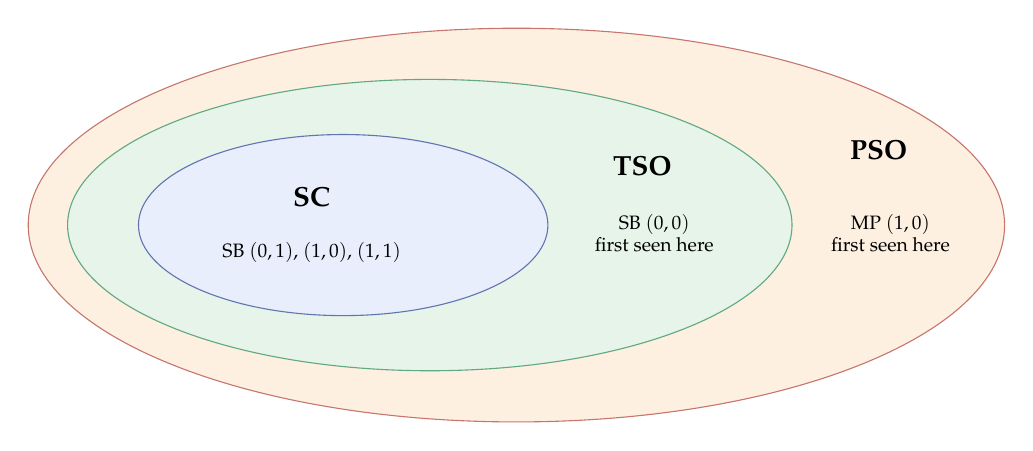
\begin{tikzpicture}
\draw[fill=boxorange, draw=edgefr!70] (0,0) ellipse (6.2cm and 2.5cm);
\draw[fill=boxgreen, draw=edgerf!70] (-1.1,0) ellipse (4.6cm and 1.85cm);
\draw[fill=boxblue, draw=edgepo!70] (-2.2,0) ellipse (2.6cm and 1.15cm);
\node[font=\bfseries] at (-2.6,0.35) {SC};
\node[font=\scriptsize, align=center] at (-2.6,-0.35) {SB \outc{0}{1}, \outc{1}{0}, \outc{1}{1}};
\node[font=\bfseries] at (1.6,0.75) {TSO};
\node[font=\scriptsize, align=center] at (1.75,-0.1) {SB \outc{0}{0}\\ first seen here};
\node[font=\bfseries] at (4.6,0.95) {PSO};
\node[font=\scriptsize, align=center] at (4.75,-0.1) {MP \outc{1}{0}\\ first seen here};
\end{tikzpicture}
\caption{The three models as nested sets of allowed outcomes.}
\label{fig:nested}
\end{figure}

\section{From hand-built graphs to a program}
\label{sec:towards}

In this chapter we followed one method for every model and every test. We turn each operation into a node, add the arrows that the model keeps, and look for a cycle. By hand this took one four-step figure for each pair of test and model, which is already a lot of drawing for two tiny tests. A larger program, or a model with more rules, would be far too long to do by hand.

The method itself is mechanical. Every step is a clear rule: list the events, add the arrows of the four relations, drop the program-order pairs that the model does not keep, add the arrows that fences put back, and test the graph for a cycle. A program can do all of this. In \cref{ch:checker} we write that program, run it on our litmus tests under all three models, and compare its answers with the verdicts we reached by hand. Those hand-made verdicts are our predictions.

% =====================================================================
\chapter{Experiment 1: the Python Checker (Q1)}
\label{ch:checker}
% =====================================================================

In \cref{ch:math} we reached our results by working through a few examples by hand, and we also want to verify these results empirically. For this we turn the same method into a program, the checker. It does what \cref{ch:math} describes, only mechanically. This chapter shows how the code is split into files, how each file works, what the checker prints, and how we check the checker itself, first with random programs and then with a second program that simulates the \gls{sb}s directly. All the programs are listed in full in \cref{app:code}.

\section{The files}
\label{sec:files}

The code has one clear split. Building the graph of a program is the job of the \emph{model} files, one for each model, and the checker only does the checking: it lists the guesses, looks for cycles and collects the outcomes. The checker just asks the model for its graphs (\cref{tab:checkfiles}). The simulation of \cref{sec:sim} is a seventh file that comes after these six.

\begin{table}[!htbp]
\centering\small
\caption{The files of the checker.}
\label{tab:checkfiles}
\begin{tabularx}{\textwidth}{@{}lX@{}}
\toprule
File & What it contains\\
\midrule
\code{tests.py} & the five litmus tests, the outcome we ask about in each, the expected answers, and 2000 random programs\\
\code{graph.py} & small helpers that build kinds of arrows, shared by the model files\\
\code{sc.py} & the model SC: how its graph is built\\
\code{tso.py} & the model TSO: how its graphs are built\\
\code{pso.py} & the model PSO: how its graphs are built\\
\code{checker.py} & the checker: events, guesses, cycle detection, outcomes and printing\\
\bottomrule
\end{tabularx}
\end{table}

Running \code{python3 checker.py} prints the verdict for each \gls{litmus}, the candidate executions of SB and MP, and the result of the subset check on all 2005 programs. It takes about one second.

\section{The test programs: \texttt{tests.py}}
\label{sec:testsfile}

The file \code{tests.py} holds every program that we give to the checker. We first write a few tests by hand, and then we add 2000 random tests that were generated with the help of an LLM. The hand-written tests are small and we know their answers in advance, so they show that the checker agrees with \cref{ch:math}. The random tests are many and varied, so they check that the checker is right on programs that we did not think of ourselves.

A program is a list of threads, and a thread is a list of instructions. For example, \code{("W", "x", 1)} is a write that writes the value 1 to the address \code{x}, \code{("R", "r0", "y")} is a read that reads the address \code{y} into the register \code{r0}, and \code{("F", "mfence")} is a \gls{fence}. The other fence is \code{("F", "stbar")}.

\paragraph{Five hand-written litmus tests.} These are SB, SB with \code{mfence} in both threads, MP, MP with \code{stbar} in the writer, and OwnWrite, the single-thread test of \cref{sec:scloc}. They are stored in the dictionary \code{LITMUS}. For each test the file keeps two more things.
\begin{itemize}
\item \code{TARGET} is the outcome we ask about, for example both reads return 0 in SB.
\item \code{EXPECTED} is the answer we expect for \gls{sc}, \gls{tso} and \gls{pso}, written as three letters, where \code{A} means allowed and \code{F} means forbidden.
\end{itemize}
The expected answers are the predictions of \cref{ch:math}. We wrote them down before running the checker.

\begin{figure}[!htbp]
\centering
\begin{lstlisting}[style=vspython]
# ---- the 5 hand-written litmus tests ---------------------------------
LITMUS = {
    "SB":         [[("W", "x", 1), ("R", "r0", "y")],
                   [("W", "y", 1), ("R", "r1", "x")]],
    "SB+mfences": [[("W", "x", 1), ("F", "mfence"), ("R", "r0", "y")],
                   [("W", "y", 1), ("F", "mfence"), ("R", "r1", "x")]],
    "MP":         [[("W", "x", 1), ("W", "y", 1)],
                   [("R", "r0", "y"), ("R", "r1", "x")]],
    "MP+stbar":   [[("W", "x", 1), ("F", "stbar"), ("W", "y", 1)],
                   [("R", "r0", "y"), ("R", "r1", "x")]],
    "OwnWrite":   [[("W", "x", 1), ("R", "r0", "x")]],
}

# The outcome each litmus test asks about.
TARGET = {
    "SB": {"r0": 0, "r1": 0},      "SB+mfences": {"r0": 0, "r1": 0},
    "MP": {"r0": 1, "r1": 0},      "MP+stbar":   {"r0": 1, "r1": 0},
    "OwnWrite": {"r0": 0},
}

# Expected answer for (SC, TSO, PSO): A = allowed, F = forbidden.
EXPECTED = {
    "SB": "FAA", "SB+mfences": "FFF", "MP": "FFA",
    "MP+stbar": "FFF", "OwnWrite": "FFF",
}
\end{lstlisting}
\caption{The litmus tests, the outcome asked about in each test, and the expected answers, as written in \code{tests.py}.}
\label{fig:testscode}
\end{figure}

\paragraph{Two thousand random programs.} These are stored in the list \code{RANDOM\_TESTS}. Each program has two threads of one to three instructions, chosen from writes, reads and the two fences over the addresses \code{x} and \code{y}. They were generated with the help of an LLM, and we saved them in the file, so every run of the checker and of the simulation uses exactly the same programs. For these programs we do not know the answers beforehand. Instead we compare the models with each other and with the simulation of \cref{sec:sim}. Together with the five litmus tests this gives 2005 programs.

\section{Building the arrows: \texttt{graph.py}}
\label{sec:graphfile}

An arrow is a pair of events $(A, B)$ and means that $A$ must happen before $B$. The file \code{graph.py} has one small function for each kind of arrow that \cref{ch:math} uses (\cref{tab:grapher}).

\begin{table}[!htbp]
\centering\small
\caption{The functions of \code{graph.py}.}
\label{tab:grapher}
\begin{tabularx}{\textwidth}{@{}lX@{}}
\toprule
Function & Arrows it builds\\
\midrule
\code{program\_order} & every pair of operations of one thread, earlier first\\
\code{preserved\_program\_order} & the program-order arrows that a model keeps, given the set of pairs it keeps (the ppo of \cref{sec:rules})\\
\code{fence\_arrows} & the arrows that fences put back\\
\code{external\_reads\_from} & the reads-from arrows between different threads (the rfe)\\
\code{from\_read\_arrows} & the from-read arrows, worked out from reads-from and the write order\\
\code{same\_address\_arrows} & the graph of one address at a time: program order on one address, reads-from, write order and from-read\\
\bottomrule
\end{tabularx}
\end{table}

The set of kept pairs is written with two letters for each pair, the kind of the first operation and the kind of the second. For example \code{"WR"} is a write followed by a read.

\section{The three models: \texttt{sc.py}, \texttt{tso.py}, \texttt{pso.py}}
\label{sec:modeltable}

Each model file has one function, \code{graphs}. It takes the events, the fences and one guess of an execution (its \gls{rf}, \rf, and its \gls{co}, \co), and it returns the list of graphs that must all have no cycle. The function is the rule of \cref{sec:rules}, written in Python. For SC the rule is one graph, with every program-order arrow in it.

\begin{figure}[!htbp]
\centering
\begin{lstlisting}[style=vspython]
"""SC keeps every program-order pair."""
from graph import program_order, from_read_arrows


def graphs(events, fences, reads_from, write_order):
    arrows = (program_order(events) + reads_from + write_order
              + from_read_arrows(reads_from, write_order))
    
    return [arrows]
\end{lstlisting}
\caption{The model file \code{sc.py}.}
\label{fig:sccode}
\end{figure}

For TSO and PSO the rule has two graphs: the global graph, with the \gls{ppo}, the fence arrows and only the external reads-from, and the graph of one address at a time. The two files are the same except for the set of pairs they keep.

\begin{figure}[!htbp]
\centering
\begin{lstlisting}[style=vspython]
"""TSO relaxes W -> R because of the store buffer."""
from graph import (preserved_program_order, fence_arrows, external_reads_from,
                   from_read_arrows, same_address_arrows)

KEPT = {"RR", "RW", "WW"}


def graphs(events, fences, reads_from, write_order):
    global_arrows = (preserved_program_order(events, KEPT)
                     + fence_arrows(events, fences)
                     + external_reads_from(reads_from)
                     + write_order
                     + from_read_arrows(reads_from, write_order))
    
    return [global_arrows, same_address_arrows(events, reads_from, write_order)]
\end{lstlisting}
\caption{The model file \code{tso.py}. The file \code{pso.py} is the same, with \code{KEPT = \{"RR", "RW"\}}.}
\label{fig:tsocode}
\end{figure}

Adding a model is one new file of this kind, and the checker does not change. This is the benefit of keeping the graph building apart from the checking.

\section{How \texttt{checker.py} works}
\label{sec:algo}

The checker follows five steps. \Cref{tab:checksteps} shows which function does each of them. Step 3 is done outside the checker, by the model file.

\begin{table}[!htbp]
\centering\small
\caption{The steps of the checker and the functions that do them.}
\label{tab:checksteps}
\begin{tabularx}{\textwidth}{@{}lXl@{}}
\toprule
Step & What happens & Function\\
\midrule
1 & every read and write of the program becomes an event, and every address gets an initial write & \code{make\_events}\\
2 & we guess an execution: for each read, which write it reads from, and for each address, the order of its writes & \code{all\_guesses}\\
3 & the model builds the arrows of the guess & \code{graphs} of the model file\\
4 & we look for a cycle in each graph & \code{has\_cycle}\\
5 & the outcome of every guess without a cycle is an allowed outcome & \code{guess\_is\_possible}, \code{check}\\
\bottomrule
\end{tabularx}
\end{table}

\paragraph{Step 1: events.} Each read and each write becomes an \code{Event} that remembers its kind, its address, its value or register, its thread and its position inside the thread. We name the events $a$, $b$, $c, \dots$ in order. The initial writes belong to no thread. Fences are not events. They are kept in a separate list, exactly because a fence is not a read or a write.

\paragraph{Step 2: guesses.} A \emph{guess} chooses the \rf\ of every read and the \co\ of every address. For the \rf, each read tries every write to its own address. For the \co, the initial write stays first and the other writes of the address come in every possible order. Every combination of these choices is one guess. For SB this gives $2 \times 2 = 4$ guesses, and the same for MP.

\paragraph{Step 4: cycles.} A directed graph has a cycle if and only if it cannot be put in a \emph{topological order}, an order in which every arrow points forwards. Our function uses Kahn's method: keep removing a node that has no incoming arrows. If every node can be removed, there is no cycle. If some nodes can never be removed, they are stuck in a cycle. Our graphs have between three and eight nodes, so this takes no measurable time.

\paragraph{Step 5: decision.} A guess is possible under a model if none of the graphs that the model returns has a cycle. The outcome of a guess is the final value of each register and of each address, and \code{check} collects the outcomes of all possible guesses.

\begin{figure}[!htbp]
\centering
\begin{lstlisting}[style=vspython]
def check(test, model):
    events, fences, var_list = make_events(test)
    allowed = set()

    for guess in all_guesses(events, var_list):
        if guess_is_possible(events, fences, model, guess):
            allowed.add(outcome_of(guess))

    return allowed
\end{lstlisting}
\caption{The function \code{check} of \code{checker.py}.}
\label{fig:checkcode}
\end{figure}

\section{What the checker prints}
\label{sec:checkres}

The checker prints three things. The first is the verdict on the named outcome of each litmus test (\cref{tab:verdicts}), next to the prediction from \cref{ch:math}.

\begin{table}[!htbp]
\centering\small
\caption{Checker verdicts on the named outcome of each test. A means allowed and F means forbidden. Every verdict matches the prediction of \cref{ch:math}.}
\label{tab:verdicts}
\begin{tabular}{@{}llcccc@{}}
\toprule
Test & Outcome & SC & TSO & PSO & Matches prediction\\
\midrule
SB & \outc{0}{0} & F & A & A & yes\\
SB+mfences & \outc{0}{0} & F & F & F & yes\\
MP & \outc{1}{0} & F & F & A & yes\\
MP+stbar & \outc{1}{0} & F & F & F & yes\\
OwnWrite & $\code{r0}=0$ & F & F & F & yes\\
\bottomrule
\end{tabular}
\end{table}

The second is the list of all candidate executions of SB and MP, with the verdict of each model. In SB, read $b$ can take its value from the initial write of \code{y} or from $c$, and read $d$ from the initial write of \code{x} or from $a$, so there are four guesses (\cref{tab:candsb}). Each address has only one write besides its initial write, so the coherence order has no other choice. MP also has four guesses (\cref{tab:candmp}).

For SB, SC allows three outcomes, and TSO and PSO allow all four. The first row is SB under the three models from \cref{sec:sbgraph}, now found by the program. For MP, only the outcome \outc{1}{0} changes between the models: SC and TSO allow three outcomes and PSO allows four. The third row is MP under the three models from \cref{sec:mpgraph}.

\begin{table}[!htbp]
\centering\small
\caption{The four candidate executions of SB, as printed by the checker. \emph{cycle} means the model rejects the candidate.}
\label{tab:candsb}
\begin{tabular}{@{}lcccc@{}}
\toprule
Choice of \rf & $(\code{r0},\code{r1})$ & SC & TSO & PSO\\
\midrule
$b$ reads initial \code{y}, $d$ reads initial \code{x} & \outc{0}{0} & cycle & allowed & allowed\\
$b$ reads initial \code{y}, $d$ reads $a$ & \outc{0}{1} & allowed & allowed & allowed\\
$b$ reads $c$, $d$ reads initial \code{x} & \outc{1}{0} & allowed & allowed & allowed\\
$b$ reads $c$, $d$ reads $a$ & \outc{1}{1} & allowed & allowed & allowed\\
\bottomrule
\end{tabular}
\end{table}

\begin{table}[!htbp]
\centering\small
\caption{The four candidate executions of MP, as printed by the checker.}
\label{tab:candmp}
\begin{tabular}{@{}lcccc@{}}
\toprule
Choice of \rf & $(\code{r0},\code{r1})$ & SC & TSO & PSO\\
\midrule
$c$ reads initial \code{y}, $d$ reads initial \code{x} & \outc{0}{0} & allowed & allowed & allowed\\
$c$ reads initial \code{y}, $d$ reads $a$ & \outc{0}{1} & allowed & allowed & allowed\\
$c$ reads $b$, $d$ reads initial \code{x} & \outc{1}{0} & cycle & cycle & allowed\\
$c$ reads $b$, $d$ reads $a$ & \outc{1}{1} & allowed & allowed & allowed\\
\bottomrule
\end{tabular}
\end{table}

The third is the subset check, which we describe in \cref{sec:sanity}. For every program, the checker can also list all the outcomes that each model allows (\cref{tab:outcomes}). Adding a fence removes exactly the outcome that the model had added.

\begin{table}[!htbp]
\centering\small
\caption{All allowed register outcomes $(\code{r0},\code{r1})$ of the litmus tests, computed by the checker.}
\label{tab:outcomes}
\begin{tabular}{@{}llc l@{}}
\toprule
Test & Model & Count & Allowed outcomes\\
\midrule
SB & SC & 3 & \outc{0}{1} \outc{1}{0} \outc{1}{1}\\
SB & TSO, PSO & 4 & \outc{0}{0} \outc{0}{1} \outc{1}{0} \outc{1}{1}\\
SB+mfences & SC, TSO, PSO & 3 & \outc{0}{1} \outc{1}{0} \outc{1}{1}\\
MP & SC, TSO & 3 & \outc{0}{0} \outc{0}{1} \outc{1}{1}\\
MP & PSO & 4 & \outc{0}{0} \outc{0}{1} \outc{1}{0} \outc{1}{1}\\
MP+stbar & SC, TSO, PSO & 3 & \outc{0}{0} \outc{0}{1} \outc{1}{1}\\
OwnWrite & SC, TSO, PSO & 1 & $\code{r0} = 1$\\
\bottomrule
\end{tabular}
\end{table}

We also asked the checker about SB with a fence in T0 only. It allows \outc{0}{0} under TSO and PSO, as \cref{sec:fences} argued: one fence is not enough for SB.

\section{Understanding the results of the checker}
\label{sec:sanity}

\Cref{fig:checkout} shows what \code{python checker.py} prints. The output has three parts, one after the other, and a checker is only useful if we can read them correctly, so we go through each part here.

\paragraph{The verdicts.} Each row of the first part is one litmus test. The columns give the outcome that we asked about, the verdict of SC, TSO and PSO (\code{A} for allowed and \code{F} for forbidden), and whether this matches the answer that we stored in \code{EXPECTED}. SB is allowed under TSO and PSO and forbidden under SC. MP is allowed only under PSO. SB with \code{mfence} and MP with \code{stbar} are forbidden under all three models, so a fence removes exactly the outcome that the weaker models had added. OwnWrite is forbidden under all three models, because the graph of one address catches it. Every row says \code{yes} in the last column, so the checker gives the same answers that we worked out by hand in \cref{ch:math}. The verdicts on SB and MP for SC and TSO are also standard results\cite{owens2009}, so if our code had disagreed with them, the code would have been wrong.

\paragraph{The candidate executions.} The second part lists every guess of SB and of MP. Each row says which write each read takes its value from, the resulting pair $(\code{r0},\code{r1})$, and what each model says about that guess. The word \code{cycle} means that the graph of this guess has a cycle, so the model rejects it, and \code{allowed} means that no graph has a cycle. In SB only the first row, where both reads see the initial values, changes between the models: SC rejects it and TSO and PSO allow it. In MP only the row $(1, 0)$ changes: SC and TSO reject it and PSO allows it. These are the same rows that we drew as graphs in \cref{ch:math}, now found by the program.

\paragraph{The subset check.} The third part runs on all 2005 programs: the five litmus tests and the 2000 random programs. For every program, the set of outcomes allowed by SC must sit inside the set allowed by TSO, which must sit inside the set allowed by PSO, because removing arrows cannot create a cycle. An outcome allowed by a stronger model but not by a weaker one would point to a bug. The first line of the check counts such programs, and it is 0. The other two lines count the programs where the sets are strictly different, 31 between SC and TSO and 55 between TSO and PSO (\cref{tab:subset}). Most random programs give the same answer under all three models, which is expected: a short program often has no write followed by a read, or no pair of writes, to different addresses. The programs where the sets differ are the random cousins of SB and MP. The last line, \code{All checks passed}, says that every check above held.

\begin{table}[!htbp]
\centering\small
\caption{The subset check on 2005 programs (5 litmus tests and 2000 random programs).}
\label{tab:subset}
\begin{tabular}{@{}lr@{}}
\toprule
Check & Programs\\
\midrule
allowed(SC) $\subseteq$ allowed(TSO) $\subseteq$ allowed(PSO) fails & 0\\
SC allows strictly fewer outcomes than TSO & 31\\
TSO allows strictly fewer outcomes than PSO & 55\\
\bottomrule
\end{tabular}
\end{table}

\begin{figure}[!htbp]
\centering
\begin{lstlisting}[style=vscode]
test outcome SC TSO PSO as expected?
SB           (0, 0)         F   A   A   yes
SB+mfences   (0, 0)         F   F   F   yes
MP           (1, 0)         F   F   A   yes
MP+stbar     (1, 0)         F   F   F   yes
OwnWrite     (0,)           F   F   F   yes

Candidate executions of SB
  who each read reads from           (r0,r1)       SC     TSO     PSO
  b reads init_y, d reads init_x     (0, 0)     cycle allowed allowed
  b reads init_y, d reads a          (0, 1)   allowed allowed allowed
  b reads c, d reads init_x          (1, 0)   allowed allowed allowed
  b reads c, d reads a               (1, 1)   allowed allowed allowed

Candidate executions of MP
  who each read reads from           (r0,r1)       SC     TSO     PSO
  c reads init_y, d reads init_x     (0, 0)   allowed allowed allowed
  c reads init_y, d reads a          (0, 1)   allowed allowed allowed
  c reads b, d reads init_x          (1, 0)     cycle   cycle allowed
  c reads b, d reads a               (1, 1)   allowed allowed allowed

Subset check on 2005 programs
  SC <= TSO <= PSO fails:             0
  SC allows strictly less than TSO:   31
  TSO allows strictly less than PSO:  55

All checks passed: yes
\end{lstlisting}
\caption{The output of \code{python checker.py}.}
\label{fig:checkout}
\end{figure}

\section{A second check: simulating the store buffers (\texttt{sb\_machine.py})}
\label{sec:sim}

The checker works with arrows, which are an abstract description. We wanted a second answer that comes from the hardware picture of \cref{ch:storebuf} instead. So we wrote a second, independent program, \code{sb\_machine.py}, that simulates a machine with store buffers step by step and tries every possible order of steps. It follows the abstract machine of Owens, Sarkar and Sewell\cite{owens2009}, extended with the PSO buffer of \cref{sec:models-words}.

\paragraph{The simulated machine.} There is one shared memory and one store buffer per thread. At each step, the machine does one of two things.
\begin{itemize}
\item A thread executes its next instruction. A write goes into the thread's own buffer; under SC there is no buffer and the write goes straight to memory. A read first looks in its own buffer for the youngest write to the same address and otherwise reads memory.
\item The hardware drains one buffer entry into memory. Under TSO only the oldest entry may drain. Under PSO any entry may drain, as long as no older entry in the same buffer has the same address and no older store-store fence is still waiting.
\end{itemize}
An \code{mfence} lets its thread go on only when the thread's buffer is empty. A \code{stbar} under PSO is placed in the buffer as a marker that later stores cannot pass. The program visits every reachable state once and records the registers and the memory whenever all threads are finished and all buffers are empty.

\begin{figure}[!htbp]
\centering
\begin{lstlisting}[style=vscode,language=Pseudo]
# explore(state):
#     if all threads done and all buffers empty:
#         record (registers, memory)
#     for each thread t:
#         if t can execute its next instruction:  explore(state after it)
#         for each entry e of t's buffer that may drain:
#             explore(state after e is written to memory)
\end{lstlisting}
\caption{The search of the simulation.}
\label{fig:explore}
\end{figure}

\paragraph{Results.} For each test and model we compared the full set of final states, registers and memory together, with the checker's set. \Cref{tab:sim} shows the litmus tests. On the same 2000 random programs of \code{tests.py}, each tried under all three models, the two programs never disagreed.

\begin{table}[!htbp]
\centering\small
\caption{The store-buffer simulation compared with the checker. \emph{States} is the number of machine states the simulation visited; \emph{outcomes} counts final states, registers and memory together.}
\label{tab:sim}
\begin{tabular}{@{}llrrrc@{}}
\toprule
Test & Model & States & Outcomes (simulation) & Outcomes (checker) & Same set\\
\midrule
SB & SC & 13 & 3 & 3 & yes\\
SB & TSO & 34 & 4 & 4 & yes\\
SB & PSO & 34 & 4 & 4 & yes\\
SB+mfences & TSO & 31 & 3 & 3 & yes\\
MP & SC & 13 & 3 & 3 & yes\\
MP & TSO & 23 & 3 & 3 & yes\\
MP & PSO & 29 & 4 & 4 & yes\\
MP+stbar & PSO & 38 & 3 & 3 & yes\\
OwnWrite & TSO & 5 & 1 & 1 & yes\\
\midrule
\multicolumn{5}{@{}l}{2000 random programs $\times$ 3 models: pairs where the two differ} & 0\\
\bottomrule
\end{tabular}
\end{table}

This agreement matters to our argument. The checker says what the rules on arrows allow, and the simulation says what a machine with store buffers can do. They agree on every program we tried, which supports the claim of \cref{ch:math} that dropping \WR\ is exactly the effect of a FIFO store buffer, and that dropping \WW\ as well is exactly the effect of a store buffer with one line per address. The full list of all fifteen test and model pairs is in \cref{app:data}.

\begin{figure}[!htbp]
\centering
\begin{lstlisting}[style=vscode]
Store-buffer machine simulation, compared with checker.py
============================================================
test         model   states    machine    checker  same?
SB           SC         13          3          3  yes
SB           TSO        34          4          4  yes
SB           PSO        34          4          4  yes
SB+mfences   SC         22          3          3  yes
SB+mfences   TSO        31          3          3  yes
SB+mfences   PSO        31          3          3  yes
MP           SC         13          3          3  yes
MP           TSO        23          3          3  yes
MP           PSO        29          4          4  yes
MP+stbar     SC         17          3          3  yes
MP+stbar     TSO        30          3          3  yes
MP+stbar     PSO        38          3          3  yes
OwnWrite     SC          3          1          1  yes
OwnWrite     TSO         5          1          1  yes
OwnWrite     PSO         5          1          1  yes

Random programs: 2000, models per program: 3
  (program, model) pairs where machine and checker differ: 0

Machine and checker agree everywhere: yes
\end{lstlisting}
\caption{The output of \code{python sb\_machine.py}.}
\label{fig:sbout}
\end{figure}

\section{How our approach developed}
\label{sec:q1history}

Our first idea was the simple one: write each model as a single rule on \gls{po} and check it by hand on the litmus tests. A hand check does not scale, so we wrote the rules as a program that tries every possible execution.

The one-graph idea did not survive for TSO and PSO. A single graph with all the preserved program-order arrows is right for SC, but for TSO and PSO it is not enough. A program that reads its own write, such as the OwnWrite test, shows this: we needed a second graph for one address at a time, and the global graph must leave out the reads-from arrows that stay inside a thread. Adding that second graph fixed the results.

Trust was the next issue. A checker that agrees with the answers we expect could still be wrong in a way we did not expect. So we wrote a separate store-buffer simulation and compared it with the checker on the 15 test and model pairs and on 2000 random programs, and the two never differed.

Last, we reorganised the code. We moved the graph building into \code{graph.py} and gave each model its own short file, so that each rule can be read next to its definition in \cref{ch:math}.

\section{Answer to Q1}
\label{sec:q1}

\begin{resultbox}{Answer to Q1: yes, SC, TSO and PSO form a strict ladder}
Every outcome allowed by SC is allowed by TSO, and every outcome allowed by TSO is allowed by PSO. The argument is one line (removing arrows cannot create a cycle), and the checker confirms the chain on 2005 programs. Each step is strict: SB \outc{0}{0} is allowed by TSO and forbidden by SC, and MP \outc{1}{0} is allowed by PSO and forbidden by TSO. An independent simulation of the store buffers gives the same sets of outcomes on every program we tried.
\end{resultbox}


% =====================================================================
\chapter{Experiment 2: Seeing SB \texorpdfstring{$(0,0)$}{(0,0)} on a Real Machine (Q2)}
\label{ch:hw}
% =====================================================================

The checker of \cref{ch:checker} says what each model allows. This chapter asks what a real x86-64 processor actually does. We wrote a short C program that runs the \gls{litmus}s on two cores, millions of times, and counts every outcome. The program is listed in \cref{app:code}.

\section{What the program does}
\label{sec:harness}

The program starts two threads and pins each one to its own core. Then, in each iteration:
\begin{enumerate}
\item both threads wait at a \emph{spin barrier}\index{spin barrier}, a shared counter that each thread increments and then watches until the other thread has arrived too, so that the two threads start almost together;
\item T0 runs its two instructions of the test, and T1 runs its two;
\item both threads wait at a second barrier, and then T0 records the pair $(\code{r0}, \code{r1})$ and resets \code{x} and \code{y} to 0.
\end{enumerate}
One run repeats this one million times and prints how often each of the four outcomes appeared. We ran three tests.
\begin{itemize}
\item \textbf{SB}, as in \cref{sec:sb}.
\item \textbf{SB+mfence}, with an \code{mfence} instruction between the write and the read in both threads.
\item \textbf{MP}, as in \cref{sec:mp}.
\end{itemize}

\section{Things that can quietly spoil the experiment}
\label{sec:pitfalls}

Four details decide whether the experiment measures the hardware or something else.

\paragraph{The compiler also reorders.} A C compiler is allowed to swap a store and a load to different variables before the hardware ever sees them, and that would make the result meaningless. We wrote every shared access with C11 atomics using \code{memory\_order\_relaxed}. These stop the compiler from merging or reordering the accesses, and on x86-64 they compile to a plain \code{mov} with no \gls{fence}. We then read the machine code with \code{objdump -d} to confirm that each store really comes before its load (\cref{sec:asm}).

\paragraph{The threads must run on different cores.} We pin T0 to CPU 0 and T1 to CPU 1 with \code{pthread\_setaffinity\_np}. On one core there is one \gls{sb}, and the core always sees its own buffered stores through forwarding, so the effect could not appear.

\paragraph{Each variable needs its own cache line.} If \code{x} and \code{y} shared a 64-byte cache line, the coherence protocol would move them together and we would be measuring that instead. Each shared variable in our program is padded to its own 64-byte line.

\paragraph{Timing matters.} The window in which both stores are still sitting in their buffers lasts only a few nanoseconds, so the barrier and the loop must be tight. Delaying one thread slightly, which we call a \emph{skew}\index{skew}, changes how often the two windows overlap. We made the skew a parameter: T1 spins through an empty loop of a given number of turns before its first instruction. Measuring how the count changes with the skew became an extra result (\cref{sec:skew}).

\section{The machine}
\label{sec:machine}

\Cref{tab:machine} describes the machine every hardware number in this paper comes from. It is a cloud virtual machine with two virtual CPUs. A virtual machine adds one layer between our program and the processor, but the store buffers, the caches and the ordering rules are those of the physical Intel processor underneath, because the virtual CPUs run the program's instructions directly on the real cores.

\begin{table}[!htbp]
\centering\small
\caption{The machine used for all hardware runs.}
\label{tab:machine}
\begin{tabular}{@{}ll@{}}
\toprule
Item & Value\\
\midrule
Processor & Intel Xeon Processor @ 2.10 GHz (family 6, model 207)\\
CPUs visible to the program & 2 virtual CPUs, one thread per core\\
Virtualisation & KVM virtual machine\\
L1 data cache & 48 KiB per core\\
Operating system & Ubuntu 24.04.5 LTS, Linux kernel 6.18\\
Compiler & GCC 13.3.0, flags \code{-O2 -pthread}\\
Iterations per run & 1{,}000{,}000\\
Runs per configuration & 10\\
\bottomrule
\end{tabular}
\end{table}

\section{Checking the machine code}
\label{sec:asm}

\Cref{lst:disasm} is the output of \code{objdump -d} for the test bodies, trimmed to the instructions that matter. In SB, each thread stores with \code{movl} and then loads with \code{mov}, in \gls{po}, with nothing in between. In SB+mfence the \code{mfence} sits between them. In MP the two stores and the two loads are each in program order. So whatever reordering we see comes from the hardware and not from the compiler.

\begin{lstlisting}[language=asmx, caption={Machine code of the test bodies, from \texttt{objdump -d} (GCC 13.3.0, \texttt{-O2}).}, label={lst:disasm}, captionpos=b]
<t0_sb>:          movl   $0x1, X        # a: x = 1
                  mov    Y, %eax        # b: r0 = y
<t1_sb>:          movl   $0x1, Y        # c: y = 1
                  mov    X, %eax        # d: r1 = x
<t0_sb_mfence>:   movl   $0x1, X
                  mfence
                  mov    Y, %eax
<t0_mp>:          movl   $0x1, X        # a: data = 1
                  movl   $0x1, Y        # b: flag = 1
<t1_mp>:          mov    Y, %eax        # c: r0 = flag
                  mov    X, %eax        # d: r1 = data
\end{lstlisting}

\section{The statistics we use}
\label{sec:stats}

For each configuration we did $n = 10$ runs. In run $i$ we count $k_i$, the number of iterations out of $N = 10^6$ that gave the outcome we are looking for. We report the following.
\begin{itemize}
\item The \textbf{median} of the ten counts, the middle value after sorting. One unusual run cannot pull it far, which makes it the safer summary.
\item The \textbf{minimum} and \textbf{maximum}, to show the spread.
\item The \textbf{mean} $\bar{k} = \frac{1}{n}\sum_i k_i$ and the sample \textbf{standard deviation} $s = \sqrt{\sum_i (k_i - \bar{k})^2 / (n-1)}$, for completeness.
\end{itemize}

\paragraph{When the count is zero.} Seeing an outcome zero times in $N$ tries does not prove that it is impossible. The \emph{\gls{rot}}\index{rule of three} gives a simple bound: if an event never occurs in $N$ independent tries, then with 95\% confidence its true probability is below about $3/N$. The rule comes from solving $(1-p)^N = 0.05$, which gives $p \approx -\ln(0.05)/N \approx 3/N$. Over our ten runs $N = 10^7$, so a zero count tells us the probability is below about $3 \times 10^{-7}$. Only the checker can prove that an outcome is impossible. The measurement shows what this particular machine does.

\section{Results}
\label{sec:hwres}

\Cref{tab:hwres} gives the counts of the outcome each test asks about, with no skew.

\begin{table}[!htbp]
\centering\small
\caption{Hardware results with no skew. Counts are per run of one million iterations, over ten runs.}
\label{tab:hwres}
\begin{tabular}{@{}lcrrrrl@{}}
\toprule
Test & Outcome & Median & Min & Max & Total in $10^7$ & Checker says (TSO)\\
\midrule
SB & \outc{0}{0} & 35{,}784 & 23{,}928 & 61{,}722 & 381{,}311 & allowed\\
SB+mfence & \outc{0}{0} & 0 & 0 & 0 & 0 & forbidden\\
MP & \outc{1}{0} & 0 & 0 & 0 & 0 & forbidden\\
\bottomrule
\end{tabular}
\end{table}

The three lines tell one story. The outcome that \gls{sc} forbids and \gls{tso} allows appeared about 36 thousand times per million, or roughly once in every 28 tries. With a full fence in each thread it disappeared completely: zero in ten million tries, which by the rule of three puts its probability below $3 \times 10^{-7}$. The MP outcome, which TSO forbids, never appeared either. Every hardware result agrees with what the checker says for TSO.

\Cref{tab:allout} shows all four outcomes, added up over the ten runs. Every outcome that SC allows appeared many times, so the threads really did overlap in all the ways the interleavings of \cref{tab:sbinter} describe. Only the outcomes that TSO forbids are missing.

\begin{table}[!htbp]
\centering\small
\caption{All four outcomes, summed over ten runs of one million iterations each, no skew.}
\label{tab:allout}
\begin{tabular}{@{}lrrrr@{}}
\toprule
Test & \outc{0}{0} & \outc{0}{1} & \outc{1}{0} & \outc{1}{1}\\
\midrule
SB & 381{,}311 & 8{,}635{,}124 & 899{,}527 & 84{,}038\\
SB+mfence & 0 & 5{,}989{,}199 & 2{,}893{,}505 & 1{,}117{,}296\\
MP & 2{,}264{,}493 & 535{,}382 & 0 & 7{,}200{,}125\\
\bottomrule
\end{tabular}
\end{table}

\section{The effect of skew}
\label{sec:skew}

\Cref{fig:skew} and \cref{tab:skew} show how the SB count changes when T1 starts slightly later. A skew of 10 loop turns already cuts the median count by a factor of about 18, and at 200 turns the outcome appears only a few times per million. This fits the store-buffer explanation well. The outcome needs both writes to be waiting in their buffers at the same moment that both reads happen. The later T1 starts, the more likely it is that T0's write has already drained and T1 sees it.

\begin{figure}[!htbp]
\centering
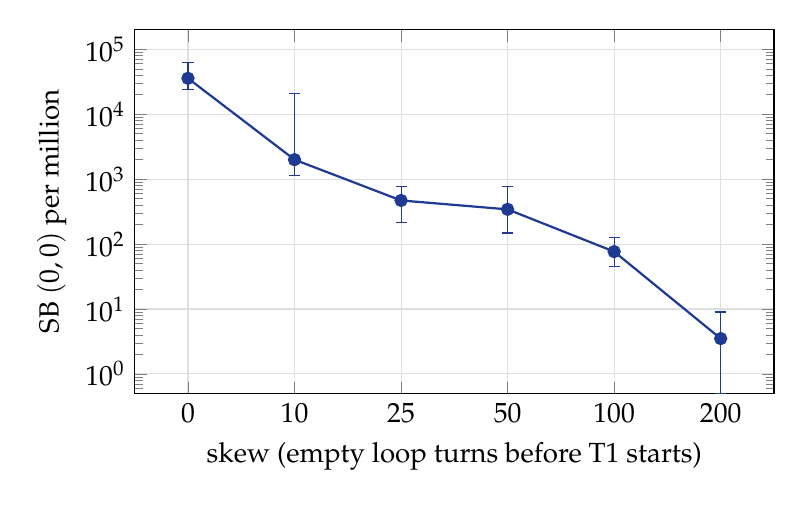
\begin{tikzpicture}
\begin{axis}[width=0.8\textwidth, height=6.2cm, ymode=log, ymin=0.5, ymax=2e5,
  xlabel={skew (empty loop turns before T1 starts)}, ylabel={SB \outc{0}{0} per million},
  symbolic x coords={0,10,25,50,100,200}, xtick=data, grid=major, grid style={gray!25},
  every axis plot/.append style={thick}]
\addplot[edgepo, mark=*, error bars/.cd, y dir=both, y explicit]
  coordinates {
  (0,35783.5) += (0,25938.5) -= (0,11855.5)
  (10,1997.5) += (0,19190.5) -= (0,866.5)
  (25,469.5) += (0,294.5) -= (0,255.5)
  (50,342.5) += (0,438.5) -= (0,194.5)
  (100,76.5) += (0,48.5) -= (0,31.5)
  (200,3.5) += (0,5.5) -= (0,3.0)
  };
\end{axis}
\end{tikzpicture}
\caption{SB \outc{0}{0} per million iterations as T1 is delayed. Points are the median of ten runs and the bars run from the minimum to the maximum. The axis is logarithmic. At skew 200 the minimum was 0, which a logarithmic axis cannot show, so that bar is cut at the bottom of the axis.}
\label{fig:skew}
\end{figure}

\begin{table}[!htbp]
\centering\small
\caption{SB \outc{0}{0} counts per run of one million iterations, for each skew. Ten runs each.}
\label{tab:skew}
\begin{tabular}{@{}rrrrrrr@{}}
\toprule
Skew & Median & Min & Max & Mean & Std.\ dev. & Total in $10^7$\\
\midrule
0 & 35{,}784 & 23{,}928 & 61{,}722 & 38{,}131 & 10{,}070 & 381{,}311\\
10 & 1{,}998 & 1{,}131 & 21{,}188 & 5{,}071 & 6{,}652 & 50{,}709\\
25 & 470 & 214 & 764 & 439 & 168 & 4{,}389\\
50 & 343 & 148 & 781 & 392 & 224 & 3{,}919\\
100 & 77 & 45 & 125 & 79 & 22 & 785\\
200 & 4 & 0 & 9 & 4 & 3 & 43\\
\bottomrule
\end{tabular}
\end{table}

The spread between runs is large, especially at skew 10, where one run gave more than ten times the median. Other work on the machine, the scheduling of the virtual CPUs and the exact cache state at the start of a run all change how often the two threads line up. This is why we report the median with the minimum and maximum, as \cref{sec:stats} explained. We also ran SB+mfence and MP at skews of 25 and 50, and both stayed at zero in all ten million iterations (\cref{app:data}).

\section{What the machine cannot show}

An x86-64 processor is TSO, so it never shows MP \outc{1}{0}, and our zero count is exactly what TSO predicts. It cannot show \gls{pso} at all, and we do not claim that it confirms PSO. Our experiment also cannot show SC, because no mainstream processor offers SC, which is the subject of \cref{ch:cost}.

\section{How our approach developed}
\label{sec:q2history}

Our first idea was simple: run the SB test on a real machine many times and look for the outcome $(0,0)$ that SC forbids. A first program of this kind can give a wrong answer for reasons that have nothing to do with the store buffer, so most of the work went into making the test measure the hardware.

The compiler was the first thing to deal with, since it may swap a store and a load before the hardware sees them. We fixed this with relaxed atomics and then read the machine code to confirm the order (\cref{sec:asm}). The second was the placement of the threads and the data: the two threads are pinned to different cores, and each variable has its own cache line, so that the coherence protocol does not decide the result.

The results then changed the plan. The count of $(0,0)$ depends strongly on how closely the two threads start together, so we made the skew a parameter and measured it (\cref{sec:skew}). This turned a side detail into an extra result of the experiment.

\section{Answer to Q2}
\label{sec:q2}

\begin{resultbox}{Answer to Q2: the store buffer is visible, and a fence hides it again}
On an x86-64 machine, SB \outc{0}{0}, which SC forbids, appeared 381{,}311 times in ten million tries. With \code{mfence} in both threads it never appeared, and the MP outcome that TSO forbids never appeared either. The theory predicts this, the checker agrees, the machine shows it, and the fence fixes it.
\end{resultbox}

% =====================================================================
\chapter{What Strong Ordering Costs, and Why SC Is Still Not Shipped (Q3)}
\label{ch:cost}
% =====================================================================

Q3 asks what strong ordering costs and why processors still do not offer sequential consistency. We answer it in two steps. First we measure what the \gls{sb} saves, using a small cost model. Then we ask whether that cost can be avoided in another way, and why \gls{sc} is still not shipped. All the numbers in this chapter come from our model, not from a real processor.

\section{The cost of waiting for every store}
\label{sec:boe}

Take a core with no store buffer, so it waits for every store to finish. This is the simplest way to build an SC machine. Suppose a fraction $f$ of the instructions are stores, each store takes $L$ cycles, and every other instruction takes one cycle. In 100 instructions, issuing takes 100 cycles and each of the $100f$ stores adds $L$ more. The average number of cycles per instruction (CPI) is therefore
\[
\text{CPI}_{\text{stall}} \approx 1 + f \cdot L.
\]
\Cref{tab:boe} evaluates this for a few values. With one store in ten instructions and a store that takes 100 cycles, the core runs at 11 cycles per instruction, eleven times slower than it could. These values only illustrate the formula.

\begin{table}[!htbp]
\centering\small
\caption{CPI of a core that waits for every store, from $1 + f\cdot L$. Illustrative values, computed by \texttt{cpi\_model.py}.}
\label{tab:boe}
\begin{tabular}{@{}lrrr@{}}
\toprule
Fraction of stores $f$ & $L = 4$ (cache hit) & $L = 100$ & $L = 300$ (main memory)\\
\midrule
0.05 & 1.20 & 6.00 & 16.00\\
0.10 & 1.40 & 11.00 & 31.00\\
0.20 & 1.80 & 21.00 & 61.00\\
\bottomrule
\end{tabular}
\end{table}

This gap is the reason store buffers exist, and so the reason \gls{tso} exists.

\section{When the buffer fills up}
\label{sec:buffervsfull}

With a buffer of $B$ entries, the core puts each store in the buffer and moves on. Memory takes the stores one at a time, oldest first, so the buffer is a FIFO queue. The core waits only when the buffer is full: it has nowhere to put the next store, so it stalls until the oldest store finishes and frees an entry. A buffer therefore moves the waiting later, and removes it only when the buffer never fills.

A slow store is what usually fills it. Memory finishes stores in order, so while one store that missed the cache takes 100 cycles, every store behind it waits too, while the core keeps issuing one instruction per cycle. If one instruction in ten is a store, about ten more stores join the queue during those 100 cycles. A buffer with fewer than about ten entries will often fill behind a single miss. A real buffer has a fixed number of entries, so we cannot make it as large as we like.

\section{A cycle-by-cycle cost model}
\label{sec:cpimodel}

The formula treats every store as equally slow and says nothing about the size of the buffer. To study this we wrote \code{cpi\_model.py} (\cref{app:code}), which counts the cycles of a simple core one at a time, with and without a buffer.

We use a model and not a measurement because on our laptops we cannot switch the store buffer off or change its size, and a real core hides memory delays in many other ways, so we could not tell which effect we were seeing. The cycles in the program are simulated processor cycles kept in a counter. They have nothing to do with the time the Python program takes, which is under a second.

\paragraph{The parameters.} \Cref{tab:cpiparams} lists what the model uses.

\begin{table}[!htbp]
\centering\small
\caption{The parameters of the cost model.}
\label{tab:cpiparams}
\begin{tabularx}{\textwidth}{@{}llX@{}}
\toprule
Symbol & Value & Meaning\\
\midrule
$N$ & 200{,}000 & number of instructions in one simulated run\\
$f$ & 0.10 & fraction of instructions that are stores\\
$m$ & 0.05 & fraction of stores that miss the cache\\
$L_{\text{hit}}$ & 4 cycles & time for a store whose line is in the cache\\
$L_{\text{miss}}$ & 100 cycles & time for a store whose line is not in the cache\\
$B$ & 1, 2, 4, 8, 16, 32, 56 & number of entries in the store buffer\\
\bottomrule
\end{tabularx}
\end{table}

The average store takes
\[
\bar{L} = (1 - m)\,L_{\text{hit}} + m\,L_{\text{miss}} = 0.95 \times 4 + 0.05 \times 100 = 8.8 \text{ cycles.}
\]
We compare two designs. The \emph{stall} design is the strict SC machine, where the core waits for every store. The \emph{buffer} design is the TSO-style machine.

\paragraph{How the program works.} A counter, \code{cycle}, holds the current cycle, and the program runs through the $N$ instructions one by one.
\begin{itemize}
\item Every instruction first adds one to \code{cycle}.
\item A random number below $f$ makes the instruction a store. For a store, a second random number below $m$ makes it a miss, which takes $L_{\text{miss}}$ cycles, and otherwise it is a hit and takes $L_{\text{hit}}$ cycles.
\item The buffer is a list of finish times, one for each store still waiting. At the start of every instruction the program removes the stores whose finish time has passed.
\item Memory handles one store at a time, so a store starts at the later of the current cycle and the time memory becomes free, and finishes after its latency. This makes the buffer a FIFO queue.
\item If there is room, the store is added and the core moves on. If all $B$ entries are in use, the core stalls: \code{cycle} jumps to the finish time of the oldest store, which is when an entry becomes free.
\item At the end, the CPI is \code{cycle} divided by $N$.
\end{itemize}

The buffer design is these few lines.

\begin{figure}[!htbp]
\centering
\begin{lstlisting}[style=vspython]
for _ in range(N):
    cycle += 1
    buffer = [t for t in buffer if t > cycle]     # remove completed stores
    if rng.random() < f:
        if len(buffer) == B:                      # wait for the oldest store
            cycle = buffer[0]
            buffer.pop(0)
        lat = l_miss if rng.random() < m else l_hit
        start = max(cycle, busy_until)            # FIFO order
        busy_until = start + lat
        buffer.append(busy_until)
return cycle / N
\end{lstlisting}
\caption{The main loop of the buffer design in \code{cpi\_model.py}.}
\label{fig:cpiloop}
\end{figure}

The stall design adds one cycle for every instruction and the full latency for every store. Both designs start from the same random seed and draw their random numbers in the same order, so they see the same stores and the same misses.

\section{Results}
\label{sec:cpiresults}

The stall design ran at a CPI of 1.873, which matches the formula, $1 + 0.10 \times 8.8 = 1.88$, up to the small difference of a random run. \Cref{fig:cpi} and \cref{tab:cpi} show the buffer design as the buffer grows.

\begin{figure}[!htbp]
\centering
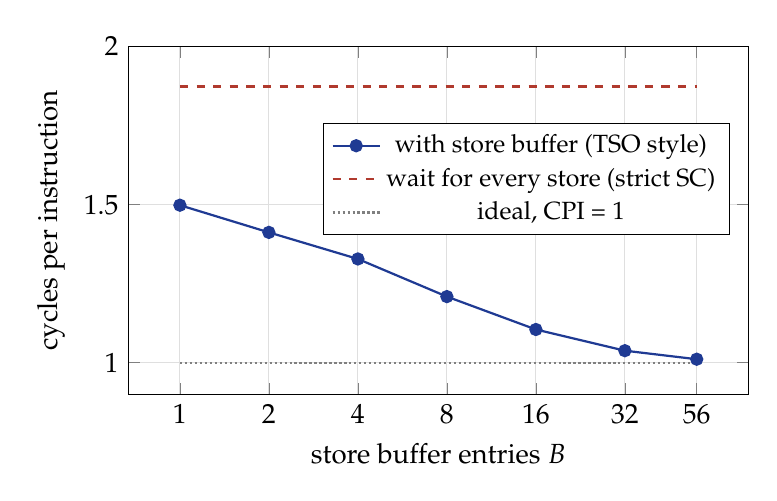
\begin{tikzpicture}
\begin{axis}[width=0.78\textwidth, height=6cm, xmode=log, log basis x=2,
  xlabel={store buffer entries $B$}, ylabel={cycles per instruction},
  xtick={1,2,4,8,16,32,56}, xticklabels={1,2,4,8,16,32,56},
  ymin=0.9, ymax=2.0, grid=major, grid style={gray!25}, legend style={font=\small, at={(0.97,0.78)}, anchor=north east}]
\addplot[edgepo, mark=*, thick] coordinates {(1,1.498) (2,1.412) (4,1.328) (8,1.209) (16,1.105) (32,1.038) (56,1.011)};
\addlegendentry{with store buffer (TSO style)}
\addplot[edgefr, dashed, thick, domain=1:56, samples=2] {1.873};
\addlegendentry{wait for every store (strict SC)}
\addplot[gray, densely dotted, thick, domain=1:56, samples=2] {1.0};
\addlegendentry{ideal, CPI = 1}
\end{axis}
\end{tikzpicture}
\caption{CPI from our cost model as the store buffer grows ($f = 0.10$, 5\% of stores miss, 4 and 100 cycles). The dashed line is the design that waits for every store. These are simulated cycles of a model, not measurements of a real processor.}
\label{fig:cpi}
\end{figure}

\begin{table}[!htbp]
\centering\small
\caption{CPI of the buffered design from the cost model. The design that waits for every store gives 1.873.}
\label{tab:cpi}
\begin{tabular}{@{}lrrrrrrr@{}}
\toprule
Entries $B$ & 1 & 2 & 4 & 8 & 16 & 32 & 56\\
\midrule
CPI & 1.498 & 1.412 & 1.328 & 1.209 & 1.105 & 1.038 & 1.011\\
\bottomrule
\end{tabular}
\end{table}

The ideal CPI is 1, so the stall design wastes 0.873 cycles on every instruction. A single entry removes about 43\% of this waste. With 8 entries only 0.209 is left, about a quarter, and with 56 entries only 0.011, so the core runs within about 1\% of the ideal.

The CPI falls as the buffer grows because a larger buffer can hold more stores while a slow one finishes. Behind one miss about ten stores arrive (\cref{sec:buffervsfull}). A buffer of 8 entries often fills before the miss completes and the core stalls, while a buffer of 56 entries takes the whole burst. The gain from each extra entry also shrinks. Doubling the buffer saves about 0.1 at first, but going from 16 to 32 entries saves only 0.067, and from 32 to 56 only 0.027. Once the buffer absorbs almost every burst, the core hardly ever stalls and there is little left to save.

\paragraph{When stores arrive faster than memory can finish them.} In the second experiment we raise the store fraction to $f = 0.20$ and the miss rate to $m = 0.10$. The average store now takes $0.9 \times 4 + 0.1 \times 100 = 13.6$ cycles, so every instruction brings $0.20 \times 13.6 = 2.72$ cycles of store work, and memory can do only one cycle of work per cycle. \Cref{tab:cpi2} shows the result.

\begin{table}[!htbp]
\centering\small
\caption{The second experiment: $f = 0.20$, $m = 0.10$, and the same latencies of 4 and 100 cycles.}
\label{tab:cpi2}
\begin{tabular}{@{}lr@{}}
\toprule
Design & CPI\\
\midrule
Wait for every store & 3.701\\
Buffer, $B = 8$ & 2.727\\
Buffer, $B = 56$ & 2.696\\
\bottomrule
\end{tabular}
\end{table}

The buffer still helps, bringing the CPI from 3.701 down to about 2.7, but now the buffer size hardly matters. The CPI sits at about 2.72, the amount of store work per instruction. The value 2.696 is slightly lower only because the program stops counting when the last instruction is issued, without waiting for the stores still in the buffer.

\section{What a store buffer can and cannot do}
\label{sec:bufferlimits}

A store buffer hides the delay of memory, and it does not make memory faster. Memory still finishes one store at a time, and each store takes the same number of cycles. The buffer only lets the core do other work in the meantime. When stores arrive slowly enough for memory to keep up, which is the common case, the buffer hides almost all of the delay. When they arrive faster, the buffer stays full and a larger one cannot help.

The FIFO buffer of the model is the one that makes a machine TSO: a store waits in the buffer while later loads go ahead, so the write-then-read order is the one that gets dropped. This gap is the reason TSO exists. The results show the size of the effect and why it happens, but they are not the performance of a real processor.

The next question is whether a machine can avoid this cost and still give SC. We look at one such idea, speculation, and then at why processors do not offer SC even so.

\section{Speculation}
\label{sec:spec}

The model says that a core that waits for every store pays a large price. Modern cores have a way to avoid waiting without giving up SC: they can guess, check, and undo. The second book describes the hardware for this, load speculation in \S5.1 and replay in \S5.2, built on the checkpoints of \S4.4.4\cite{sarangiNextGen}. Applied to memory ordering, the idea works as follows (\cref{fig:spec}).
\begin{itemize}
\item Let a load run early, before the earlier stores of the same thread have drained, and remember the address it read.
\item If another core writes that address before the load retires, the core learns of it through the coherence invalidation of \cref{sec:coherence}. The guess was wrong, because another core could now see the reordering. The core \emph{squashes}\index{squash} the load and everything after it, and runs them again.
\item If nobody touches that address, the guess was right and nothing is lost.
\end{itemize}

\begin{figure}[!htbp]
\centering
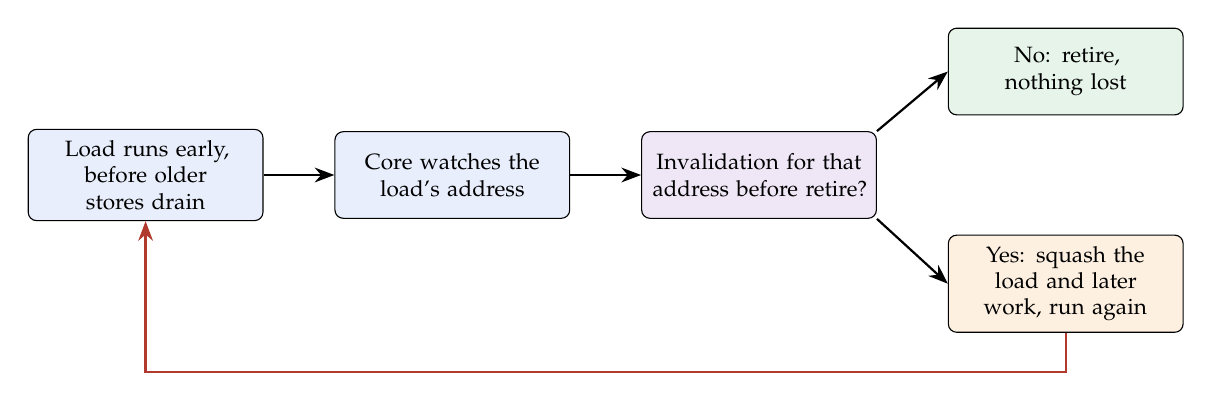
\begin{tikzpicture}[node distance=0.7cm and 0.9cm, s/.style={blk, text width=2.7cm, font=\footnotesize, minimum height=1.1cm}]
\node[s] (g) {Load runs early, before older stores drain};
\node[s, right=of g] (w) {Core watches the load's address};
\node[s, fill=boxpurple, right=of w] (q) {Invalidation for that address before retire?};
\node[s, fill=boxgreen, above right=0.2cm and 0.9cm of q] (ok) {No: retire, nothing lost};
\node[s, fill=boxorange, below right=0.2cm and 0.9cm of q] (sq) {Yes: squash the load and later work, run again};
\draw[arr] (g) -- (w); \draw[arr] (w) -- (q);
\draw[arr] (q.north east) -- (ok.west); \draw[arr] (q.south east) -- (sq.west);
\draw[arr, edgefr] (sq.south) -- ++(0,-0.5) -| (g.south);
\end{tikzpicture}
\caption{Guess, check and undo. The common case is the top branch, so the core runs at nearly the speed of a relaxed design while looking sequentially consistent from outside.}
\label{fig:spec}
\end{figure}

With this, a core can look sequentially consistent from outside and still run at nearly TSO speed in the common case, when threads share little. The price is extra hardware. The core must keep every speculative load and all the work after it in an undoable state until the older stores have drained, and it must watch each of those addresses. This paper describes the idea in words and leaves a simulation of it to future work.

\section{Four reasons SC is still not demanded}
\label{sec:fourreasons}

Even if speculation makes SC nearly as fast as TSO, no mainstream processor offers it. We weighed four explanations (\cref{tab:reasons}).

\begin{table}[!htbp]
\centering\small
\caption{Four candidate reasons why processors do not offer SC, and the evidence in this paper for each.}
\label{tab:reasons}
\begin{tabularx}{\textwidth}{@{}lXX@{}}
\toprule
Reason & What it says & What our work shows\\
\midrule
1. Habit and compatibility & Existing software and instruction sets already assume TSO or weaker, so a stronger model buys little for old code. & x86 has been TSO for a long time\cite{owens2009}.\\
2. Hardware cost & Speculation needs tracking bits, checkpoints and a way to roll back, and these cost chip area and design effort. & \Cref{sec:spec}: every early load and the work after it must stay undoable until older stores drain.\\
3. Software already copes & Data-race-free programs see SC anyway (DRF-SC), and the few places that need order use fences. & \Cref{par:drf}: the fences are already inside locks and atomics.\\
4. Risk under sharing & When threads share a lot, guesses fail often, and frequent squashes waste work. & \Cref{fig:spec}: the bottom branch is the expensive one, and heavy sharing makes it common.\\
\bottomrule
\end{tabularx}
\end{table}

\paragraph{What DRF-SC says.}\label{par:drf}\index{DRF-SC}\index{data race} Most programmers never write a \gls{fence}. They use locks and atomic variables, and their programs still behave as if the machine were SC. The reason is a simple rule. A \emph{data race} happens when two threads use the same variable at the same time, at least one of them writes, and no lock or atomic operation orders the two accesses. The rule, called \emph{\gls{drfsc}}, says that a program with no data races behaves as if the machine were SC, whatever the hardware does underneath. The fences are already inside the lock and atomic operations, put there by the people who wrote the libraries and the compilers. Our \gls{litmus}s SB and MP have data races on purpose, which is why they can show results that SC forbids. If we protected \code{x} and \code{y} with a lock, we would never see \outc{0}{0}.

\paragraph{Which reason we find most convincing.} We find reason 3 the most convincing, with reason 1 as its partner. The SB outcome is real, as \cref{ch:hw} showed, but it reaches a programmer only when the program has a data race. Programs that use locks and atomics properly already get SC behaviour through the DRF-SC contract, and the cost of that contract on x86 is small and paid only at the few places that need it. On x86 only a write followed by a read can be reordered, so only the strongest atomic store needs an extra instruction, and every other access is an ordinary move. Since software already gets SC where it asks for it, there is little demand for hardware that gives SC everywhere. Reason 1 then explains why the situation does not change: the software that exists was written for TSO or weaker, so a stronger hardware model would help little of it. Reasons 2 and 4 are real costs, but they would matter only if there were demand to pay them.

\section{Why go weaker than TSO at all?}
\label{sec:weaker}

The same logic that produced the store buffer keeps going. Each arrow a model drops gives the hardware a new freedom. \gls{pso} drops \WW\ so that a store that hits the cache need not wait behind one that misses (\cref{sec:pso}). More freedom means more chances to overlap slow memory work with useful work. The price is paid by the programmer, who must now write fences, such as the store-store fence that MP needed under PSO in \cref{fig:mpfence}, or use locks and atomics so that DRF-SC places the fences for them. Choosing a point on the ladder is a trade between speed and how easy the machine is to reason about.

\section{How our approach developed}
\label{sec:q3history}

We started from the simple formula $1 + f\cdot L$ of \cref{sec:boe}, which shows that waiting for every store is slow. It has two gaps. It says nothing about the size of the buffer, and it treats every store as equally slow.

Studying the buffer size was the first difficulty. We could not change the store buffer of our own laptops, and a real core hides memory delays in other ways too, so a measurement would not isolate the effect. We therefore wrote the cycle-by-cycle model of \cref{sec:cpimodel}.

A claim in our first draft of this chapter was also wrong: that one buffer entry removes more than half of the waiting. When we checked it against the model output, the true figure was about 43\%, so we corrected the text.

A second experiment then changed the picture. The first run suggested that a bigger buffer always helps, which is true only while stores arrive more slowly than memory can finish them. Raising the store and miss rates showed the other case, where the buffer size hardly matters (\cref{tab:cpi2}).

\section{Answer to Q3}
\label{sec:q3}

\begin{resultbox}{Answer to Q3: strong ordering is costly without tricks, and the remaining reasons are about software}
A core that waits for every store pays a large price: in our model, CPI 1.873 against 1.011 for the same core with a 56-entry store buffer. That gap is why store buffers, and therefore TSO, exist. Speculation can, in principle, give SC behaviour at nearly TSO speed, at the cost of extra hardware and of wasted work when threads share heavily. We think the main reason processors still do not offer SC is that software does not need it: data-race-free programs already see SC through the DRF-SC contract, fences are needed at only a few places, and existing software was written for TSO or weaker models.
\end{resultbox}

% =====================================================================
\chapter{Conclusion and Future Work}
\label{ch:conclusion}
% =====================================================================

\section{What the paper shows}

We began with a two-thread program whose result looks impossible and asked what the smallest hardware feature is that makes it possible. We found that a \gls{sb} is enough on its own.

\begin{itemize}
\item \textbf{A store buffer is the smallest hardware feature that breaks SC.} SB \outc{0}{0} is the witness. The cycle argument explains it: the store buffer removes the write-then-read arrows, and the cycle in the SB graph disappears (\cref{sec:sbgraph}).
\item \textbf{The models form a strict ladder (Q1).} \gls{sc} sits inside \gls{tso}, which sits inside \gls{pso}. Removing arrows cannot create a cycle, the checker confirms the chain on 2005 programs, SB separates SC from TSO and MP separates TSO from PSO (\cref{sec:mpgraph}). An independent simulation of the store buffers agrees with the checker on every program we tried.
\item \textbf{The machine shows it (Q2).} On an x86-64 machine, SB \outc{0}{0} appeared in a few percent of the tries, while MP \outc{1}{0}, which TSO forbids, never appeared.
\item \textbf{A fence puts the dropped arrows back.} With \code{mfence} in both threads the SB outcome disappeared on the machine, and the checker shows the cycle returning.
\item \textbf{The store buffer exists because waiting for stores is expensive, and SC is not shipped because software does not ask for it (Q3).} In our model a large buffer removes almost all the waiting. Speculation could give SC at nearly that speed, but data-race-free programs already see SC through \gls{drfsc}, and existing software assumes TSO or weaker.
\end{itemize}

\section{Limits of this work}

\begin{itemize}
\item Only TSO was observed on hardware. PSO appears through the checker and the simulation only, as a teaching model.
\item We studied two \gls{litmus}s and their fenced versions. They are enough for our questions, and many more exist.
\item Our hardware runs used a cloud virtual machine with two virtual CPUs. The ordering rules are those of the Intel processor underneath, but the counts, especially their spread, depend on the machine and its load.
\item A zero count is not a proof. Only the checker proves that an outcome is impossible; the hardware runs bound how rare it is.
\item The cost numbers of \cref{ch:cost} come from a simple model, not from measurements of a real processor, and the argument about speculation is reasoned, not simulated.
\end{itemize}

\section{Future work}

The natural next steps are the ones we left out on purpose to keep the paper at the level of the course. They are more litmus tests, such as tests with three or four threads; processors with weaker models, such as ARM, where MP \outc{1}{0} can be observed; measuring the cost of fences and of sequentially consistent atomics on real hardware; and a simulation of a speculative core that offers SC, to put numbers on the argument of \cref{sec:spec}.

% =====================================================================
\appendix
\chapter{Plagiarism Report}
\label{app:plag}
% =====================================================================

The Turnitin similarity report for this paper is placed here. It is generated from the same file that is submitted on Gradescope.

\chapter{Readability Indices}
\label{app:read}

\Cref{tab:read} gives the readability indices of the entire text of this paper, as reported by the page \url{https://www.analyzemywriting.com/readability_indices.html}. Each value is the grade level, the number of years of schooling a reader needs to follow the text easily. The script \code{readability.py} (\cref{app:code}) is also included with the code and measures the prose of the main chapters in the same way, but the values required by the course are the ones in the table.

\begin{table}[h]
\centering\small
\caption{Readability indices of the entire text of the paper.}
\label{tab:read}
\begin{tabular}{@{}lr@{}}
\toprule
Readability score (index) & Grade level of entire text\\
\midrule
Gunning fog & 10.23\\
Flesch--Kincaid & 7.75\\
SMOG & 9.37\\
Coleman--Liau & 8.38\\
Automated readability & 8.87\\
\midrule
Average grade level & 8.92\\
Median grade level & 8.87\\
\bottomrule
\end{tabular}
\end{table}

The five grade levels lie between about 7.7 and 10.2, which is the band of general adult reading, and their average is 8.92.

% =====================================================================
\chapter{Weekly Schedule of the Work}
\label{app:schedule}
% =====================================================================

\Cref{tab:schedule} lists the work done on this paper in each week from 30 August to 16 November. One week had no project work, and chapters were written while the experiments were still running.

The Gantt chart in \cref{fig:gantt} shows the same schedule as bars.

\begin{figure}[!htbp]
\centering
\begin{ganttchart}[
  hgrid, vgrid={*{11}{draw=black!20}},
  x unit=0.85cm, y unit title=0.6cm, y unit chart=0.55cm,
  title height=1, bar height=0.6,
  title/.append style={draw=black!40, fill=boxgrey},
  bar/.append style={draw=black!70, thick},
  bar label font=\footnotesize, title label font=\footnotesize,
  include title in canvas=false]{1}{11}
\gantttitle{Week}{11} \\
\gantttitlelist{1,...,11}{1} \\
\ganttbar[bar/.append style={fill=boxgrey}]{Topic, questions, scope}{1}{1} \\
\ganttbar[bar/.append style={fill=boxgrey}]{Reading and notes}{2}{2} \\
\ganttbar[bar/.append style={fill=boxblue}]{Background chapters}{2}{2} \ganttbar[bar/.append style={fill=boxblue}]{}{4}{4} \\
\ganttbar[bar/.append style={fill=boxblue}]{Rules chapter (math)}{4}{5} \\
\ganttbar[bar/.append style={fill=boxgreen}]{Q1: checker, tests, simulation}{5}{7} \\
\ganttbar[bar/.append style={fill=boxgreen}]{Q1 chapter}{6}{7} \\
\ganttbar[bar/.append style={fill=boxorange}]{Q2: C test and real runs}{6}{7} \\
\ganttbar[bar/.append style={fill=boxorange}]{Q2 chapter}{8}{8} \\
\ganttbar[bar/.append style={fill=boxpurple}]{Q3: cost model, experiments}{8}{9} \\
\ganttbar[bar/.append style={fill=boxpurple}]{Q3 chapter}{9}{9} \\
\ganttbar[bar/.append style={fill=boxgrey}]{Introduction and conclusion}{8}{9} \\
\ganttbar[bar/.append style={fill=boxgrey}]{Full draft and advisor/TA review}{9}{9} \\
\ganttbar[bar/.append style={fill=boxgrey}]{Number check, feedback, formatting}{10}{10} \\
\ganttbar[bar/.append style={fill=boxgrey}]{Appendices, Turnitin, final build, upload}{11}{11}
\end{ganttchart}
\caption{Gantt chart of the work, drawn from \cref{tab:schedule}. Weeks run from 30 August (week 1) to 16 November (week 11). Week 3 had no project work. Blue marks the theory, green Q1, orange Q2, purple Q3 and grey the rest of the paper.}
\label{fig:gantt}
\end{figure}

\begin{longtable}{@{}>{\raggedright}p{0.9cm}>{\raggedright}p{2.5cm}>{\raggedright}p{7.2cm}>{\raggedright\arraybackslash}p{4.2cm}@{}}
\caption{The week-by-week schedule of the work.}\label{tab:schedule}\\
\toprule
Week & Dates & What was done & Output at the end of the week\\
\midrule
\endfirsthead
\toprule
Week & Dates & What was done & Output at the end of the week\\
\midrule
\endhead
\bottomrule
\endlastfoot
1 & 30 Aug -- 5 Sep & Chose the topic. Read the basics from the course book. Wrote down the 3 questions and fixed the scope (SC, TSO, PSO only). & One page: topic, 3 questions, scope \\
2 & 6 -- 12 Sep & Read the main papers and took notes in plain words. Agreed on one notation (po, rf, co, fr). Started the hardware background: memory, store buffer, two cores. & Notes, shared .bib file, rough background \\
3 & 13 -- 19 Sep & No project work. & None \\
4 & 20 -- 26 Sep & Finished the background chapters. Worked out SB and MP by hand and started writing the rules of each model as math (program order, graphs, cycles). & Background chapters, half of the rules chapter \\
5 & 27 Sep -- 3 Oct & Finished the rules chapter and checked it by hand on the litmus tests. Q1: wrote the first version of the checker and ran the 5 hand-written tests. Found that TSO and PSO needed a second graph and changed the rules. & Rules chapter, checker passing the hand-written tests \\
6 & 4 -- 10 Oct & Q1: added the random programs, wrote the separate store-buffer simulation and compared it with the checker. Began writing the Q1 chapter. Started the C litmus test for Q2. & Counts for Q1, first draft of the Q1 chapter, first Q2 code \\
7 & 11 -- 17 Oct & Q1: tidied the code into one file per model and finished the Q1 chapter. Q2: ran the test on a real machine, then repeated it with fences and different offsets. & Q1 chapter, raw data for Q2 \\
8 & 18 -- 24 Oct & Q2: wrote the chapter from the raw data and summary table. Q3: wrote the first version of the cost model. Drafted the introduction. & Q2 chapter, first cost model \\
9 & 25 -- 31 Oct & Q3: ran the buffer-size experiments, corrected the model text and wrote the Q3 chapter. Drafted the conclusion. Joined everything into one full draft and showed it to the advisor and a TA. & Q3 chapter, full draft v1 \\
10 & 1 -- 8 Nov & Checked every number in the text against the program output. Fixed the feedback on the draft. Applied the course formatting rules (A4, 12 pt, copyright page, acknowledgement, lists, index, glossary, code as listings, diagrams as TikZ). & Draft that follows most formatting rules \\
11 & 9 -- 16 Nov & Moved long explanations to appendices. Ran the readability and Turnitin checks. Final build and read-through. Uploaded on Gradescope with all authors added. & Submitted paper \\
\end{longtable}

\chapter{Source Code}
\label{app:code}

Every program used in this paper is printed below in full. The same files, with their raw outputs, are in the repository listed in \cref{app:repro}.

\section{The arrow helpers: \texttt{graph.py}}
The small functions that build each kind of arrow (\cref{sec:graphfile}).

\begin{lstlisting}[style=vspython]
"""Helpers for building order graphs."""

# Pairs restored by each fence
FENCE_RESTORES = {
    "mfence": {"RR", "RW", "WW", "WR"},
    "stbar": {"WW"},
}


def pair(a, b):
    return a.kind + b.kind


def program_order(events):
    pairs = []
    for a in events:
        for b in events:
            if a.thread is None or b.thread is None:
                continue  # initial writes have no thread
            if a.thread == b.thread and a.index < b.index:
                pairs.append((a, b))

    return pairs


def preserved_program_order(events, kept):
    arrows = []
    for a, b in program_order(events):
        if a.var != b.var:
            if pair(a, b) in kept:
                arrows.append((a, b))
        elif pair(a, b) != "WR":  # W -> R may get its value from the store buffer
            arrows.append((a, b))

    return arrows


def fence_arrows(events, fences):
    arrows = []
    for a, b in program_order(events):
        for tid, pos, kind in fences:
            between = (a.thread == tid and a.index < pos < b.index)
            if between and pair(a, b) in FENCE_RESTORES[kind]:
                arrows.append((a, b))

    return arrows


def external_reads_from(reads_from):
    return [(write, read) for write, read in reads_from
            if write.thread != read.thread]


def from_read_arrows(reads_from, write_order):
    arrows = []
    for write, read in reads_from:
        for first, later in write_order:
            if first is write:
                arrows.append((read, later))  # read before later writes

    return arrows


def same_address_arrows(events, reads_from, write_order):
    # Same-address program order, reads-from, write order and from-read
    same_po = [(a, b) for a, b in program_order(events)
               if a.var == b.var]

    return (same_po + reads_from + write_order
            + from_read_arrows(reads_from, write_order))
\end{lstlisting}

\section{Model SC: \texttt{sc.py}}
One graph with every program-order arrow (\cref{sec:modeltable}).

\begin{lstlisting}[style=vspython]
"""SC keeps every program-order pair."""
from graph import program_order, from_read_arrows


def graphs(events, fences, reads_from, write_order):
    arrows = (program_order(events) + reads_from + write_order
              + from_read_arrows(reads_from, write_order))
    
    return [arrows]
\end{lstlisting}

\section{Model TSO: \texttt{tso.py}}
The global graph and the graph of one address. The file \texttt{pso.py} below differs only in the set of kept pairs.

\begin{lstlisting}[style=vspython]
"""TSO relaxes W -> R because of the store buffer."""
from graph import (preserved_program_order, fence_arrows, external_reads_from,
                   from_read_arrows, same_address_arrows)

KEPT = {"RR", "RW", "WW"}


def graphs(events, fences, reads_from, write_order):
    global_arrows = (preserved_program_order(events, KEPT)
                     + fence_arrows(events, fences)
                     + external_reads_from(reads_from)
                     + write_order
                     + from_read_arrows(reads_from, write_order))
    
    return [global_arrows, same_address_arrows(events, reads_from, write_order)]
\end{lstlisting}

\section{Model PSO: \texttt{pso.py}}
The same as \texttt{tso.py}, with one pair fewer kept.

\begin{lstlisting}[style=vspython]
"""PSO relaxes W -> R and W -> W."""
from graph import (preserved_program_order, fence_arrows, external_reads_from,
                   from_read_arrows, same_address_arrows)

KEPT = {"RR", "RW"}


def graphs(events, fences, reads_from, write_order):
    global_arrows = (preserved_program_order(events, KEPT)
                     + fence_arrows(events, fences)
                     + external_reads_from(reads_from)
                     + write_order
                     + from_read_arrows(reads_from, write_order))
    
    return [global_arrows, same_address_arrows(events, reads_from, write_order)]
\end{lstlisting}

\section{The test programs: \texttt{tests.py}}
The start of the file: the five litmus tests, their target outcomes and the expected answers. The 2000 random programs follow in the same file and are not printed here, but they are in the repository.

\begin{lstlisting}[style=vspython]
"""
tests.py -- every test program the checker uses.

A program is a list of threads. A thread is a list of instructions:
    ("W", var, value)    write value to var
    ("R", reg, var)      read var into register reg
    ("F", kind)          fence, kind is "mfence" or "stbar"
"""

# ---- the 5 hand-written litmus tests ---------------------------------
LITMUS = {
    "SB":         [[("W", "x", 1), ("R", "r0", "y")],
                   [("W", "y", 1), ("R", "r1", "x")]],
    "SB+mfences": [[("W", "x", 1), ("F", "mfence"), ("R", "r0", "y")],
                   [("W", "y", 1), ("F", "mfence"), ("R", "r1", "x")]],
    "MP":         [[("W", "x", 1), ("W", "y", 1)],
                   [("R", "r0", "y"), ("R", "r1", "x")]],
    "MP+stbar":   [[("W", "x", 1), ("F", "stbar"), ("W", "y", 1)],
                   [("R", "r0", "y"), ("R", "r1", "x")]],
    "OwnWrite":   [[("W", "x", 1), ("R", "r0", "x")]],
}

# The outcome each litmus test asks about.
TARGET = {
    "SB": {"r0": 0, "r1": 0},      "SB+mfences": {"r0": 0, "r1": 0},
    "MP": {"r0": 1, "r1": 0},      "MP+stbar":   {"r0": 1, "r1": 0},
    "OwnWrite": {"r0": 0},
}

# Expected answer for (SC, TSO, PSO): A = allowed, F = forbidden.
EXPECTED = {
    "SB": "FAA", "SB+mfences": "FFF", "MP": "FFA",
    "MP+stbar": "FFF", "OwnWrite": "FFF",
}

# ---- 2000 random programs (seed 305, made once and saved here) --------
RANDOM_TESTS = [
    ...   # 2000 programs, saved so every run uses the same ones
]
\end{lstlisting}

\section{The checker: \texttt{checker.py}}
The checker of \cref{ch:checker}. It does the checking only; the arrows come from the model files. It has no outside dependencies.

\begin{lstlisting}[style=vspython]
from itertools import permutations, product

from tests import LITMUS, TARGET, EXPECTED, RANDOM_TESTS
import sc
import tso
import pso


MODELS = [("SC", sc), ("TSO", tso), ("PSO", pso)]


class Event:
    def __init__(self, kind, var, value=None, reg=None,
                 thread=None, index=None, label=None):
        self.kind = kind
        self.var = var
        self.value = value
        self.reg = reg
        self.thread = thread
        self.index = index
        self.label = label

    def __repr__(self):
        return self.label


def find_variables(test):
    var_list = set()

    for thread in test:
        for op in thread:
            if op[0] == "W":
                var_list.add(op[1])
            elif op[0] == "R":
                var_list.add(op[2])

    return sorted(var_list)


def make_label(cnt):
    label = ""
    while cnt >= 0:
        label = chr(ord("a") + cnt % 26) + label
        cnt = cnt // 26 - 1
    return label


def make_events(test):
    var_list = find_variables(test)
    events = []
    fences = []

    # Add the initial write for every variable before the program events.
    for var in var_list:
        events.append(Event("W", var, value=0, label="init_" + var))

    cnt = 0
    for tid, thread in enumerate(test):
        for pos, op in enumerate(thread):
            if op[0] == "W":
                _, var, val = op
                events.append(Event("W", var, value=val,
                                    thread=tid, index=pos,
                                    label=make_label(cnt)))
                cnt += 1

            elif op[0] == "R":
                _, reg, var = op
                events.append(Event("R", var, reg=reg,
                                    thread=tid, index=pos,
                                    label=make_label(cnt)))
                cnt += 1

            else:
                _, kind = op
                fences.append((tid, pos, kind))

    return events, fences, var_list


def has_cycle(nodes, arrows):
    indeg = {}
    adj = {}

    for node in nodes:
        indeg[node] = 0
        adj[node] = []

    for u, v in set(arrows):
        adj[u].append(v)
        indeg[v] += 1

    st = []
    for node in nodes:
        if indeg[node] == 0:
            st.append(node)

    cnt = 0
    while st:
        u = st.pop()
        cnt += 1

        for v in adj[u]:
            indeg[v] -= 1
            if indeg[v] == 0:
                st.append(v)

    return cnt != len(nodes)


def all_guesses(events, var_list):
    reads = [e for e in events if e.kind == "R"]

    writes = {}
    for var in var_list:
        writes[var] = [e for e in events if e.kind == "W" and e.var == var]

    read_opts = []
    for r in reads:
        read_opts.append(writes[r.var])

    write_opts = []
    for var in var_list:
        init = writes[var][0]
        other = writes[var][1:]

        arr = []
        for p in permutations(other):
            arr.append([init] + list(p))

        write_opts.append(arr)

    guesses = []
    for chosen in product(*read_opts):
        reads_from = list(zip(chosen, reads))

        for orders in product(*write_opts):
            write_order = []
            for order in orders:
                for i in range(len(order)):
                    for j in range(i + 1, len(order)):
                        write_order.append((order[i], order[j]))

            guesses.append((reads_from, write_order, orders))

    return guesses


def guess_is_possible(events, fences, model, guess):
    reads_from, write_order, _ = guess

    for arrows in model.graphs(events, fences, reads_from, write_order):
        if has_cycle(events, arrows):
            return False

    return True


def outcome_of(guess):
    reads_from, _, orders = guess

    reg_val = []
    for write, read in reads_from:
        reg_val.append((read.reg, write.value))

    # Sorting makes equivalent register outcomes have the same set representation.
    reg_val = tuple(sorted(reg_val))

    memory = []
    for order in orders:
        last = order[-1]
        memory.append((last.var, last.value))

    # var_list is sorted, so the final memory values are already in a fixed order.
    return reg_val, tuple(memory)


def check(test, model):
    events, fences, var_list = make_events(test)
    allowed = set()

    for guess in all_guesses(events, var_list):
        if guess_is_possible(events, fences, model, guess):
            allowed.add(outcome_of(guess))

    return allowed


def outcome_is_allowed(allowed, target):
    for registers, _ in allowed:
        vals = dict(registers)
        ok = True

        for reg, val in target.items():
            if vals[reg] != val:
                ok = False
                break

        if ok:
            return True

    return False


def run_litmus_tests():
    ok = True
    print("test outcome SC TSO PSO as expected?")

    for name, test in LITMUS.items():
        verdict = ""

        for _, model in MODELS:
            allowed = check(test, model)
            if outcome_is_allowed(allowed, TARGET[name]):
                verdict += "A"
            else:
                verdict += "F"

        match = (verdict == EXPECTED[name])
        if not match:
            ok = False

        print(f"{name:<12s} {str(tuple(TARGET[name].values())):<12s} "
              f"{verdict[0]:>3s} {verdict[1]:>3s} {verdict[2]:>3s}   "
              f"{'yes' if match else 'NO'}")

    return ok


def run_subset_check():
    progs = list(LITMUS.values()) + RANDOM_TESTS

    fail = 0
    sc_less = 0
    tso_less = 0

    for test in progs:
        a = check(test, sc)
        b = check(test, tso)
        c = check(test, pso)

        if not (a <= b and b <= c):
            fail += 1

        if a < b:
            sc_less += 1

        if b < c:
            tso_less += 1

    print(f"\nSubset check on {len(progs)} programs")
    print("  SC <= TSO <= PSO fails:            ", fail)
    print("  SC allows strictly less than TSO:  ", sc_less)
    print("  TSO allows strictly less than PSO: ", tso_less)

    return fail == 0


def print_candidates(name):
    test = LITMUS[name]
    events, fences, var_list = make_events(test)

    print(f"\nCandidate executions of {name}")
    print(f"  {'who each read reads from':<34s} {'(r0,r1)':<8s} "
          f"{'SC':>7s} {'TSO':>7s} {'PSO':>7s}")

    for guess in all_guesses(events, var_list):
        reads_from = guess[0]

        reads = []
        for write, read in reads_from:
            reads.append(f"{read.label} reads {write.label}")

        registers, _ = outcome_of(guess)
        vals = "(" + ", ".join(str(v) for _, v in registers) + ")"

        ans = []
        for _, model in MODELS:
            if guess_is_possible(events, fences, model, guess):
                ans.append("allowed")
            else:
                ans.append("cycle")

        print(f"  {', '.join(reads):<34s} {vals:<8s} "
              f"{ans[0]:>7s} {ans[1]:>7s} {ans[2]:>7s}")


def main():
    litmus_ok = run_litmus_tests()

    print_candidates("SB")
    print_candidates("MP")

    subset_ok = run_subset_check()

    ok = litmus_ok and subset_ok
    print("\nAll checks passed:", "yes" if ok else "NO")

    return ok


if __name__ == "__main__":
    import sys
    sys.exit(0 if main() else 1)
\end{lstlisting}

\section{The store-buffer simulation: \texttt{sb\_machine.py}}
The step-by-step simulation of \cref{sec:sim}. It imports the checker and the tests.

\begin{lstlisting}[style=vspython]
"""Store-buffer simulation for SC, TSO and PSO.

Explores the possible instruction and buffer-drain steps, then compares the
final outcomes with checker.py.

SC   writes go straight to memory
TSO  only the oldest buffered store can drain
PSO  stores to different addresses may drain out of order

mfence waits for an empty buffer; stbar leaves a marker in the buffer.

Run: python3 sb_machine.py
"""
from checker import check, MODELS
from tests import LITMUS, RANDOM_TESTS

# Buffer entries: ("S", address, value) or an stbar marker ("B",)
# State: program counters, buffers, memory and register values
# Tuples let us store each state in a set.


def addresses_used(test):
    names = set()
    for thread in test:
        for instruction in thread:
            if instruction[0] == "W":
                names.add(instruction[1])
            elif instruction[0] == "R":
                names.add(instruction[2])
    return sorted(names)


def start_state(test):
    memory = []
    for address in addresses_used(test):
        memory.append((address, 0))         # every address starts at 0
    pcs = tuple(0 for _ in test)
    buffers = tuple(() for _ in test)       # empty buffers
    return (pcs, buffers, tuple(memory), ())


def write_to_memory(memory, address, value):
    """Copy memory and update one address."""
    as_dict = dict(memory)
    as_dict[address] = value
    return tuple(sorted(as_dict.items()))


def replace_item(items, index, new_item):
    """Copy a tuple with one item replaced."""
    return items[:index] + (new_item,) + items[index + 1:]


def may_drain(buffer, i, model):
    """Whether entry i can drain now."""
    entry = buffer[i]
    if entry[0] != "S":
        return False  # marker
    if model == "TSO":
        return i == 0  # FIFO
    # PSO: check older entries
    for older in buffer[:i]:
        if older[0] == "B":
            return False  # older stbar
        if older[1] == entry[1]:
            return False  # older store to the same address
    return True


def read_value(buffer, memory, address):
    """Read the newest matching store, or memory if there is none."""
    for entry in reversed(buffer):  # newest first
        if entry[0] == "S" and entry[1] == address:
            return entry[2]
    return dict(memory)[address]


def next_states(state, test, model):
    """Possible states after one step."""
    pcs, buffers, memory, regs = state
    result = []

    for t in range(len(test)):
        thread = test[t]
        buffer = buffers[t]

        # Thread t runs its next instruction
        if pcs[t] < len(thread):
            instruction = thread[pcs[t]]
            new_pcs = replace_item(pcs, t, pcs[t] + 1)

            if instruction[0] == "W":
                _, address, value = instruction
                if model == "SC":
                    # SC: straight to memory
                    new_memory = write_to_memory(memory, address, value)
                    result.append((new_pcs, buffers, new_memory, regs))
                else:
                    # add to its buffer
                    new_buffer = buffer + (("S", address, value),)
                    result.append((new_pcs, replace_item(buffers, t, new_buffer),
                                   memory, regs))

            elif instruction[0] == "R":
                _, register, address = instruction
                value = read_value(buffer, memory, address)
                new_regs = tuple(sorted(regs + ((register, value),)))
                result.append((new_pcs, buffers, memory, new_regs))

            else:                           # a fence
                _, kind = instruction
                if kind == "mfence":
                    # wait for an empty buffer
                    if len(buffer) == 0:
                        result.append((new_pcs, buffers, memory, regs))
                elif kind == "stbar":
                    if model == "PSO":
                        new_buffer = buffer + (("B",),)
                        result.append((new_pcs, replace_item(buffers, t, new_buffer),
                                       memory, regs))
                    else:
                        # SC and TSO already keep W -> W order
                        result.append((new_pcs, buffers, memory, regs))

        # Hardware drains an entry from buffer t
        if len(buffer) > 0 and buffer[0][0] == "B":
            # remove a marker at the front
            result.append((pcs, replace_item(buffers, t, buffer[1:]),
                           memory, regs))
        for i in range(len(buffer)):
            if may_drain(buffer, i, model):
                entry = buffer[i]
                new_buffer = buffer[:i] + buffer[i + 1:]
                new_memory = write_to_memory(memory, entry[1], entry[2])
                result.append((pcs, replace_item(buffers, t, new_buffer),
                               new_memory, regs))

    return result


def all_final_outcomes(test, model):
    """Explore step orders and collect final outcomes."""
    start = start_state(test)
    seen = {start}
    to_visit = [start]
    outcomes = set()

    while len(to_visit) > 0:
        state = to_visit.pop()
        pcs, buffers, memory, regs = state

        # All instructions done and buffers empty
        all_threads_done = all(pcs[t] == len(test[t]) for t in range(len(test)))
        all_buffers_empty = all(len(b) == 0 for b in buffers)
        if all_threads_done and all_buffers_empty:
            outcomes.add((regs, memory))

        for new_state in next_states(state, test, model):
            if new_state not in seen:
                seen.add(new_state)
                to_visit.append(new_state)

    return outcomes, len(seen)


def main():
    print("Store-buffer machine simulation, compared with checker.py")
    print("=" * 60)
    all_agree = True

    print("%-12s %-4s %8s %10s %10s  %s" % (
        "test", "model", "states", "machine", "checker", "same?"))
    for name, test in LITMUS.items():
        for model_name, model_file in MODELS:
            machine, state_count = all_final_outcomes(test, model_name)
            checker_result = check(test, model_file)
            same = (machine == checker_result)
            if not same:
                all_agree = False
            print("%-12s %-4s %8d %10d %10d  %s" % (
                name, model_name, state_count, len(machine),
                len(checker_result), "yes" if same else "NO"))

    differences = 0
    for test in RANDOM_TESTS:
        for model_name, model_file in MODELS:
            machine, _ = all_final_outcomes(test, model_name)
            if machine != check(test, model_file):
                differences += 1
    if differences > 0:
        all_agree = False
    print("\nRandom programs: %d, models per program: 3" % len(RANDOM_TESTS))
    print("  (program, model) pairs where machine and checker differ: %d"
          % differences)
    print("\nMachine and checker agree everywhere:", "yes" if all_agree else "NO")
    return all_agree


if __name__ == "__main__":
    import sys
    sys.exit(0 if main() else 1)
\end{lstlisting}

\section{The litmus harness: \texttt{litmus.c}}
The C program of \cref{ch:hw}.

\begin{lstlisting}[style=vsc]
/*
 * Run the SB and MP litmus tests on x86-64.
 *
 * Two threads run on separate cores. Each iteration starts at a barrier,
 * runs the test, then meets again to record the result and reset x and y.
 *
 * Tests:
 *   sb          write x / read y, and write y / read x
 *   sb_mfence   same test with mfence between each write and read
 *   mp          write x then y; the other thread reads y then x
 *
 * Usage: ./litmus <test> <iterations> [skew]
 * skew delays thread 1 before its first instruction.
 */
#define _GNU_SOURCE
#include <pthread.h>
#include <sched.h>
#include <stdatomic.h>
#include <stdio.h>
#include <stdlib.h>
#include <string.h>

/* Keep each shared variable on its own cache line. */
struct padded { _Atomic int v; char pad[60]; };
static struct padded X, Y, R1, BAR_COUNT, BAR_SENSE;

static long iterations;
static int skew;
enum { SB, SB_MFENCE, MP } test;

/* Relaxed atomics add no fence on x86-64. */
#define ST(var, val) atomic_store_explicit(&(var).v, (val), memory_order_relaxed)
#define LD(var)      atomic_load_explicit(&(var).v, memory_order_relaxed)
#define MFENCE()     __asm__ __volatile__("mfence" ::: "memory")

/* Two-thread sense-reversing barrier. */
static void barrier(int *local_sense)
{
    *local_sense = !*local_sense;
    if (atomic_fetch_add(&BAR_COUNT.v, 1) == 1) {
        atomic_store(&BAR_COUNT.v, 0);
        atomic_store(&BAR_SENSE.v, *local_sense);
    } else {
        while (atomic_load(&BAR_SENSE.v) != *local_sense)
            __builtin_ia32_pause();
    }
}

static void pin(int cpu)
{
    cpu_set_t set;
    CPU_ZERO(&set);
    CPU_SET(cpu, &set);
    if (pthread_setaffinity_np(pthread_self(), sizeof set, &set) != 0) {
        fprintf(stderr, "could not pin to cpu %d\n", cpu);
        exit(1);
    }
}

static long counts[2][2];

/* Separate noinline functions make the test assembly easy to inspect. */
__attribute__((noinline)) int t0_sb(void)        { ST(X, 1); return LD(Y); }
__attribute__((noinline)) int t1_sb(void)        { ST(Y, 1); return LD(X); }
__attribute__((noinline)) int t0_sb_mfence(void) { ST(X, 1); MFENCE(); return LD(Y); }
__attribute__((noinline)) int t1_sb_mfence(void) { ST(Y, 1); MFENCE(); return LD(X); }
__attribute__((noinline)) void t0_mp(void)       { ST(X, 1); ST(Y, 1); }
__attribute__((noinline)) void t1_mp(int *r0, int *r1) { *r0 = LD(Y); *r1 = LD(X); }

static void *thread0(void *arg)
{
    (void)arg;
    pin(0);
    int sense = 0, r0 = 0;
    for (long i = 0; i < iterations; i++) {
        barrier(&sense);
        if (test == SB)             r0 = t0_sb();
        else if (test == SB_MFENCE) r0 = t0_sb_mfence();
        else                        t0_mp();
        barrier(&sense);
        if (test == MP) r0 = LD(R1) >> 1;          /* MP: T1 sends both regs */
        int r1 = (test == MP) ? (LD(R1) & 1) : LD(R1);
        counts[r0][r1]++;
        ST(X, 0);
        ST(Y, 0);
    }
    return NULL;
}

static void *thread1(void *arg)
{
    (void)arg;
    pin(1);
    int sense = 0;
    for (long i = 0; i < iterations; i++) {
        barrier(&sense);
        for (volatile int k = 0; k < skew; k++) { }
        if (test == SB)             ST(R1, t1_sb());
        else if (test == SB_MFENCE) ST(R1, t1_sb_mfence());
        else { int a, b; t1_mp(&a, &b); ST(R1, (a << 1) | b); }
        barrier(&sense);
    }
    return NULL;
}

int main(int argc, char **argv)
{
    if (argc < 3) {
        fprintf(stderr, "usage: %s sb|sb_mfence|mp iterations [skew]\n", argv[0]);
        return 1;
    }
    if (!strcmp(argv[1], "sb"))             test = SB;
    else if (!strcmp(argv[1], "sb_mfence")) test = SB_MFENCE;
    else if (!strcmp(argv[1], "mp"))        test = MP;
    else { fprintf(stderr, "unknown test %s\n", argv[1]); return 1; }
    iterations = atol(argv[2]);
    skew = argc > 3 ? atoi(argv[3]) : 0;

    pthread_t a, b;
    pthread_create(&a, NULL, thread0, NULL);
    pthread_create(&b, NULL, thread1, NULL);
    pthread_join(a, NULL);
    pthread_join(b, NULL);

    printf("test=%s iterations=%ld skew=%d  (0,0)=%ld (0,1)=%ld (1,0)=%ld (1,1)=%ld\n",
           argv[1], iterations, skew,
           counts[0][0], counts[0][1], counts[1][0], counts[1][1]);
    return 0;
}
\end{lstlisting}

\section{The run script: \texttt{run\_litmus.sh}}
Runs every hardware configuration ten times.

\begin{lstlisting}[style=vscode,language=bash]
#!/bin/sh
# Run the Chapter 7 hardware configurations.
# Each configuration runs REPEATS times, with ITER iterations per run.
# Results: results/litmus_raw.csv
set -e
cd "$(dirname "$0")"
gcc -O2 -Wall -pthread -o litmus litmus.c
ITER=1000000
REPEATS=10
OUT=../results/litmus_raw.csv
echo "test,skew,repeat,iterations,c00,c01,c10,c11" > $OUT
run() {  # test and skew
    for r in $(seq 1 $REPEATS); do
        line=$(./litmus "$1" $ITER "$2")
        c00=$(echo "$line" | sed 's/.*(0,0)=\([0-9]*\).*/\1/')
        c01=$(echo "$line" | sed 's/.*(0,1)=\([0-9]*\).*/\1/')
        c10=$(echo "$line" | sed 's/.*(1,0)=\([0-9]*\).*/\1/')
        c11=$(echo "$line" | sed 's/.*(1,1)=\([0-9]*\).*/\1/')
        echo "$1,$2,$r,$ITER,$c00,$c01,$c10,$c11" >> $OUT
    done
}
for s in 0 10 25 50 100 200; do run sb $s; done
for s in 0 25 50; do run sb_mfence $s; done
for s in 0 25 50; do run mp $s; done
echo "done: $OUT"
\end{lstlisting}

\section{The summary script: \texttt{summarise.py}}
Computes the statistics of \cref{sec:stats}.

\begin{lstlisting}[style=vspython]
#!/usr/bin/env python3
"""Summarise litmus results by test and skew.

Reports the hit fraction across runs: median, range, mean and sample
standard deviation. Also prints the 3/N bound when there are no hits.
"""
import csv
import statistics as st
from collections import defaultdict

TARGET = {"sb": "c00", "sb_mfence": "c00", "mp": "c10"}
NAME = {"sb": "SB (0,0)", "sb_mfence": "SB+mfence (0,0)", "mp": "MP (1,0)"}

rows = defaultdict(list)
with open("../results/litmus_raw.csv") as f:
    for r in csv.DictReader(f):
        rows[(r["test"], int(r["skew"]))].append(r)

print("%-17s %5s %4s %10s %10s %10s %10s %10s %9s %s" % (
    "test", "skew", "runs", "total N", "median", "min", "max", "mean",
    "sd", "hits"))

for (test, skew), rs in rows.items():
    key = TARGET[test]
    fr = [int(r[key]) / int(r["iterations"]) for r in rs]
    hits = sum(int(r[key]) for r in rs)
    total = sum(int(r["iterations"]) for r in rs)

    print("%-17s %5d %4d %10d %10.5f %10.5f %10.5f %10.5f %9.5f %d" % (
        NAME[test], skew, len(rs), total, st.median(fr), min(fr), max(fr),
        st.mean(fr), st.stdev(fr), hits), end="")
    
    if hits == 0:
        print("   rule of three: p < %.1e" % (3 / total), end="")
    print()

print("\nAll four outcomes, summed over the repeats, skew 0")

for test in ["sb", "sb_mfence", "mp"]:
    rs = rows[(test, 0)]
    s = {k: sum(int(r[k]) for r in rs) for k in ["c00", "c01", "c10", "c11"]}

    
    print("  %-10s (0,0)=%d (0,1)=%d (1,0)=%d (1,1)=%d" % (
        test, s["c00"], s["c01"], s["c10"], s["c11"]))
\end{lstlisting}

\section{The cost model: \texttt{cpi\_model.py}}
The model of \cref{sec:cpimodel}.

\begin{lstlisting}[style=vspython]
#!/usr/bin/env python3
"""A small CPI model comparing stalls with a store buffer (Chapter 8).

Prints the simple CPI formula and a cycle-by-cycle simulation as buffer size
changes. This is a model, not a measurement of a real processor.
"""
import random

N = 200_000  # instructions per run
SEED = 305


def stall_cpi(f, latencies):
    return 1 + f * sum(latencies) / len(latencies)


def simulate(f, m, l_hit, l_miss, B, seed=SEED):
    """Cycles per instruction of the buffered design."""
    rng = random.Random(seed)
    cycle = 0
    buffer = []                 # pending store finish times
    busy_until = 0              # when memory is free
    for _ in range(N):
        cycle += 1
        buffer = [t for t in buffer if t > cycle]     # remove completed stores
        if rng.random() < f:
            if len(buffer) == B:                      # wait for the oldest store
                cycle = buffer[0]
                buffer.pop(0)
            lat = l_miss if rng.random() < m else l_hit
            start = max(cycle, busy_until)            # FIFO order
            busy_until = start + lat
            buffer.append(busy_until)
    return cycle / N


def simulate_stall(f, m, l_hit, l_miss, seed=SEED):
    rng = random.Random(seed)
    cycle = 0
    for _ in range(N):
        cycle += 1
        if rng.random() < f:
            cycle += l_miss if rng.random() < m else l_hit
    return cycle / N


def main():
    print("Part 1: back-of-envelope CPI = 1 + f * L (every store stalls)")
    print("%6s %6s %8s" % ("f", "L", "CPI"))

    for f in (0.05, 0.10, 0.20):
        for L in (4, 100, 300):
            print("%6.2f %6d %8.2f" % (f, L, 1 + f * L))

    f, m, l_hit, l_miss = 0.10, 0.05, 4, 100
    avg = (1 - m) * l_hit + m * l_miss

    print("\nPart 2: simulation, f = %.2f, miss rate m = %.2f, "
          "L_hit = %d, L_miss = %d" % (f, m, l_hit, l_miss))
    
    print("average store latency = %.1f cycles; formula for stall design "
          "gives CPI = %.2f" % (avg, 1 + f * avg))
    
    print("stall design, simulated: CPI = %.3f"
          % simulate_stall(f, m, l_hit, l_miss))
    
    print("%8s %10s" % ("B", "CPI"))

    for B in (1, 2, 4, 8, 16, 32, 56):
        print("%8d %10.3f" % (B, simulate(f, m, l_hit, l_miss, B)))

    print("\nPart 3: when stores arrive faster than memory can finish them")

    f2, m2 = 0.20, 0.10
    avg2 = (1 - m2) * l_hit + m2 * l_miss

    print("f = %.2f, m = %.2f: average store latency %.1f, f x latency = %.2f"
          % (f2, m2, avg2, f2 * avg2))
    
    print("stall design, simulated: CPI = %.3f"
          % simulate_stall(f2, m2, l_hit, l_miss))
    
    for B in (8, 56):
        print("buffer B = %2d: CPI = %.3f" % (B, simulate(f2, m2, l_hit,
                                                           l_miss, B)))


if __name__ == "__main__":
    main()
\end{lstlisting}

\section{The readability script: \texttt{readability.py}}
Computes \cref{tab:read}.

\begin{lstlisting}[style=vspython]
#!/usr/bin/env python3
"""Readability scores for the main text of the paper (Appendix B).

Takes the LaTeX source, keeps the main chapters and removes non-prose
content before applying the readability formulas.

Usage: python3 readability.py term_paper.tex
"""
import re
import sys
import math


def prose(tex):
    start = tex.index("\\chapter{Introduction}")
    end = tex.index("\\appendix")
    t = tex[start:end]
    for env in ["lstlisting", "table", "figure", "tikzpicture", "tabular",
                "tabularx", "align*", "description"]:
        t = re.sub(r"\\begin\{%s\}.*?\\end\{%s\}" % (re.escape(env),
                                                     re.escape(env)),
                   " ", t, flags=re.S)
    t = re.sub(r"\\\[.*?\\\]", " ", t, flags=re.S)          # display math
    t = re.sub(r"\$[^$]*\$", " X ", t)                       # inline math
    t = re.sub(r"%.*", " ", t)                               # LaTeX comments
    t = re.sub(r"\\cite\{[^}]*\}", " ", t)
    t = re.sub(r"\\(cref|Cref|ref|label|index)\{[^}]*\}", " it ", t)
    t = re.sub(r"\\(chapter|section|subsection|paragraph)\*?\{[^}]*\}",
               " ", t)
    t = re.sub(r"\\begin\{[^}]*\}(\{[^}]*\})?|\\end\{[^}]*\}", " ", t)
    t = re.sub(r"\\(emph|textbf|code|texttt|textsf)\{([^}]*)\}", r"\2", t)
    t = re.sub(r"\\outc\{[^}]*\}\{[^}]*\}", " it ", t)
    t = re.sub(r"\\[A-Za-z]+\*?", " ", t)                    # other LaTeX commands
    t = re.sub(r"[{}\\~]", " ", t)
    t = re.sub(r"\s+", " ", t)

    return t


def syllables(word):
    w = word.lower()
    if len(w) <= 3:
        return 1

    
    w = re.sub(r"(?:[^laeiouy]es|ed|[^laeiouy]e)$", "", w)
    w = re.sub(r"^y", "", w)

    return max(1, len(re.findall(r"[aeiouy]{1,2}", w)))


def main(path):
    text = prose(open(path).read())
    sentences = [s for s in re.split(r"(?<=[.!?])\s+", text)
                 if len(re.findall(r"[A-Za-z]+", s)) >= 3]
    words = re.findall(r"[A-Za-z][A-Za-z'-]*", " ".join(sentences))


    W, S = len(words), len(sentences)
    
    syl = [syllables(w) for w in words]
    Syl = sum(syl)
    poly = sum(1 for s in syl if s >= 3)
    chars = sum(len(re.sub(r"[^A-Za-z]", "", w)) for w in words)
    complex_words = sum(1 for w, s in zip(words, syl)
                        if s >= 3 and not w[0].isupper())
    fre = 206.835 - 1.015 * W / S - 84.6 * Syl / W
    fk = 0.39 * W / S + 11.8 * Syl / W - 15.59
    fog = 0.4 * (W / S + 100 * complex_words / W)
    smog = 1.0430 * math.sqrt(poly * 30 / S) + 3.1291
    L = chars / W * 100
    Ssent = S / W * 100
    cli = 0.0588 * L - 0.296 * Ssent - 15.8
    ari = 4.71 * chars / W + 0.5 * W / S - 21.43

    print("words %d, sentences %d, words per sentence %.1f, "
          "syllables per word %.2f" % (W, S, W / S, Syl / W))
    print("Flesch reading ease       %.1f" % fre)
    print("Flesch-Kincaid grade      %.1f" % fk)
    print("Gunning Fog index         %.1f" % fog)
    print("SMOG index                %.1f" % smog)
    print("Coleman-Liau index        %.1f" % cli)
    print("Automated readability     %.1f" % ari)


if __name__ == "__main__":
    main(sys.argv[1])
\end{lstlisting}

\chapter{Measurement Data}
\label{app:data}

This appendix gives the raw outputs behind the tables of \cref{ch:checker,ch:hw,ch:cost}.

\section{Checker output}
The complete output of \code{checker.py}.

\begin{lstlisting}[style=vscode,numbers=none,basicstyle=\ttfamily\scriptsize\color{vsfg}]
test outcome SC TSO PSO as expected?
SB           (0, 0)         F   A   A   yes
SB+mfences   (0, 0)         F   F   F   yes
MP           (1, 0)         F   F   A   yes
MP+stbar     (1, 0)         F   F   F   yes
OwnWrite     (0,)           F   F   F   yes

Candidate executions of SB
  who each read reads from           (r0,r1)       SC     TSO     PSO
  b reads init_y, d reads init_x     (0, 0)     cycle allowed allowed
  b reads init_y, d reads a          (0, 1)   allowed allowed allowed
  b reads c, d reads init_x          (1, 0)   allowed allowed allowed
  b reads c, d reads a               (1, 1)   allowed allowed allowed

Candidate executions of MP
  who each read reads from           (r0,r1)       SC     TSO     PSO
  c reads init_y, d reads init_x     (0, 0)   allowed allowed allowed
  c reads init_y, d reads a          (0, 1)   allowed allowed allowed
  c reads b, d reads init_x          (1, 0)     cycle   cycle allowed
  c reads b, d reads a               (1, 1)   allowed allowed allowed

Subset check on 2005 programs
  SC <= TSO <= PSO fails:             0
  SC allows strictly less than TSO:   31
  TSO allows strictly less than PSO:  55

All checks passed: yes
\end{lstlisting}

\section{Simulation output}
The complete output of \code{sb\_machine.py}, including all fifteen test and model pairs.

\begin{lstlisting}[style=vscode,numbers=none,basicstyle=\ttfamily\scriptsize\color{vsfg}]
Store-buffer machine simulation, compared with checker.py
============================================================
test         model   states    machine    checker  same?
SB           SC         13          3          3  yes
SB           TSO        34          4          4  yes
SB           PSO        34          4          4  yes
SB+mfences   SC         22          3          3  yes
SB+mfences   TSO        31          3          3  yes
SB+mfences   PSO        31          3          3  yes
MP           SC         13          3          3  yes
MP           TSO        23          3          3  yes
MP           PSO        29          4          4  yes
MP+stbar     SC         17          3          3  yes
MP+stbar     TSO        30          3          3  yes
MP+stbar     PSO        38          3          3  yes
OwnWrite     SC          3          1          1  yes
OwnWrite     TSO         5          1          1  yes
OwnWrite     PSO         5          1          1  yes

Random programs: 2000, models per program: 3
  (program, model) pairs where machine and checker differ: 0

Machine and checker agree everywhere: yes
\end{lstlisting}

\section{Hardware runs}
Count of the named outcome in each of the ten runs of one million iterations, in the order the runs were made.

\begin{table}[!htbp]
\centering\scriptsize
\caption{Raw hardware counts per run.}
\label{tab:raw}
\begin{tabular}{@{}llrrrrrrrrrrr@{}}
\toprule
Test & Outcome & Skew & Run 1 & Run 2 & Run 3 & Run 4 & Run 5 & Run 6 & Run 7 & Run 8 & Run 9 & Run 10\\
\midrule
SB & (0,0) & 0 & 23{,}928 & 35{,}283 & 33{,}335 & 61{,}722 & 36{,}284 & 32{,}283 & 37{,}701 & 39{,}066 & 46{,}763 & 34{,}946\\
SB & (0,0) & 10 & 2{,}405 & 1{,}344 & 2{,}266 & 12{,}354 & 1{,}729 & 5{,}808 & 1{,}246 & 1{,}131 & 1{,}238 & 21{,}188\\
SB & (0,0) & 25 & 214 & 215 & 464 & 764 & 519 & 315 & 561 & 361 & 475 & 501\\
SB & (0,0) & 50 & 148 & 781 & 156 & 341 & 344 & 334 & 222 & 365 & 461 & 767\\
SB & (0,0) & 100 & 125 & 45 & 90 & 61 & 84 & 90 & 87 & 68 & 66 & 69\\
SB & (0,0) & 200 & 0 & 2 & 8 & 4 & 3 & 6 & 9 & 7 & 3 & 1\\
SB+mfence & (0,0) & 0 & 0 & 0 & 0 & 0 & 0 & 0 & 0 & 0 & 0 & 0\\
SB+mfence & (0,0) & 25 & 0 & 0 & 0 & 0 & 0 & 0 & 0 & 0 & 0 & 0\\
SB+mfence & (0,0) & 50 & 0 & 0 & 0 & 0 & 0 & 0 & 0 & 0 & 0 & 0\\
MP & (1,0) & 0 & 0 & 0 & 0 & 0 & 0 & 0 & 0 & 0 & 0 & 0\\
MP & (1,0) & 25 & 0 & 0 & 0 & 0 & 0 & 0 & 0 & 0 & 0 & 0\\
MP & (1,0) & 50 & 0 & 0 & 0 & 0 & 0 & 0 & 0 & 0 & 0 & 0\\
\bottomrule
\end{tabular}
\end{table}

\section{Cost model output}
The complete output of \code{cpi\_model.py}.

\begin{lstlisting}[style=vscode,numbers=none,basicstyle=\ttfamily\scriptsize\color{vsfg}]
Part 1: back-of-envelope CPI = 1 + f * L (every store stalls)
     f      L      CPI
  0.05      4     1.20
  0.05    100     6.00
  0.05    300    16.00
  0.10      4     1.40
  0.10    100    11.00
  0.10    300    31.00
  0.20      4     1.80
  0.20    100    21.00
  0.20    300    61.00

Part 2: simulation, f = 0.10, miss rate m = 0.05, L_hit = 4, L_miss = 100
average store latency = 8.8 cycles; formula for stall design gives CPI = 1.88
stall design, simulated: CPI = 1.873
       B        CPI
       1      1.498
       2      1.412
       4      1.328
       8      1.209
      16      1.105
      32      1.038
      56      1.011

Part 3: when stores arrive faster than memory can finish them
f = 0.20, m = 0.10: average store latency 13.6, f x latency = 2.72
stall design, simulated: CPI = 3.701
buffer B =  8: CPI = 2.727
buffer B = 56: CPI = 2.696
\end{lstlisting}

% =====================================================================
\chapter{Reproducing the Results}
\label{app:repro}
% =====================================================================

All programs and raw outputs are in the group's repository, \repourl, and every program is also printed in \cref{app:code}. \Cref{tab:files} lists the files.

\begin{table}[!htbp]
\centering\small
\caption{Files of this project.}
\label{tab:files}
\begin{tabularx}{\textwidth}{@{}lX@{}}
\toprule
File & Purpose\\
\midrule
\code{graph.py} & the arrow helpers shared by the model files (\cref{sec:graphfile})\\
\code{sc.py}, \code{tso.py}, \code{pso.py} & the three models: how each one builds its graphs (\cref{sec:modeltable})\\
\code{tests.py} & the five litmus tests and the 2000 random programs (\cref{sec:testsfile})\\
\code{checker.py} & the checker: events, guesses, cycles and outcomes (\cref{ch:checker})\\
\code{sb\_machine.py} & the step-by-step store-buffer simulation (\cref{sec:sim})\\
\code{litmus.c} & the two-thread litmus harness for x86-64 (\cref{ch:hw})\\
\code{run\_litmus.sh} & runs every hardware configuration ten times\\
\code{summarise.py} & medians, minimums, maximums and the rule of three\\
\code{cpi\_model.py} & the cost model of \cref{ch:cost}\\
\code{readability.py} & the readability indices of \cref{app:read}\\
\code{papers.bib} & the books and papers cited in the report\\
\code{results/} & raw outputs: \code{checker\_output.txt}, \code{sb\_machine\_output.txt}, \code{litmus\_raw.csv}, \code{litmus\_summary.txt}, \code{litmus\_disasm.txt}, \code{cpi\_model\_output.txt}\\
\bottomrule
\end{tabularx}
\end{table}

\section*{Commands}

The Python programs need only Python 3 and no extra packages. The C programs need GCC on Linux and a machine with at least two cores.

\begin{lstlisting}[language=bash]
python3 checker.py            > ../results/checker_output.txt
python3 sb_machine.py         > ../results/sb_machine_output.txt
./run_litmus.sh               # writes ../results/litmus_raw.csv (about 90 s)
python3 summarise.py          > ../results/litmus_summary.txt
objdump -d --no-show-raw-insn litmus > ../results/litmus_disasm.txt
python3 cpi_model.py          > ../results/cpi_model_output.txt
\end{lstlisting}

The two Python checks take about one second each. The hardware counts will differ from ours on another machine, and the pattern (SB \outc{0}{0} seen, and zero with \code{mfence} and for MP) is what should repeat on any x86-64 processor.

\section*{Building this paper}

The paper is one file, \code{term\_paper.tex}, with the bibliography embedded in it.

\begin{lstlisting}[language=bash]
pdflatex term_paper && bibtex term_paper && makeglossaries term_paper
makeindex term_paper && pdflatex term_paper && pdflatex term_paper
\end{lstlisting}

% =====================================================================
\chapter{How This Work Was Done}
\label{app:how}
% =====================================================================

\section{The general approach to each question, and how we refined it}
\label{sec:generalapproach}

For each of the three questions there is a simple first answer that anyone starting the topic would try. \Cref{tab:general} gives that first answer next to what we did to make it more reliable.

\begin{table}[!htbp]
\centering\small
\caption{The general approach to each question and our refinement of it.}
\label{tab:general}
\begin{tabularx}{\textwidth}{@{}>{\raggedright}p{2.2cm}>{\raggedright}p{4.6cm}X@{}}
\toprule
Question & General approach & How we refined it\\
\midrule
Q1: do the rules of SC, TSO and PSO form a strict ladder? & Write each model as a rule on the order of reads and writes, try the rule on small litmus tests, and compare the results by hand. &
We turned the rules into a checker that tries every possible execution of a program. TSO and PSO needed two graphs, a global one and a same-address one. We ran it on 5 hand-written and 2000 random programs, and compared it with a separate store-buffer simulation (0 differences). The ladder held: SC allows less than TSO in 31 programs, TSO allows less than PSO in 55, and the order was never broken.\\
Q2: does a real processor show the relaxed behaviour? & Run the store-buffering test on a real machine many times, and look for the result that SC forbids. &
For each setting we ran ten million tries in all (ten runs), and varied the start offset between the two threads. The forbidden result appeared 381,311 times with no offset and never with a fence in any run, so the effect is real and the fence removes it.\\
Q3: what does strong ordering cost, and why is it not shipped? & Argue that a core which waits for every store is slow, using the simple formula $1 + f\cdot L$ for cycles per instruction. &
We built a cycle-by-cycle model with a store buffer of $B$ entries. Waiting for every store gives 1.873 cycles per instruction, and a buffer of 56 entries gives 1.011. We then asked whether speculation can avoid the cost, and gave four reasons why SC is still not demanded.\\
\bottomrule
\end{tabularx}
\end{table}

\section{How AI was used}
\label{sec:claudeuse}

We used AI tools while preparing this paper. They were used for the following.
\begin{itemize}
\item \textbf{Code debugging.} Finding and fixing errors in our programs, and tidying the code of the checker and the models.
\item \textbf{Test cases.} Generating the 2000 random test programs that the checker and the simulation are run on.
\item \textbf{Grammar and wording.} Correcting grammatical errors and improving the wording of sentences. Grammarly was also used for this.
\item \textbf{Titles.} Suggesting titles for the chapters and sections.
\item \textbf{Checking for logical inconsistencies.} Reading the text for statements that contradict each other, for numbers that differ between places, and for ideas used before they are introduced.
\end{itemize}

% =====================================================================
\cleardoublepage
\phantomsection
\addcontentsline{toc}{chapter}{Bibliography}
\begin{thebibliography}{5}
\providecommand{\natexlab}[1]{#1}
\providecommand{\url}[1]{\texttt{#1}}
\expandafter\ifx\csname urlstyle\endcsname\relax
  \providecommand{\doi}[1]{doi: #1}\else
  \providecommand{\doi}{doi: \begingroup \urlstyle{rm}\Url}\fi

\bibitem[Sarangi(2025)]{sarangiBasic}
Smruti~R. Sarangi.
\newblock \emph{Basic Computer Architecture}.
\newblock White Falcon Publishing, Chandigarh, India, version 3.09 edition,
  2025.
\newblock \url{https://srsarangi.github.io/archbook/archbook.pdf}.

\bibitem[Lamport(1979)]{lamport1979}
Leslie Lamport.
\newblock How to make a multiprocessor computer that correctly executes
  multiprocess programs.
\newblock \emph{IEEE Transactions on Computers}, C-28\penalty0 (9):\penalty0
  690--691, 1979.

\bibitem[Sarangi(2023)]{sarangiNextGen}
Smruti~R. Sarangi.
\newblock \emph{Next-Gen Computer Architecture: Till the End of Silicon}.
\newblock White Falcon Publishing, Chandigarh, India, 2023.
\newblock
  \url{https://www.cse.iitd.ac.in/~srsarangi/advbook/nextgen-comp-arch.pdf}.

\bibitem[Owens et~al.(2009)Owens, Sarkar, and Sewell]{owens2009}
Scott Owens, Susmit Sarkar, and Peter Sewell.
\newblock A better x86 memory model: x86-{TSO}.
\newblock In \emph{Theorem Proving in Higher Order Logics (TPHOLs)}, volume
  5674 of \emph{Lecture Notes in Computer Science}, pages 391--407. Springer,
  2009.

\bibitem[Alglave et~al.(2014)Alglave, Maranget, and Tautschnig]{alglave2014}
Jade Alglave, Luc Maranget, and Michael Tautschnig.
\newblock Herding cats: Modelling, simulation, testing, and data mining for
  weak memory.
\newblock \emph{ACM Transactions on Programming Languages and Systems},
  36\penalty0 (2):\penalty0 7:1--7:74, 2014.

\end{thebibliography}

\glsaddall
\printglossary[title=Glossary]

\printindex

\end{document}

